%-----------------------------------------------------------------------
\chapter{Methodology}
\label{sec:methods}

This section presents the methodology behind our proposed facial performance capture system and discusses some of the technical challenges we faced in its implementation.

\begin{figure}[htbp!]
\centering
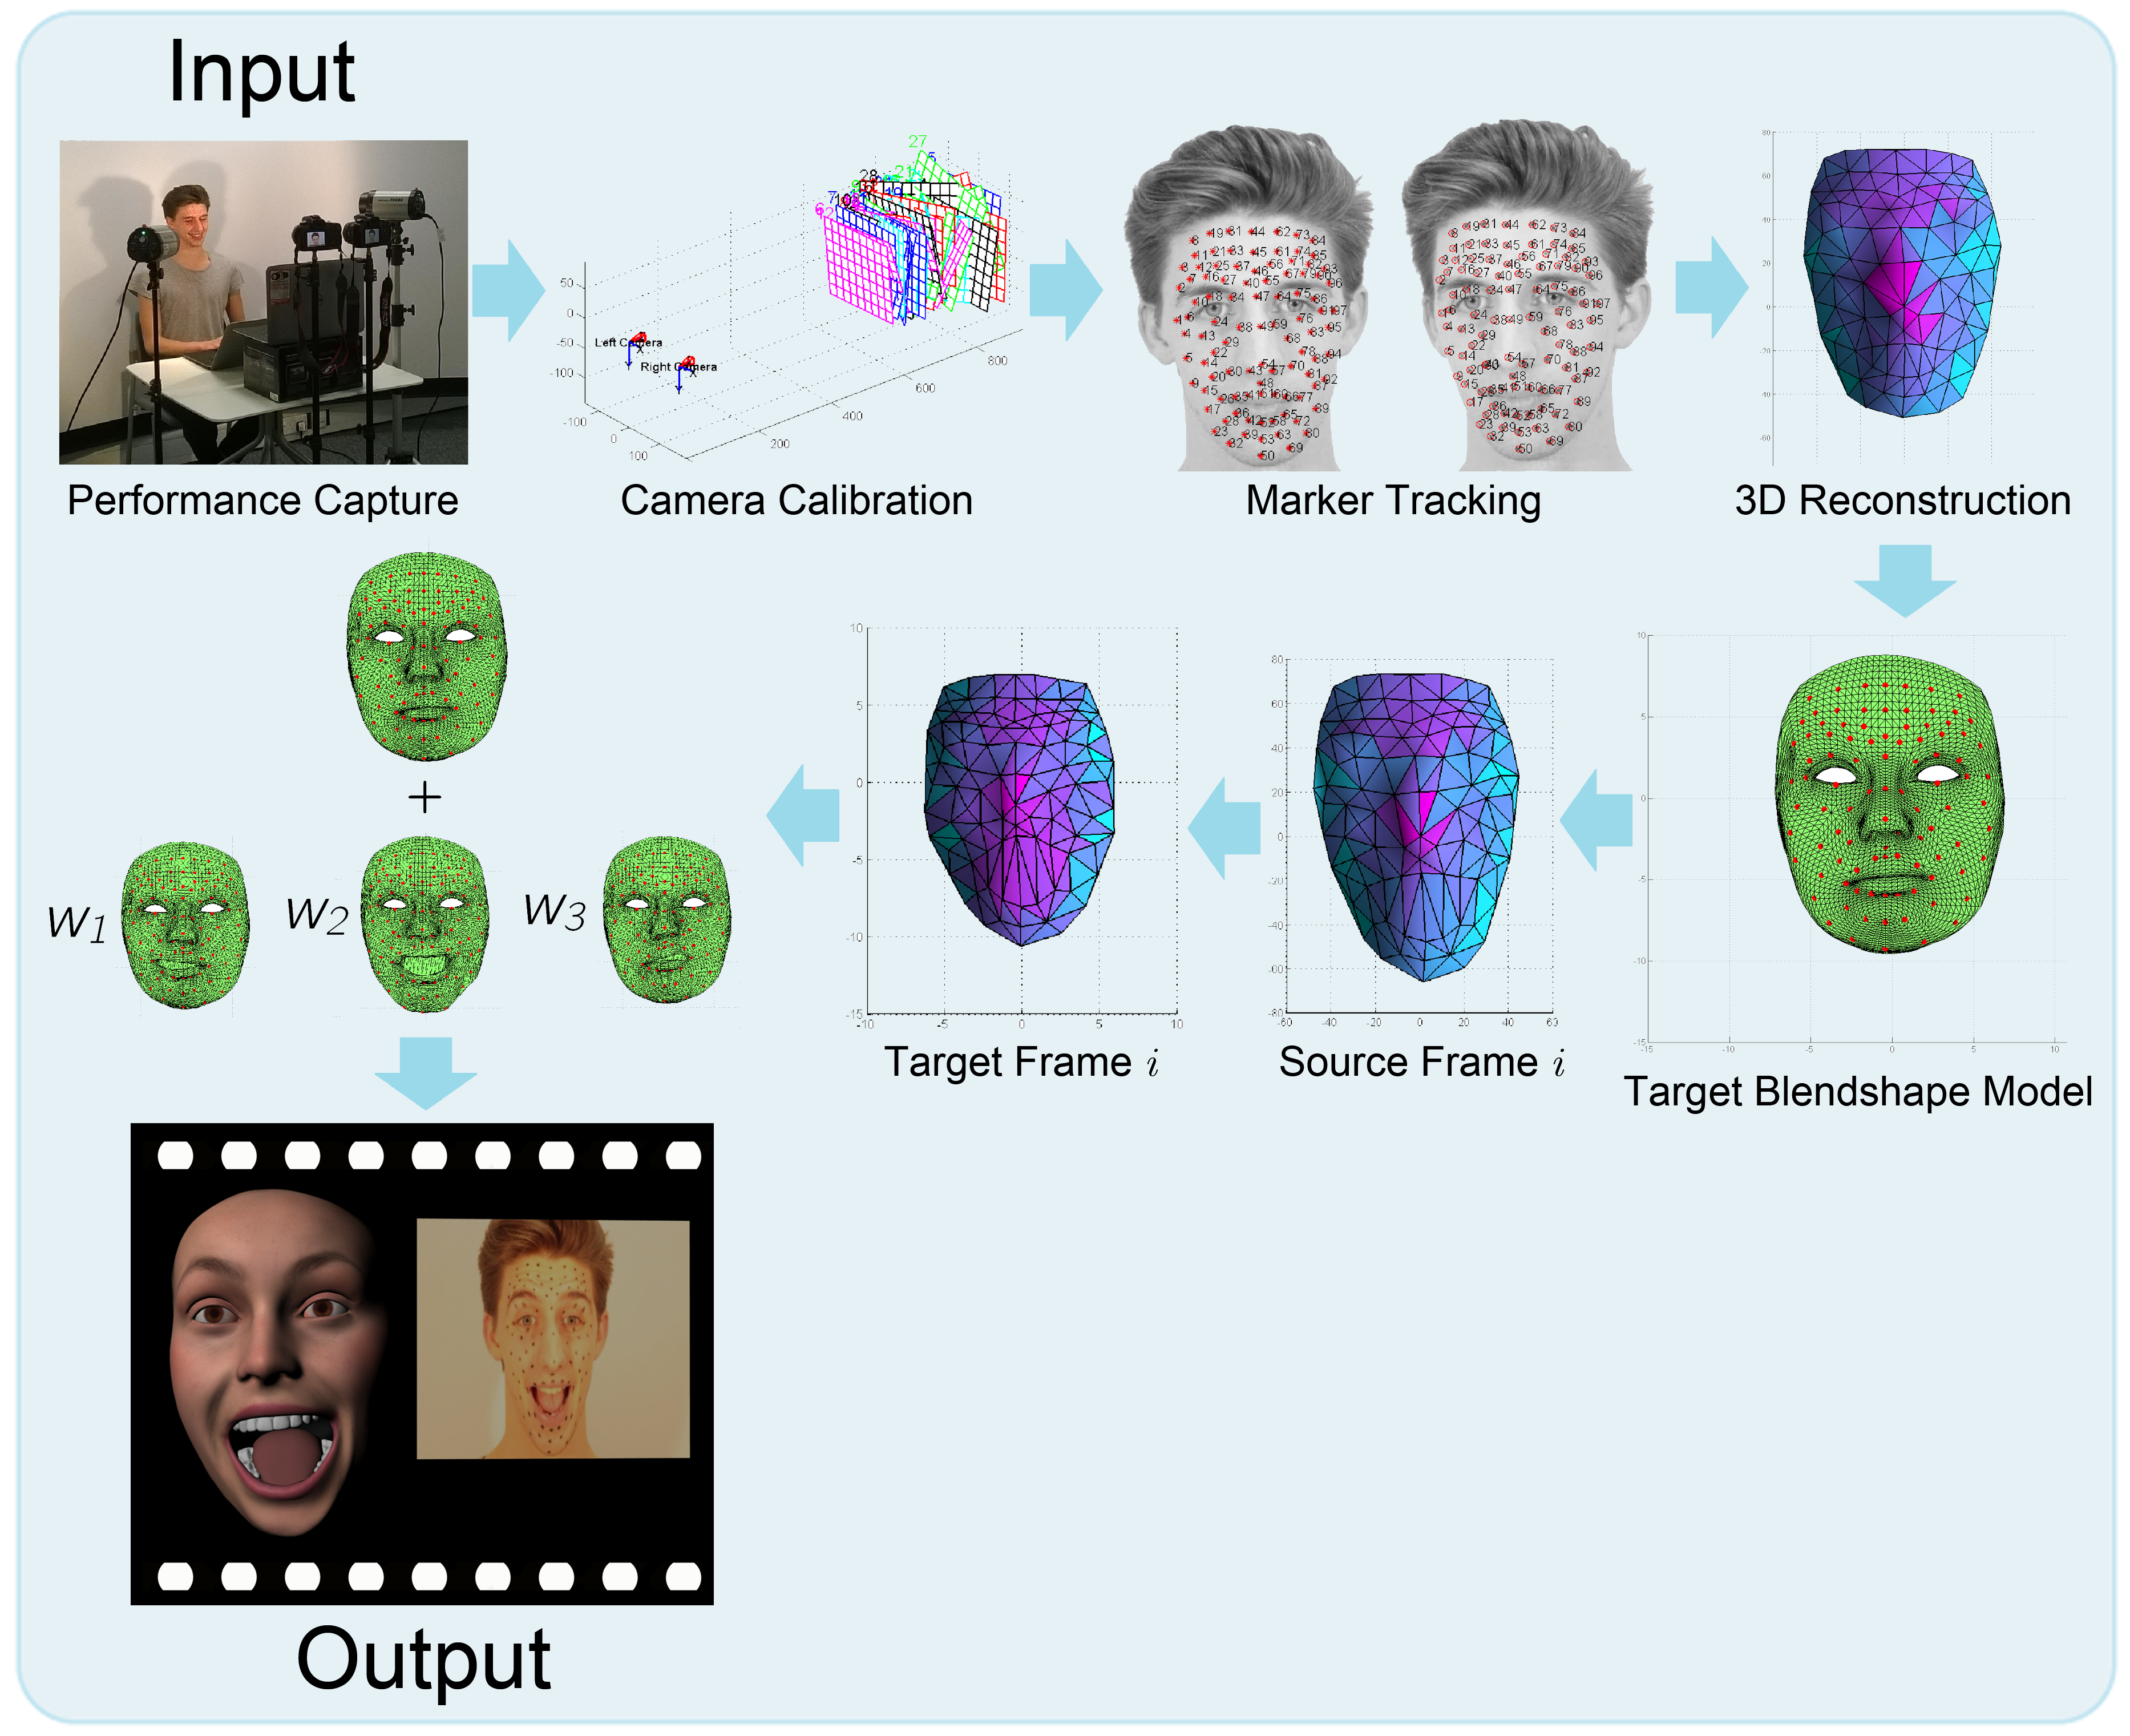
\includegraphics[width=\textwidth]{img/pipeline1}
	\caption{A schematic of the proposed pipeline for the performance capture system.}
	\label{fig:pipeline1}
\end{figure}

\section{Data Capture} \label{sec:datacapture}

The first task was to gather some initial input data for the system by recording the facial performance of an actor in the form of a video sequence. Two DSLR cameras were positioned close to the actor's face in a stereo configuration in order to capture the actor's facial performance, as shown in Figure \ref{fig:setup1}. A short sequence, consisting of the actor pulling a number of facial expressions and then talking, was recorded on video with a resolution of $640 \times 480$ at 60fps. The video streams were roughly synchronised afterwards during post-processing in the computer by aligning the two separate audio signals. A relatively low image resolution was chosen in order to try to limit the amount of video data we had to deal with, especially when recording sequences at higher frame-rates. The cameras were fixed on stands to prevent any camera-shake during the performance capture session and calibration process - since it is important that the camera positions remain static for accurate 3D reconstruction. Positioning the cameras close to one another, at approximately 10cm horizontal separation and at a distance of about 1m from the subject, meant that the images from both views would be quite similar - allowing for easier feature matching across the two images. However, the camera spacing was sufficiently large to enable both sides of the face to be in view, and to allow for triangulation of points on the actor's face; a good rule of thumb is for the cameras and subject to subtend an angle of at least 5 degrees.

\begin{figure}[htbp!]
\centering
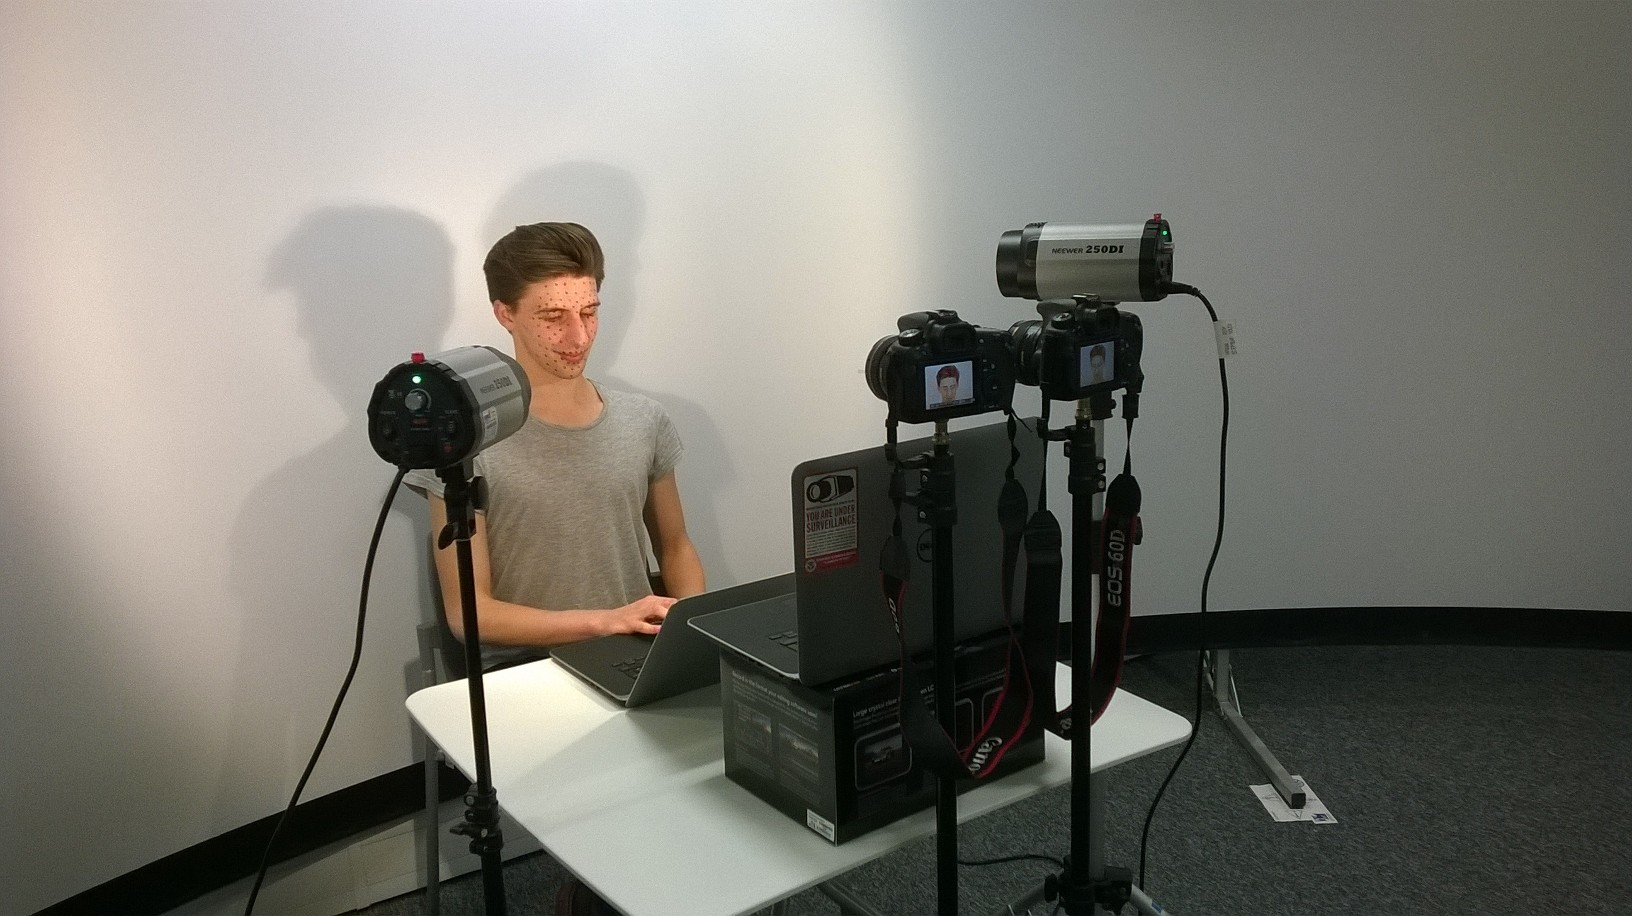
\includegraphics[width=\textwidth]{img/setup1}
	\caption{The stereo camera setup used to capture the facial performance.}
	\label{fig:setup1}
\end{figure}

Markers used to track the facial performance were placed on the actor's face in the configuration shown in Figure \ref{fig:facemarkers}. 97 markers were used in total, and were drawn onto the actor's face with a make-up pencil so as to be easily removed after the capture session. The positions of the markers were roughly based on those used in the Surrey Audio-Visual Expressed Emotion (SAVEE) Database ~\cite{Surrey}, as shown in Figure \ref{fig:surreydata}, although they use fewer markers with just 60 in total. In hindsight, using slightly fewer number of markers in our system might have been preferable, as consistently detecting and tracking a large number of markers (and preserving the labelling order of the markers) became quite a time-consuming and labour intensive process, prone to error. Furthermore, rather than simply using a black pencil, it might have advantageous to use markers of a significantly different colour to the tones of the human face in order to aid marker detection and tracking, or perhaps even using retro-reflective markers as in many commercial motion capture systems ~\cite{Vicon}.

Although the markers were placed all over the face to capture full facial performance, we tried to ensure that specific markers were placed in positions on the face which exhibit large non-rigid deformation, such as around the eyes, around the mouth and along the eye-brows, in order capture the full expressiveness of the face. In a future implementation, it would be useful to track the rigid head motion by tracking the positions of a number points on the head of the actor, for example by making the actor wear a skull cap with markers. Another useful addition would be to somehow track the eyelids so we can capture subtle eye movements and blinks. Also, since we only track points on the outside of the mouth, we do not gather information about the lip movement, such as expressions involving pursing or funnelling of the lips, etc.

\begin{figure}[htbp!]
\begin{minipage}[b]{0.47\textwidth}
\centering
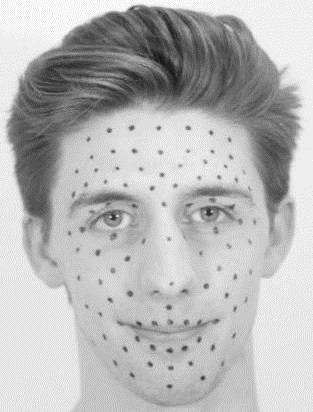
\includegraphics[width=\textwidth]{img/facemarkers}
	\caption{ The configuration of markers used for tracking the facial performance of the actor.}
	\label{fig:facemarkers}
\end{minipage}
\hfill
\begin{minipage}[b]{0.5\textwidth}
\centering
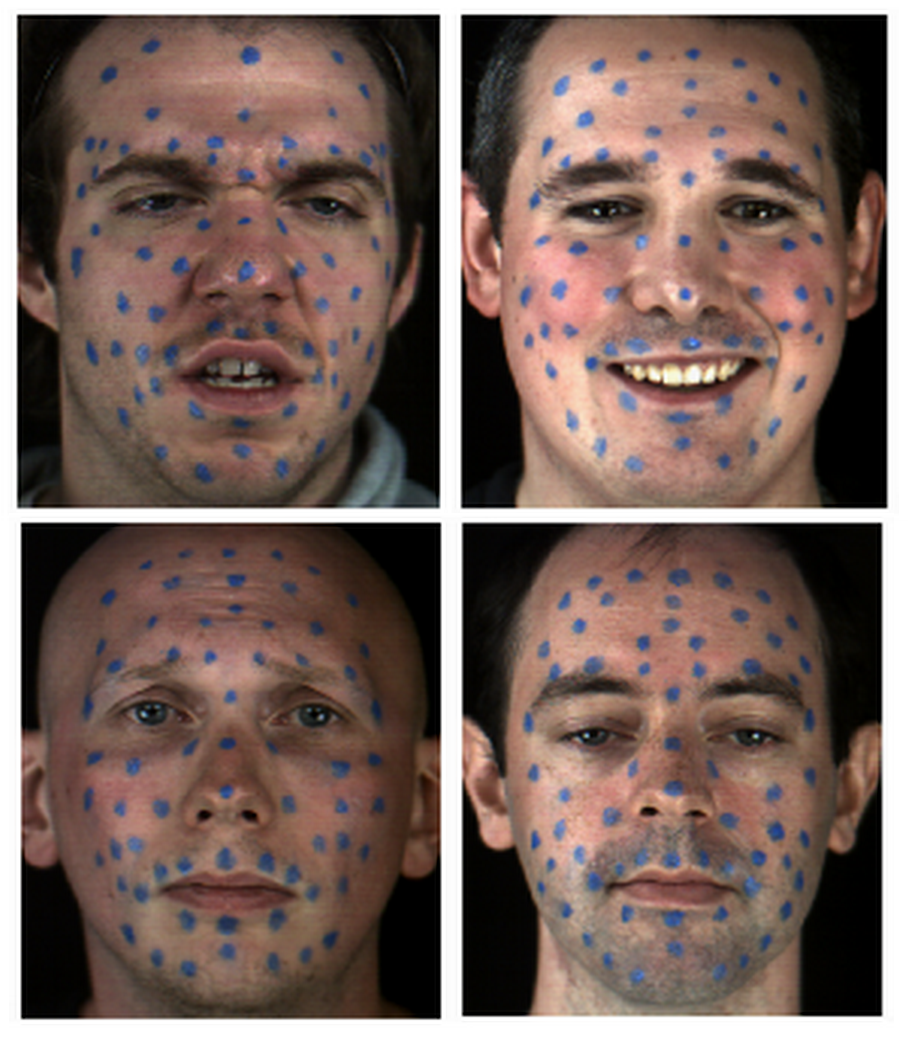
\includegraphics[width=\textwidth]{img/surreydata}
	\caption{ Images from the Surrey Audio-Visual Expressed Emotion (SAVEE) Database ~\cite{Surrey}.}
	\label{fig:surreydata}	
\end{minipage}
\end{figure}


\section{Camera Calibration}

Once we had obtained a video sequence of the actor's face, the next stage was to calibrate the stereo camera system in order to obtain accurate 3D coordinates of the markers on the face. 

Camera calibration is name given to the process of recovering the camera projection matrix $\vect{P}$ from images of a controlled scene. We assume the pinhole camera model and under perspective projection the map between the three-dimensional world coordinates of a point $(X, Y, Z)^T$ and its two-dimensional image pixel coordinates $(u, v)^T$ is a linear mapping in homogeneous coordinates represented by the $3 \times 4$ projection matrix:

\begin{equation}
\label{projection}
	\left(\!
    \begin{array}{c}
      su \\
      sv \\
      s
    \end{array}
  	\!\right) =
  \begin{bmatrix}
       p_{11} & p_{12} & p_{13} & p_{14} \\[0.3em]
       p_{21} & p_{22} & p_{23} & p_{24} \\[0.3em]
       p_{31} & p_{32} & p_{33} & p_{34}
  \end{bmatrix}
    \left(\!
    \begin{array}{c}
      X \\
      Y \\
      Z \\
      1
    \end{array}
    \!\right)
\end{equation}

To obtain an estimate of the camera projection matrices for both cameras, we use a checkerboard pattern of known dimensions held in a number of different positions and orientations throughout the scene, in view of both cameras simultaneously, as shown in Figure \ref{fig:checkerboard}. To perform the calibration, we made use of the Camera Calibration Toolbox for Matlab \cite{Calib} provided by Jean-Yves Bouguet, which automatically detects the grid corners in each image and solves for the intrinsic camera parameters (focal length, principle point, and distortion coefficients) and the extrinsic parameters (rigid rotation and translation). It was important to ensure that the checkboard remained within the frame of both cameras during the entire calibration process, and that the camera positions did not move between the performance capture session and the calibration procedure. 

\begin{figure}[htbp!]
\centering
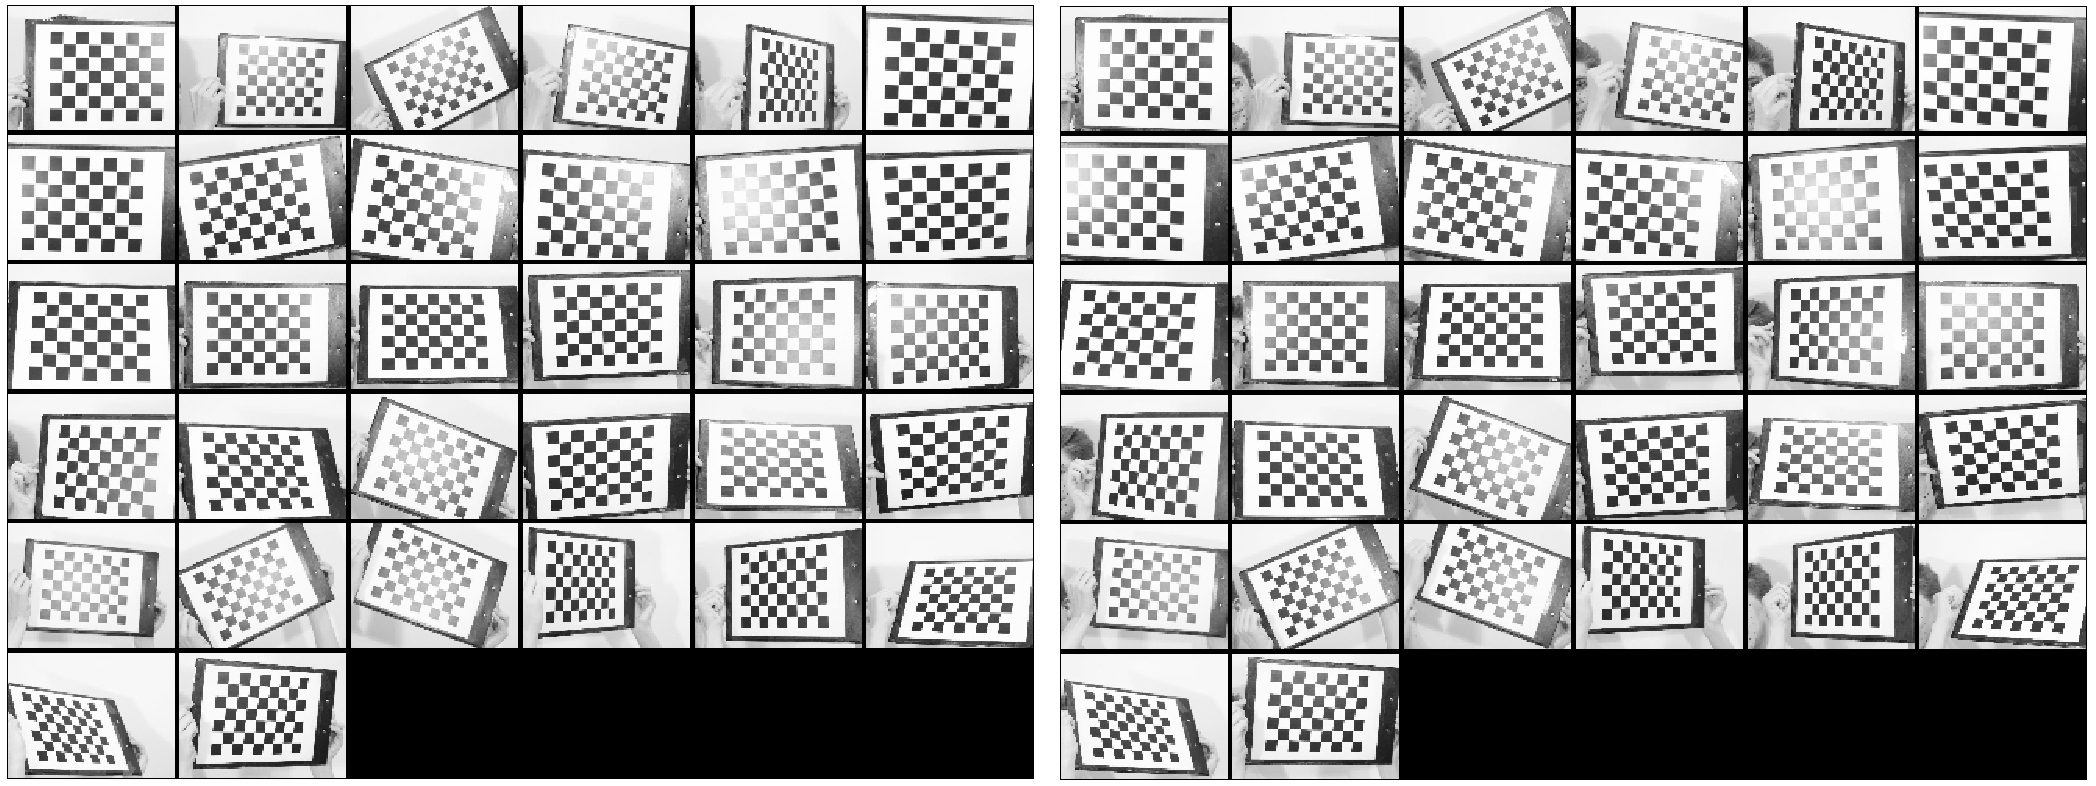
\includegraphics[width=0.9\textwidth]{img/calib2}
	\caption{A checkerboard pattern was used to calibrate the pair of stereo cameras. The checkerboard had to be visible from both camera viewpoints simultaneously.}
	\label{fig:checkerboard}
\end{figure}

As a result of the stereo calibration, we obtain an estimate of the intrinsic matrices $\vect{K}$, $\vect{K}'$ and external parameters $\vect{R}$, $\vect{t}$ of the two cameras, from which we can compute the camera projection matrices $\vect{P}$ and $\vect{P}'$ for the left and right cameras respectively using the equation for perspective projection:

\begin{equation*}
\label{qrdecomp}
	\left(\!
    \begin{array}{c}
      su \\
      sv \\
      s
    \end{array}
  	\!\right) =
  \vect{K}[\vect{R}|\vect{t}]
    \left(\!
    \begin{array}{c}
      X \\
      Y \\
      Z \\
      1
    \end{array}
    \!\right) 		 
\end{equation*}

\begin{equation*}
\left(\!
    \begin{array}{c}
      su \\
      sv \\
      s
    \end{array}
  	\!\right) =
  \begin{bmatrix}
       fk_u & 0 & u_0 \\[0.3em]
       0 & fk_v & v_0 \\[0.3em]
       0 & 0 & 1
  \end{bmatrix}
    \begin{bmatrix}
       r_{11} & r_{12} & r_{13} & t_x \\[0.3em]
       r_{21} & r_{22} & r_{23} & t_y \\[0.3em]
       r_{31} & r_{32} & r_{33} & t_z
  \end{bmatrix}
    \left(\!
    \begin{array}{c}
      X \\
      Y \\
      Z \\
      1
    \end{array}
    \!\right)
\end{equation*}

where the left camera is assumed to be centred at the origin and aligned with the world co-ordinate axes, i.e. its projection matrix is $\vect{P} = \vect{K} [\vect{I} | \vect{0}]$, and the right camera projection matrix is expressed as $\vect{P}' = \vect{K}' [\vect{R} | \vect{t}]$.

The resulting extrinsic parameters, describing the rotation $\vect{R}$ and translation $\vect{t}$ between the two camera views, are visualised in Figure \ref{fig:calib}. The positions of the checkerboard used for calibration are also displayed.

\begin{figure}[htbp!]
\centering
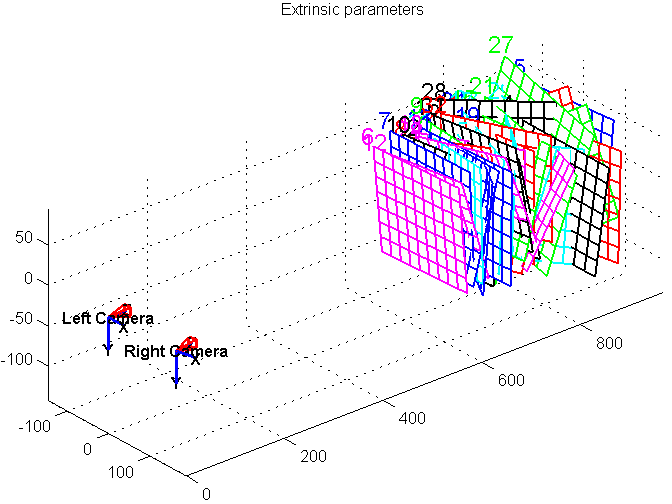
\includegraphics[width=0.8\textwidth]{img/calib}
	\caption{The resulting extrinsic parameters of the calibrated stereo camera setup.}
	\label{fig:calib}
\end{figure}

From the estimated projection matrices, we can compute an estimate of the fundamental matrix $\vect{F}$ relating the two camera views. The fundamental matrix encapsulates the intrinsic epipolar geometry algebraically and is defined by the following equation:

\begin{equation*}
\vect{u'}^T \vect{Fu} = 0
\end{equation*}

\begin{equation*}
(u' v' 1)
    \begin{bmatrix}
    f_{11} & f_{12} & f_{13} \\
    f_{21} & f_{22} & f_{23} \\
    f_{31} & f_{32} & f_{33}
    \end{bmatrix}
    \left(\!
    \begin{array}{c}
     u \\
  	 v \\
   	 1  
    \end{array}
    \!\right) = 0
\end{equation*}

where $\vect{u} = (u,v,1)^T$ and $\vect{u}'= (u',v',1)^T$ are the 2D pixel coordinates of the same 3D world point imaged in the left and right views respectively. The fundamental matrix $\vect{F}$ is a $3 \times 3$ matrix, so has 9 elements but only has 7 DoF. This is because it has arbitrary scale, leaving 8 DoF, and is of rank 2 and singular, i.e. $\mathrm{det} [\vect{F}] = 0$, leaving 7 DoF. Using the fundamental matrix relation, the equation of the epipolar line in the right image $\vect{l}'$ corresponding to the point $\vect{u}$ in the left image, on which the feature point must lie, is therefore given by the following expression

\begin{equation}
\vect{l}' = \vect{Fu}
\end{equation} 

Similarly, the epipolar line $\vect{l}$ in the left image is given by

\begin{equation*}
\vect{l} = \vect{F}^T \vect{u}'
\end{equation*} 

The left and right epipoles $\vect{e}$ and $\vect{e}'$ are defined as the point in each image which is common to all the epipolar lines and are given by the null spaces of $\vect{F}$ and $\vect{F}^T$ respectively

\begin{equation*}
\vect{Fe} = \vect{0} \ \ \ \ \ \ \
\vect{F}^T\vect{e}' = \vect{0}
\end{equation*} 

With the epipolar geometry fully defined, we can then rectify the stereo images for every frame of the captured image sequence so that the eipolar lines are horizontal. This reduces the stereo matching problem to a 1D search problem, as the same 3D world point imaged in both cameras is constrained to lie on the same pixel row in each pair of images. To rectify each pair of stereo images we implemented a function in Matlab \texttt{StereoRectify.m}, based on the function \texttt{rectify\_stereo\_pair.m} provided in the Camera Calibration Toolbox for Matlab \cite{Calib} which rectifies each pair of calibration images. This works as follows: we first bring the two cameras into the same orientation by rotating them 'minimally', so as to bring the translation vector $\vect{t}$ in alignment with the positive $x$-axis $(1,0,0)^T$. Global rotations are applied to both cameras so that the resulting rigid motion between the cameras is just a translation and the rotation matrix becomes $\vect{R} = \vect{I}$. The vertical component of the estimated focal length $f_u$ must be the same in both images and we set the horizontal focal length $f_v$ to the same as the vertical, resulting in square pixels, and new principle points are chosen to be the average of the two principle points. New camera projection matrices are computed accordingly and we warp each image so that the epipolar lines are horizontal. A pair of rectified images for a frame of the captured image sequence is shown in Figure \ref{fig:epipolarlines}. Matching image points and their corresponding epipolar lines are plotted.

\begin{figure}[htbp!]
\centering
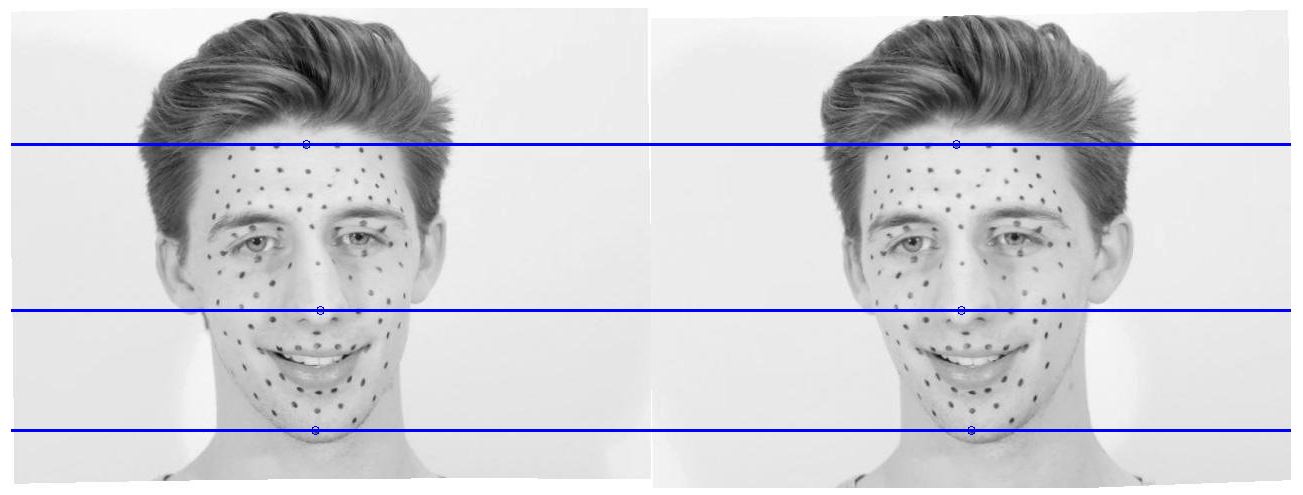
\includegraphics[width=\textwidth]{img/epipolarlines}
	\caption{Using the stereo calibration results, each pair of images in a captured image sequence is rectified so that corresponding epipolar lines lie on the same pixel row. This reduces the stereo correspondence problem to a 1D search along the epipolar lines.}
	\label{fig:epipolarlines}
\end{figure}

\section{Initial Marker Detection}

The facial markers are detected in the first frame of a captured image sequence and then are tracked throughout the length of the sequence. The initial marker detection is achieved by detecting SIFT features in the image. We employ the open source Matlab implementation VLFeat \cite{vedaldi08vlfeat} to do this. 

The marker detection process for the first frame of a given stereo image sequence is carried out as follows. First the user defines a region of interest in the left image around the face of the actor to be tracked, by drawing a contour in the image. We make use of the Matlab function \texttt{roipoly} for this. Then, SIFT features are detected within the selected image region, choosing the appropriate SIFT parameters to pick out features of around 5 pixels in diameter - this may take a few tries to get right. Once reasonable SIFT features have been detected, additional feature points can then be added manually, and also wrongly detected points can be removed, by interactively selecting certain points the user wishes to change. Once the user has successfully detected all 97 facial markers in the left image, the corresponding marker positions are found in the right image by searching along the corresponding epipolar lines; simply the same row of pixels in the right image since the images have been stereo rectified beforehand. The matching points in the right image are found by computing the normalised cross-correlation between image patches:

\begin{equation}
\begin{aligned}
	C_{NCC} = \sum_{i=1}^N \frac{(I_i^L - \mu^L)(I_i^R - \mu^R)}{\sigma^L \sigma^R}
\end{aligned}
\end{equation}

\begin{figure}[htbp!]
\centering
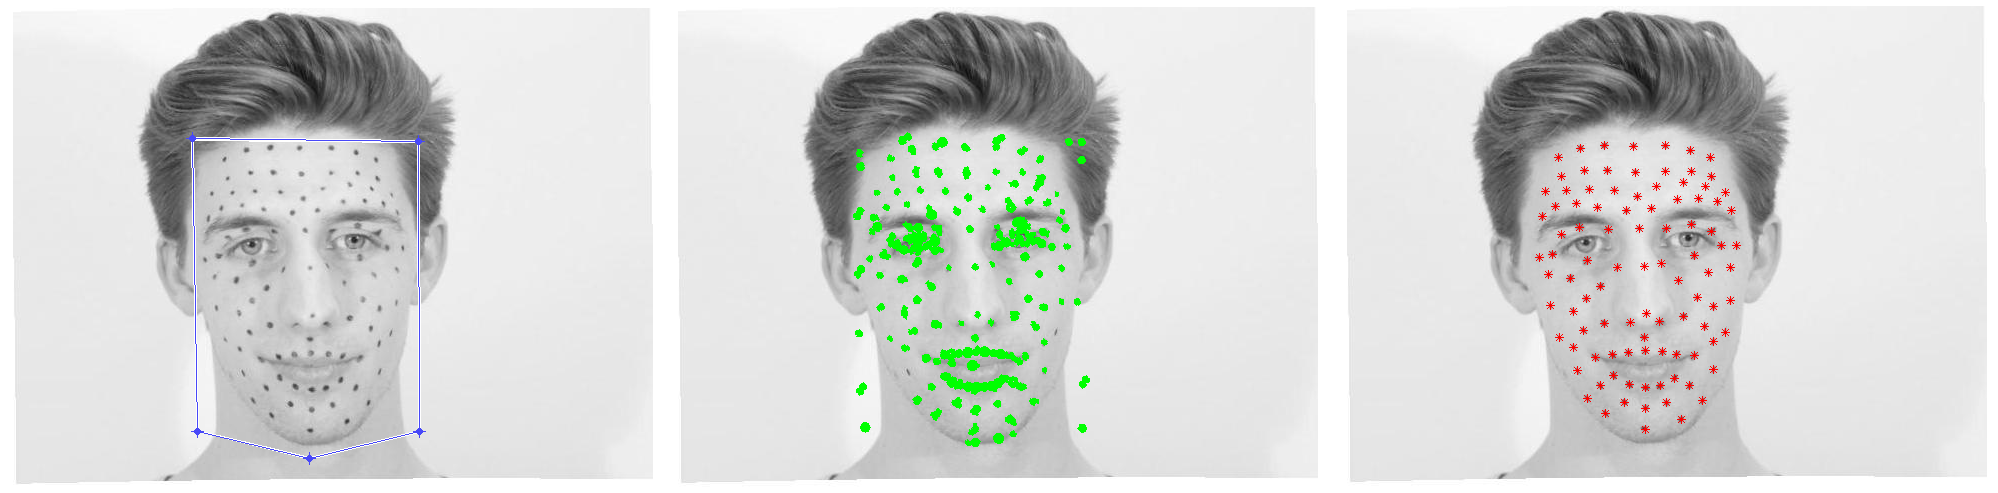
\includegraphics[width=\textwidth]{img/detection}
	\caption{Facial markers are detected by first selecting a region of interest, detecting SIFT features, and then removing unwanted points or adding additional points.}
	\label{fig:detection}
\end{figure}

\begin{figure}[htbp!]
\centering
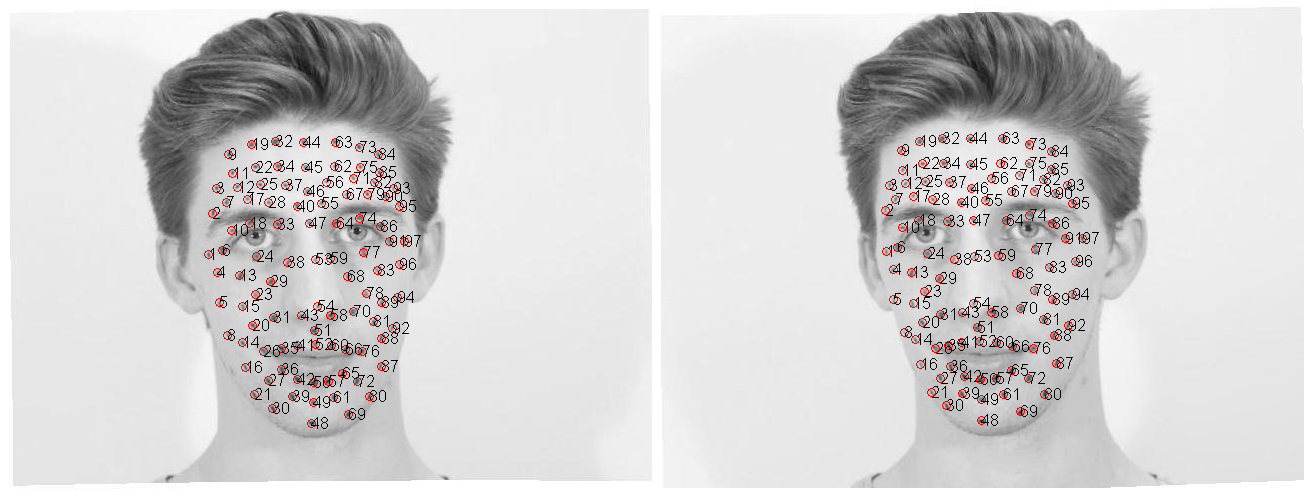
\includegraphics[width=\textwidth]{img/matching}
	\caption{Detected facial markers in the left image are matched to markers in the right image pair by computing the normalised cross-correlation between image patches around the points.}
	\label{fig:matching}
\end{figure}

\section{Marker Tracking}

With the facial markers detected in the first frame, the next task was to track the positions of the markers as they move throughout the image sequence. 

\subsection{Optical Flow}

\subsection{KLT Tracker}

\cite{Shi:1994}

\subsection{Kalman Filter}

\section{Sparse Facial Reconstruction}

Once we have obtained the 2D image coordinates of the facial markers for every frame in a stereo image sequence, we then compute the sparse 3D reconstruction over the sequence. In one frame, given a pair of image correspondences $\vect{w} = (u,v,1)^T$ and $\vect{w}' = (u',v',1)^T$ of the same 3D point $\vect{X} = (X,Y,Z,1)^T$, we can write two equations using the projection matrices $\vect{P}$ and $\vect{P'}$:

\begin{equation}
\left(\!
    \begin{array}{c}
      su \\
      sv \\
      s
    \end{array}
  	\!\right) = \vect{P}
  	\left(\!
    \begin{array}{c}
      X \\
      Y \\
      Z \\
      1
    \end{array}
  	\!\right) 
  	\ \ \ \ \ \ \ \ 
\left(\!
    \begin{array}{c}
      su' \\
      sv' \\
      s
    \end{array}
  	\!\right) = \vect{P'}
  	\left(\!
    \begin{array}{c}
      X \\
      Y \\
      Z \\
      1
    \end{array}
  	\!\right).
\end{equation}
For each pair of image points, two equations can be written:

\begin{align*}
u &= \frac{p_{11}X + p_{12}Y + p_{13}Z + p_{14}}{p_{31}X + p_{32}Y + p_{33}Z + p_{34}} \ \  
u' = \frac{p'_{11}X + p'_{12}Y + p'_{13}Z + p'_{14}}{p'_{31}X + p'_{32}Y + p'_{33}Z + p'_{34}}\\ 
v &= \frac{p_{21}X + p_{22}Y + p_{23}Z + p_{24}}{p_{31}X + p_{32}Y + p_{33}Z + p_{34}} \ \ 
v' = \frac{p'_{21}X + p'_{22}Y + p'_{23}Z + p'_{24}}{p'_{31}X + p'_{32}Y + p'_{33}Z + p'_{34}}
\end{align*}
Rearranging, these can be written in the form $\vect{AX} = 0$ as follows, where $\vect{p}_i$ denotes the $ith$ row of the projection matrix $\vect{P}$

\begin{equation}
\begin{bmatrix}
       u\vect{p}_3^T - \vect{p}_1 \\[0.3em]
       v\vect{p}_3^T - \vect{p}_2 \\[0.3em]
       u' \vect{p'}_3^T - \vect{p'}_1 \\[0.3em]
       v' \vect{p'}_3^T - \vect{p'}_2
\end{bmatrix}
\left(\!
    \begin{array}{c}
      X \\
      Y \\
      Z \\
      1
    \end{array}
  	\!\right) = 0.
\end{equation}
Two equations are acquired from each image point in the two views, giving a total of four equations with three unknowns - the problem is over-constrained. A linear least-squares solution can be found by performing Singular Value Decomposition on the matrix $\vect{A}$. The 3D coordinates of the point $\vect{X}$ are the singular vector corresponding to the smallest singular value of $\vect{A}$, i.e. the last column of the matrix $\vect{V}$, where $\vect{A} = \vect{UDV}^T$. This is implemented in Matlab in the function \texttt{Reconstruct.m}, which takes in the two camera projection matrices for a pair of stereo cameras and the matching 2D image points, and returns an array of corresponding 3D points.

\begin{figure}[htbp!]
\centering
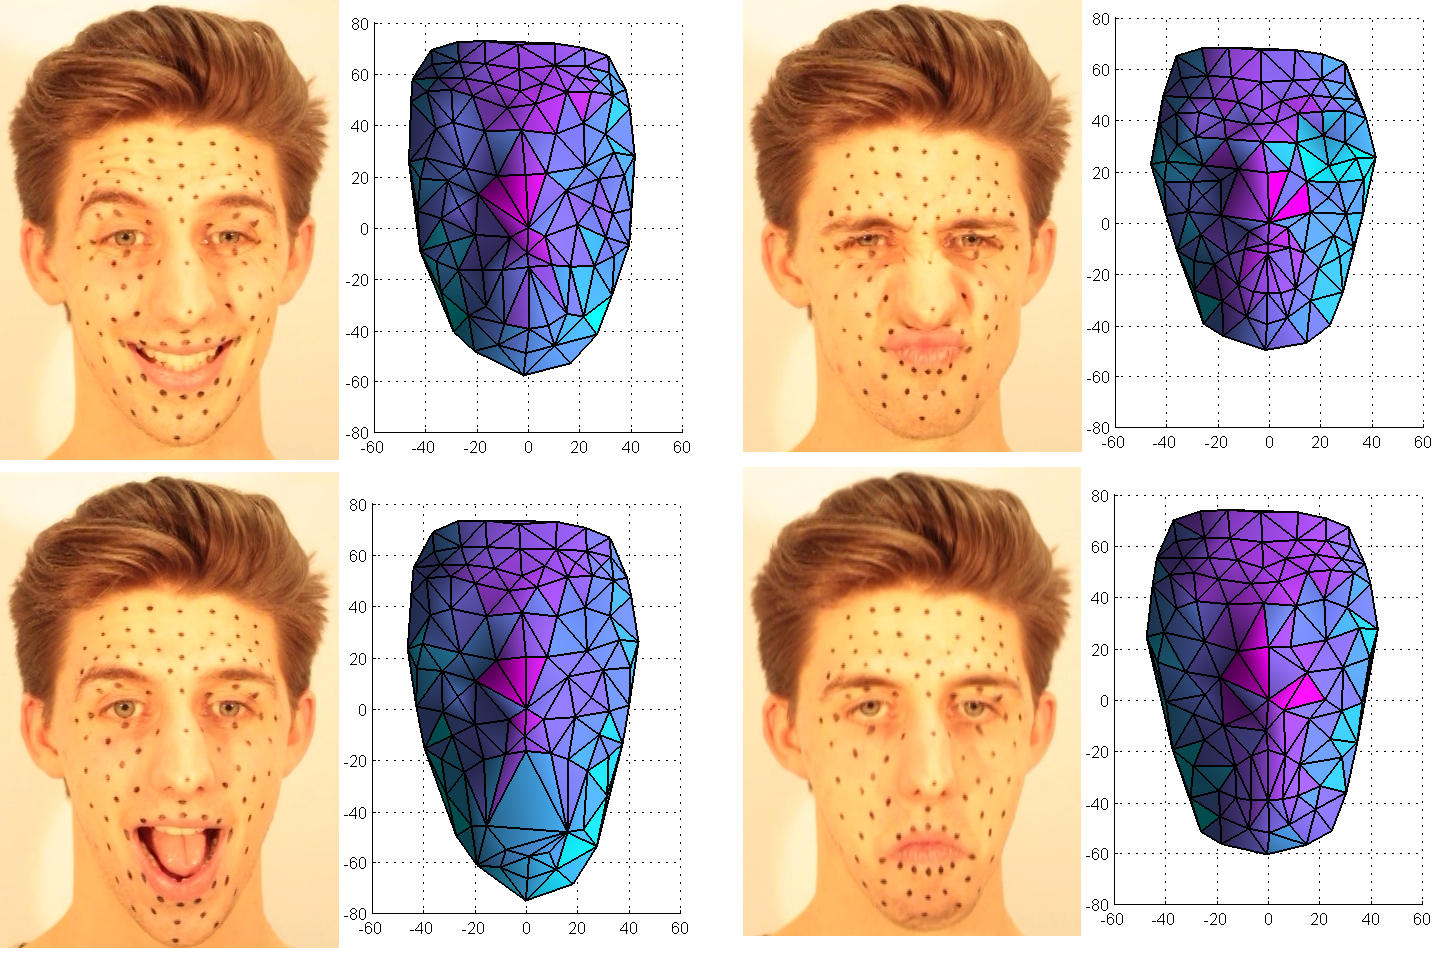
\includegraphics[width=\textwidth]{img/faces}
	\caption{A sparse 3D reconstruction is computed for every frame of an image sequence using the detected marker positions and the calibrated camera projection matrices. A sample of image frames and the corresponding 3D reconstructions are shown above.}
	\label{fig:faces}
\end{figure}

\subsection{Stabilising Head Movement}
\label{sec:stabilising_head_movement}

It is important for the actor's head to remain still throughout the sequence so that the reconstructed facial expressions are expressed as true non-rigid deviations from the neutral facial expression. Proper stabilisation of the head is required to avoid artefacts in the resulting blendshape facial animation and retargeting process \cite{Beeler:2014}. If the rigid head movement is not removed, then the expression shapes will contain this 'baked-in' rigid motion, and any facial animation constructed from the expressions will also contain this unwanted rigid head motion. In industry, face-stabilisation is still usually performed manually; Weise \textit{et al}. \cite{Weise:2009} aim to remove the rigid motion component of multiple expressions using ICP registration and Vlasic \textit{et al}. \cite{Vlasic:2005} use Procrustes alignment.

In our implementation, we attempt to remove the majority of the actor's rigid head motion by performing a Procrustes analysis \cite{Gower:1975} using a number of approximately rigid points. At least four points are required for the Procrustes alignment. The rigid points were chosen to be the tops of the ears, the tip and bridge of the nose, and the centre point on the top of the forehead, as shown by the dots in Figure \ref{fig:procrustes}. However, none of these points are actually truly rigid, so this is just an approximation to the true stabilisation. In a future implementation, it would be better to actually track a few points known to be practically rigid, for example by placing markers on the top of the head. 

The Procrustes analysis computes a least-squares fit of each facial expression in a given frame to the neutral face, given the rigid vertex correspondences. In Figure \ref{fig:procrustes}, the rigid correspondences are plotted in red for the neutral face, and blue for a particular frame. We do this for the entire image sequence so that in every frame the head pose is aligned to the neutral position. We have found that the average error over an image sequence is usually around the order of $10^{-3}$. However, it is not simply the case that the smaller the error means the better the alignment of the expression to the neutral face, because the head can be orientated in such a way that can make the error in the rigid vertex correspondences small, but can result in an unnatural head pose. Through experimentation, we have found that choosing points that span the entire face and are placed the extremities of the face, such as the ears, generally results in a better alignment than rather selecting a few points close together around the centre of the face, such as around the mostly rigid nose region. This makes sense because a small deviation in points around the centre of mass will lead to larger displacements in the other points, whereas small deviations in points at the edges will have much less of an impact on points in the centre of the face. 

\begin{figure}[htbp!]
\centering
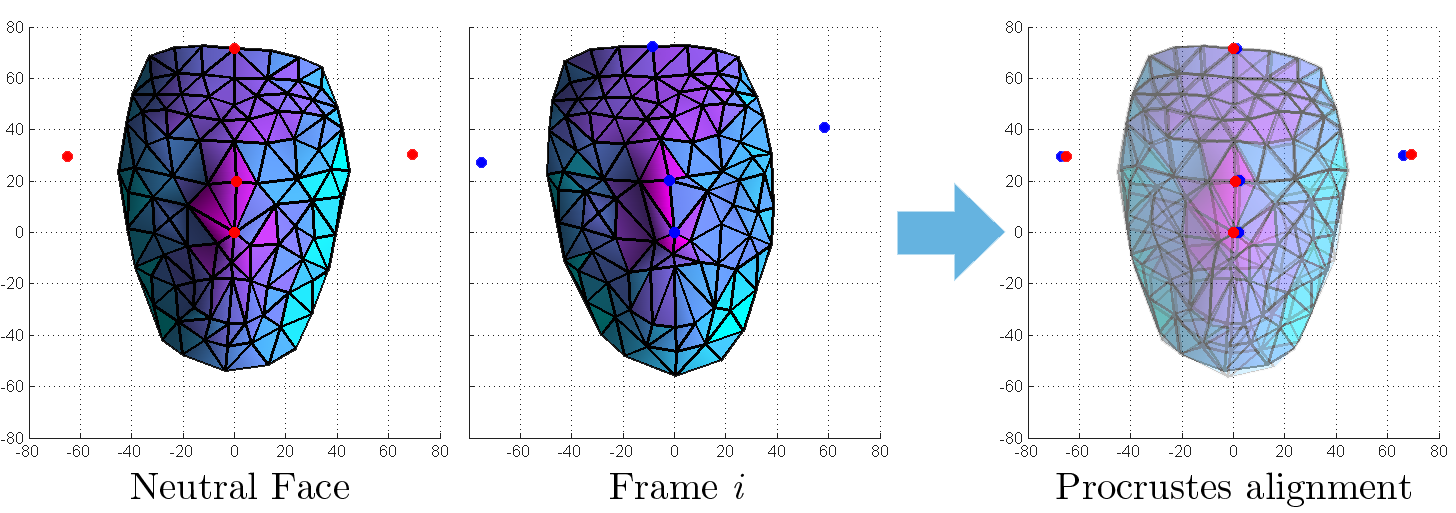
\includegraphics[width=\textwidth]{img/procrustes}
	\caption{The head pose in each frame of an image sequence is aligned to the neutral face position using Procrustes analysis. The rigid vertex correspondences are shown in red for the neutral pose, and blue for a given frame.}
	\label{fig:procrustes}
\end{figure}

\section{Facial Animation}
Given the motion capture data, our goal is to produce an animation that resembles the captured motion. We use the Digital Emily model designed by Alexander et al.~\cite{Alexander:2009}. In this section we introduce the techniques used to match three-dimensional surfaces and point clouds, and the optimisation methods used to estimate the parameters that describe the motion of the digital model.

\subsection{Thin Plate Splines}\label{sec:tps}
Thin plate theory addresses problems that commonly arise in areas of natural sciences and engineering when trying to model the behaviour of a thin sheet of some material. The possible processes include but are not limited to stretching, bending, crumpling, buckling, shrinking, straining and tearing. The corresponding mathematical model is based on ideas from differential geometry as well as continuum mechanics, and the set of equations describing the aforementioned phenomena are often notoriously difficult to solve. Therefore, in Computer Graphics, as well as other fields, a number of simplifying assumptions are made when constructing a thin plate model. 

A thin plate is considered to be a two dimensional object, i.e. it is assumed that the thickness is infinitesimal. The geometry of the object is often simplified to reduce the computational cost. Thin plate splines (TPS) are a two-dimensional counterpart of the cubic spline~\cite{Sibson:1991}. TPS are a deformation method based on the assumption that a thin surface deforms in a way that minimises the surface bending energy. The bending energy is proportional to the change in the second fundamental form. Specifically, given two corresponding sets of point $\{(x_i, y_i\}_i^N$ and $\{v_i\}_i^N$ there exists a height field mapping between the two, $f: \mathbb{R}^2 \to \mathbb{R}$. The bending energy corresponding to this mapping is proportional to the second order derivatives of the mapping:
\begin{equation}
\begin{aligned}
	E_{bend}(f) = \lambda \iint \left( \left( \dfrac{\delta^2f}{\delta x^2} \right)^2 +  2 \left( \dfrac{\delta^2f}{\delta x y} \right)^2 +  \left( \dfrac{\delta^2f}{\delta y^2} \right)^2 \right) \dd x \dd y,
\end{aligned}
\end{equation} where $\lambda$ is smoothing parameter, which balances the quality of fit and the amount of bending, i.e. the wiggliness of the function. TPS finds the transformation that fits the data while minimising the bending energy. Note that TPS may also be defined in terms of the radial basis functions that are used for smooth scattered data fitting. The RBF solution for thin plate splines is:
\begin{equation}
\begin{aligned}
	f(x,y) = \sum_{i=1}^N \omega_i \: \phi(\|(x,y) - (x_i,y_i)\|), \: \text{ where} \: \phi(r) = r^2 \log(r).
\end{aligned}
\end{equation} To ensure that the function $f$ has square-integrable second derivatives, the following conditions are imposed:
\begin{equation}
	\sum_{i=1}^N \omega_i = \sum_{i=1}^N \omega_i x_i = \sum_{i=1}^N \omega_i y_i = 0.\label{eq:TPSrestrictions}
\end{equation} These conditions and the data fitting requirement may be combined into a linear system of equations:
\begin{equation}
\begin{bmatrix}
	K & P \\
	P^T & 0 
\end{bmatrix} 
\begin{bmatrix}
	\omega \\
	o
\end{bmatrix} = 
\begin{bmatrix}
	v \\
	o
\end{bmatrix}, 
\end{equation} where $K$ encodes the relation between the data points, i.e. $K_{ij} = \phi(\|(x_i,y_i) - (x_j,y_j)\|)$, $P_{i\cdot} = (1, x_i, y_i)$ contains the variables from Eq.~\ref{eq:TPSrestrictions}, $\omega$ contains the values of $\omega_i$, and $v$ contains the target function values $v_i$. The variables $0$ and $o$ denote the zero matrix and the zero column vector respectively. Solving this linear system of equations gives the desired transformation in two dimensions. The method extends naturally to three-dimensional problems by including a dependence on an additional variable in the calculations described above. Radial basis functions are commonly used in the field of performance-driven animation~\cite{Joshi:2003}.

\subsection{Non-Rigid ICP}
Iterative Closest Point (ICP) is an algorithm used to align two partially overlapping point clouds by minimising the square error between corresponding points. The quality of the results produced by this algorithm is sensitive to the initial guess at a solution, i.e. ICP only refines the initial estimation. See Alg.~\ref{alg:icp} for the outline of the algorithm. Mean square error algorithm is used to calculate the average of the squared errors between the target and the transformed source points. Thus the objective function is a function of rotations and translations. The output of the algorithm is a transformation matrix that provides the optimal mapping between the two point clouds within a given threshold. The transformation matrix may be split into rotation and translation. The algorithm solves a linear system of equations where the unknowns are the coefficients in the rotation matrix and the translation vector and the known point cloud values are used as coefficients. The method is often used to find a transformation between a point cloud and a surface; in that case the surface normals are used as additional input.

\begin{algorithm}[H]   \caption{Iterative Closest Point.}
\KwData{source point cloud \\
\hspace{0.9cm} target point cloud\;
\hspace{0.9cm} initial guess\;
\hspace{0.9cm} error threshold\;
 }
\BlankLine
\While{error $>$ threshold}{
\For{point in source}{
  find closest point in target\;
  }
use mean squared error to find best transformation that aligns source to target \;
apply transformations\;
}
 \label{alg:icp}
\end{algorithm} 
The original ICP algorithm is limited to rigid transformations, i.e. rotation and translation, which have only $6$ degrees of freedom. However, in order to capture scaling, shearing and other more complicated transformation, an affine mapping should be used. Thus an extension of the ICP algorithm, called non-rigid ICP is used when additional degrees of freedom are present. Allen et al. proposed a non-rigid registration method that uses a numerically non-linear solver to find a smooth affine mapping~\cite{Allen:2003}. Additional constrained are imposed by manually matching some known marker locations in the two datasets. The method exhibits slow convergence and often leads to local minima; consequently, the authors use a multi-resolution approach where the optimisation is first performed on a low resolution mesh, and then optimised on the high resolution mesh. Amberg et al. combined the ICP algorithm with the method of Allen et al. to overcome the issues with convergence~\cite{Amberg:2007}.

\subsection{Animation}
The aim of this project is to used captured data of a face to animate a given model. We use the digital Emily model that comes with $68$ controllable blendshapes ranging from simple eyebrow movements to complicated lip corner pulls~\cite{Alexander:2009},~\cite{FaceWareRigsWeb}. Each blendshape has a weight $w_i$ associated with it, and $w_i \in [0,1]$. The model includes eyes and teeth. The aim is to find a combination of these blendshapes that produce a specified facial expression. In particular, we are interested in reproducing the captured sequence of expressions. 

\subsubsection{Initial Approach}
We manually choose a sparse set of points that corresponds to the sparse source mesh. Then the neutral expression of the subject is matched with the neutral expression of Emily by transforming the sparse source mesh to the sparse target mesh using TPS. The transformation is stored, and it is used to map all the frames in the captured sequence. This produces a sparse Emily sequence; using TPS again we warp the dense Emily mesh according to the positions of the sparse points. The quality of the resulting animation is poor for a number of reasons. Firstly, the sparse points are not able to constrain the dense mesh, especially since parts of the face, for example the eyelids and the lips are not tracked in the sparse mesh. Consequently, numerous artefacts appear on the dense mesh, and they are particularly noticeable around the lips as no boundary conditions are imposed. Secondly, though there is a clear correspondence between the generated Emily sequence and the source sequence, the generated expressions look unnatural. This may be explained by the differences in the geometry and anatomy of the two faces; for instance, the source may be able to pull expressions that cannot be mimicked by the model. In addition, the errors in tracking, reconstruction, and manual selection of sparse points on Emily further reduce the quality of the animation.

Our initial attempt to improve the method involved simplifying the dense Emily model by removing the part of the mesh that corresponds to the lips. Though the simpler mesh exhibited slightly better behaviour, i.e. there were fewer visible artefacts, the sparse point cloud was still unable to constrain the dense mesh well enough to produce realistic results, see Fig.~\ref{fig:ghost}. 
\begin{figure}[htbp!]
        \centering
        \begin{subfigure}[b]{0.45\textwidth}
                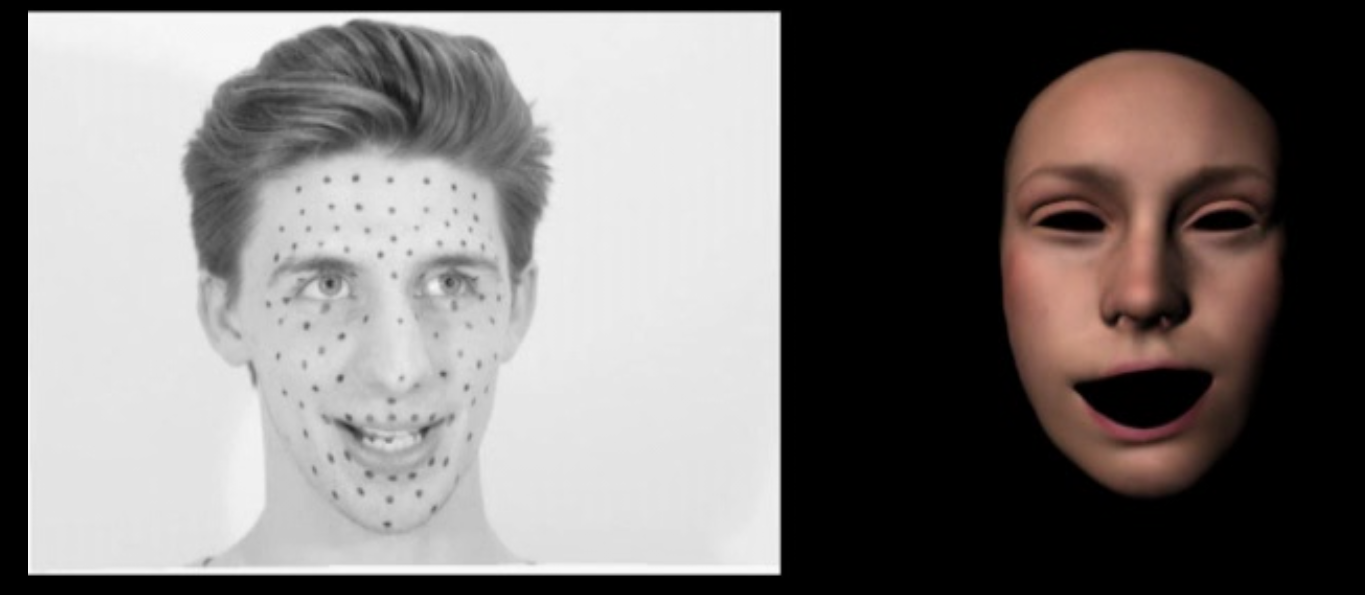
\includegraphics[width=\textwidth]{img/ghost1.png}
        \end{subfigure}
        \begin{subfigure}[b]{0.45\textwidth}
                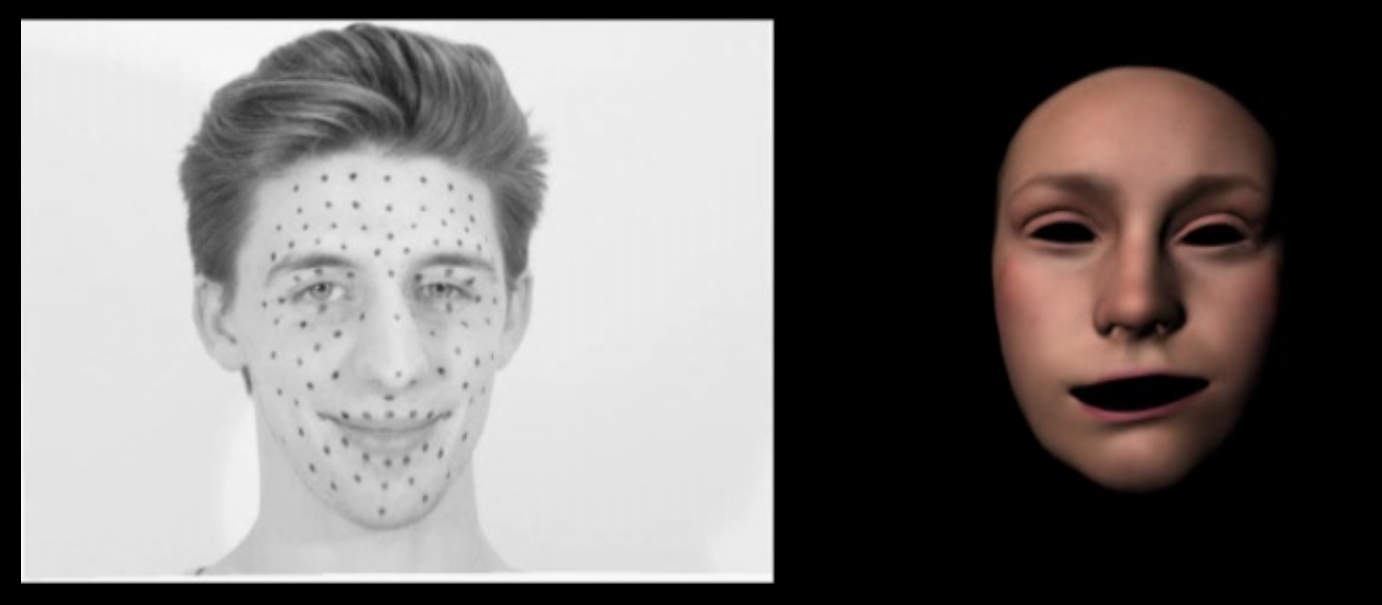
\includegraphics[width=\textwidth]{img/ghost2.png}
        \end{subfigure}
        \caption{Our first animation produced by warping the ector's expressions at each frame of the sequence. }\label{fig:ghost}
\end{figure}

\subsubsection{Introduction of Blendshapes}
In an attempt to improve the visual quality of the generated animation, we decided to use a set of Emily key-shapes, that were readily available to us. The main argument for using these blendshapes is that in most situations a simple linear relation exists between an arbitrary facial expression and the set of key-shapes. The shape may encode the entire geometry of the case, the displacement from the neutral face, or the local features of a face. If no such shapes are available, they may be producing using PCA. Such set of blendshapes is orthogonal, thus the features encoded by each shape are controlled independently; however, such shapes do not allow for intuitive facial transformations making it difficult to perform manual post-process editing.

Let us define a set of blendshapes $\mathbf{B} = [\bb_0, \ldots, \bb_n]$ where $\bb_0$ is the mesh of a neutral face, and each of the $\bb_i$ correspond to a basic facial expression, for example the raise of an eyebrow. Unless stated otherwise, we shall use $68$ shapes provided with the digital Emily model. Then a new facial expression $\mathbf{F(\w)}$ may be constructed by finding an appropriate linear combination of the offsets of the basic shapes:
\begin{equation}
	\F(\w) = \bb_0 + \sum_{i=1}^N w_i \: |\bb_i - \bb_0|, \label{eq:blendshapes}
\end{equation} where $\w = [w_1, \ldots, w_n]$ is a set of weights that describe how much each of the basic shapes affect the new expression $\mathbf{F(\w)}$. Typically, a convexity constraint is imposed on the weights; in our case the choice of constraints is influenced by the constraints present in our blendshape model, i.e. $w_i \in [0,1]$. Eq.~\ref{eq:blendshapes} may be written as a linear system of equations as follows:
\begin{equation}
	\F(\w) - \bb_0 = \hat{\mathbf{B}} \w, \label{eq:linsyst}
\end{equation} where $\hat{\mathbf{B}}$ is the original set of blendshapes without the neutral expression. 

A number of different numerical optimisation methods where tested when solving for the blendshape weights. An unconstrained solution may be calculated by inverting matrix $\hat{\mathbf{B}}$, and multiplying it from the left with the left hand side of Eq.~\ref{eq:linsyst}. Instead we use Matlab's constrained non-negative least-squares solver (\texttt{lsqnonneg}) and constrained linear least-squares solver (\texttt{lsqlin})~\cite{Matlab}. For the non-negative least-squares solver we formulate our problem as follows:
\begin{equation}
	\min_\w \| \hat{\mathbf{B}} \w - (\F(\w) - \bb_0) \|_2^2, \: \w_i \geq 0, \: i = 1, \ldots, n. \label{eq:lsqnonneg}
\end{equation} The solver uses an active set method, and iteratively improves the active set of basis vectors; it converges in finite time. The same formulation is used for the linear least squares solver though it includes an additional upper limit on the argument. This solver uses a reflexive Newton method which is able to accurately locate the local minimisers of large systems, and exhibits global convergence. It is also able to maintain sparsity of matrices but is generally slower.

\subsubsection{Two-dimensional Sequence}

Our initial tests of the optimisation algorithms were carried out on a two-dimensional sequence of facial motion. Approximately $90$ points on a sequence were marked and tracked to produce a sparse motion sequence. Then a set of key frames were hand-picked to represent the extreme cases of the facial motion, see Fig.~\ref{fig:2Dblends}. The sparse points from these frames are then used as blendshapes. The two solvers were tested on the entire motion sequence. We shall compare the results by estimating the average error between the pixels in the original sequence and the weighted sequence.

Fig.~\ref{fig:frame10} and Fig.~\ref{fig:frame400} illustrate the concept of blendshapes. Frame $10$ is very close to one of the blendshapes, and both optimisation methods are able to represent this expression well; the average error associated with the constrained non-negative least-squares solver is less than $0.29$, which corresponds to approximately $0.01$ centimetres, while the average error for the second solver is less than $0.21$ or approximately $0.09$ centimetres. Note that as expected both methods use frame $9$ with a large weight. However, the other blendshapes are different for the two methods. This suggests that none of the blendshapes is able to capture the subtle change between frames $9$ and $10$. In comparison, frame $400$ is twelve frames away from a frame that was chosen as a blendshape, resulting in an increase in average error for the two methods (approximately 0.49 in both cases). As expected, both methods use the two blendshapes that are the nearest to frame $400$ in terms of timing. The weights used for these two shapes are the same to three significant digits, and the extra shape used by the first method has a low weight assigned to it. Note that the first method does not obey the restriction of $\sum_{i=1}^N w_i = 1$. Though the second method is able to produce slightly more accurate results, at least for this data set the difference does not seem significant. 

\begin{figure}[htbp!]
\centering
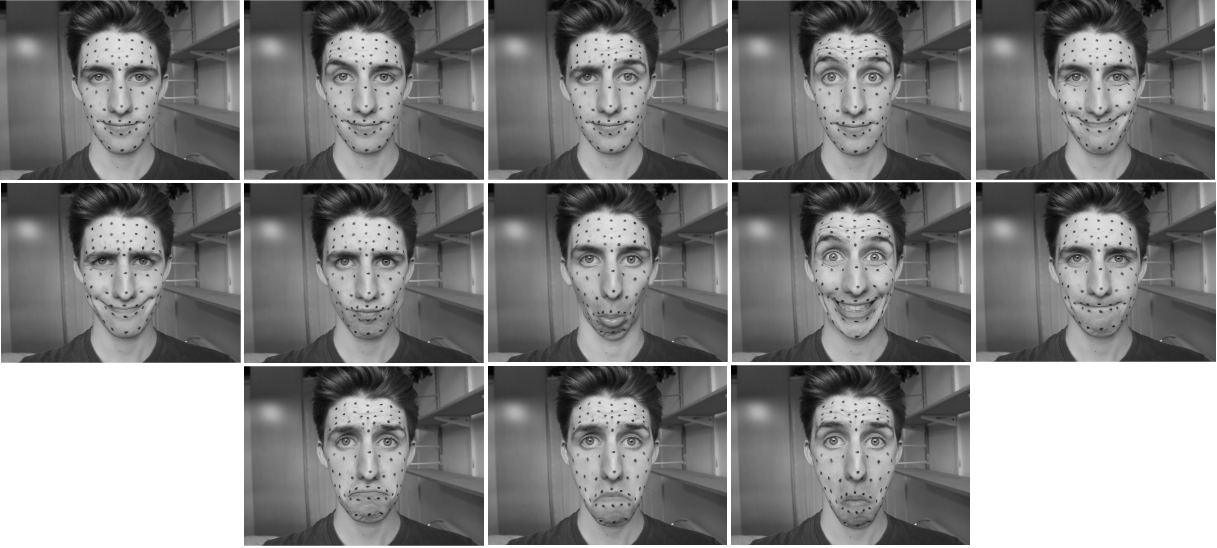
\includegraphics[width=0.8\textwidth]{img/weights/2D/basis/all.png}
	\caption{Set of facial expressions used as blendshapes. The first frame is used as a neutral expression.}
	\label{fig:2Dblends}
\end{figure}
\begin{figure}[htbp!]
\centering
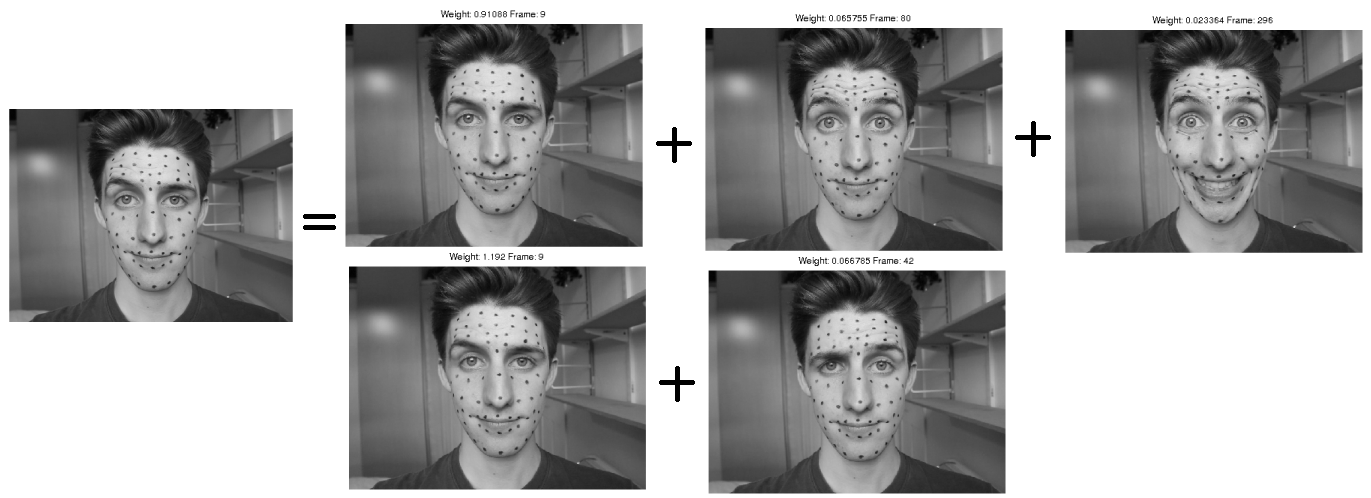
\includegraphics[width=0.8\textwidth]{img/weights/2D/frame_10/all.png}
	\caption{Frame $9$ on the left represented as a linear combination of the key frames. The top solution was obtained using the \texttt{lsqnonneg} solver while the bottom one was obtained using \texttt{lsqlin}.}
	\label{fig:frame10}
\end{figure}

\begin{figure}[htbp!]
\centering
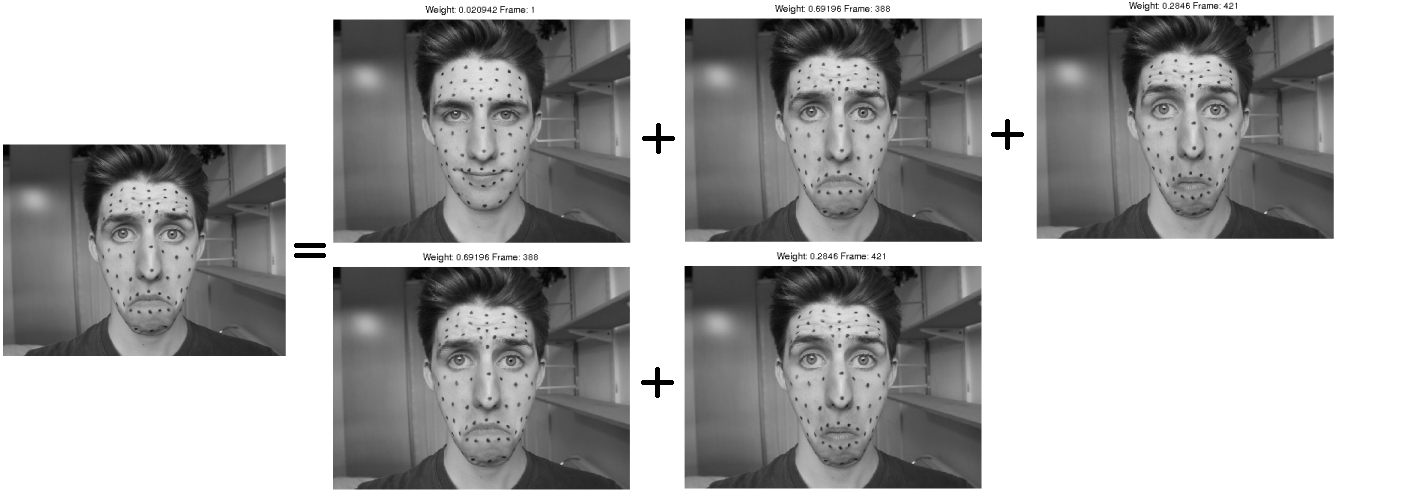
\includegraphics[width=0.8\textwidth]{img/weights/2D/frame_400/all.png}
	\caption{Frame $400$ on the left represented as a linear combination of the key frames. The top solution was obtained using the \texttt{lsqnonneg} solver while the bottom one was obtained using \texttt{lsqlin}.}
	\label{fig:frame400}
\end{figure}
\subsubsection{Principal Component Analysis}

An alternative set of key shapes may be constructed by applying Principal Component Analysis (PCA) to the observed high-dimensional data. Generally, PCA is used to transform a set of correlated observations into a set of values of linearly uncorrelated principal components. If the number of principal components is smaller than the number of original variables, then the method may be used for dimensionality reduction. PCA tries to find a set of orthonormal axes which under projection preserve the highest variance. When formulated as an eigenvalue problem, it finds the eigenvectors of the covariance matrix with the largest eigenvalues. 

PCA has been used in facial animation as an automatic way of constructing a set of blendshapes, see Sec.~\ref{sec:prfacialanimation}. The main advantages of using such blendshapes is that the construction does not require artistic skills, and the shapes are guaranteed to be orthogonal to each other. The second argument is particularly important in compression algorithms, i.e. when the aim is to find the smallest possible set of blendshapes that is able to represent the data while minimising the squared reconstruction error. We use the Matlab implementation of PCA to find a set of PCA eigenvectors that represent the directions with highest variance in our data. Given this new set of shapes, we use the same optimisation algorithm as previously described, replacing the neutral expression with the mean of the data.

To compare the results with a different number of blendshapes, we calculate the average reconstruction error for a $500$ frame sequence. When the first $3$ shapes are used, the error is approximately $0.16$ centimetres and $0.25$ centimetres for the two optimisation methods respectively. Introduction of five additional shapes reduces the error by approximately $0.02$ centimetres. Thus PCA does not outperform the model with manually designed set of key shapes. An additional drawback of the PCA basis is that it is not intuitive, i.e. the key shapes do not correspond to recognisable facial expressions. As a consequence, manual editing of the resulting animation is very complicated. Throughout the rest of the project we use the standard set of $68$ blendshapes from the Digital Emily project.

\subsubsection{Animation of a 3D Model}

Next, we shall consider the animation of the previously introduced three dimensional motion sequence. The captured sequence contains $371$ frames and shows the actor talking from approximately $12$ seconds. The corresponding sequence in the Emily domain is obtained using a linear elasticity method, see Sec.~\ref{sec:tps}. We use a talking sequence that contains $371$ frames. As in the two-dimensional case, at each frame of the sequence, the chosen optimisation method calculates the best possible combination of blendshape weights given the Emily motion sequence. In particular, the input sequence is a sparse sequence of the motion that was transformed from the capture space to the digital model space. 

We start by manually marking the three-dimensional face of Emily; we try to replicate the pattern we used when capturing the actor's face, see Fig.~\ref{fig:facemarkers}. The markers are placed at the vertices of the mesh, and the indices of these vertices are used to find the location of the corresponding markers on the meshes of the blendshapes, see Fig.~\ref{fig:Emarked}. Then the optimisation methods are used to extract the best linear combination of shapes together with the corresponding weights. The average reconstruction error for the non-negative least-squares solver is approximately $0.26$ centimetres, compared to $0.23$ centimetres for the constrained linear least-squares solver, see Fig.~\ref{fig:errorw2w3}. A number of factors may increase the error. Firstly, the expressions captured in Emily blendshapes are fairly mild, i.e. the shapes do not capture the most extreme motion of the face. Consequently, the estimated facial movements may not be expressed as a linear combination of the blendshapes. Secondly, as the blendshapes are not orthogonal, they may combine in unexpected ways, for example cancel each other. This behaviour may be avoided if a set of PCA-produced shapes is used. Also, note that the mesh of Emily is not symmetrical, i.e. the left side of the face does not match the right side. This may lead to a sideways motion that cannot be captured by the blendshapes.
\begin{figure}[htbp!]
        \centering
        \begin{subfigure}[b]{0.25\textwidth}
                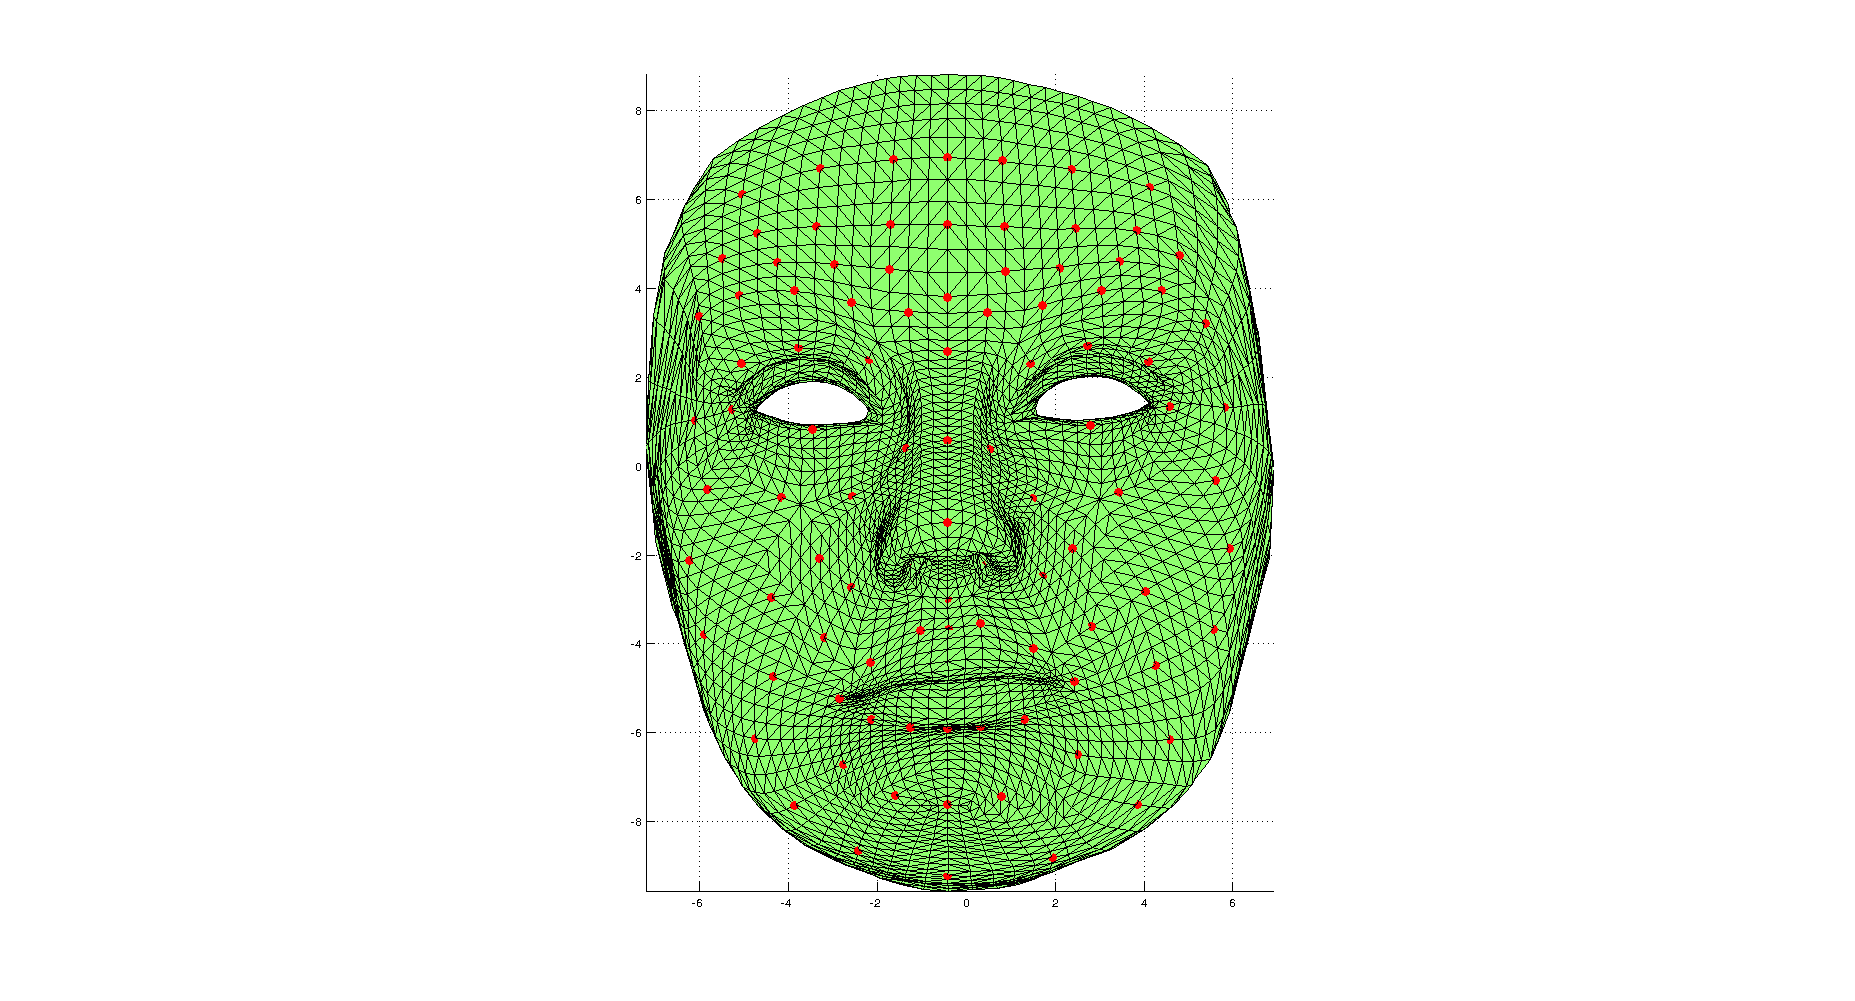
\includegraphics[trim = 160mm 20mm 160mm 10mm, clip,width=0.7\textwidth]{img/weights/3D/Emily_marked/neutralE_marked.png}
        \end{subfigure}%
        ~ %add desired spacing between images, e. g. ~, \quad, \qquad, \hfill etc.
          %(or a blank line to force the subfigure onto a new line)
        \begin{subfigure}[b]{0.25\textwidth}
                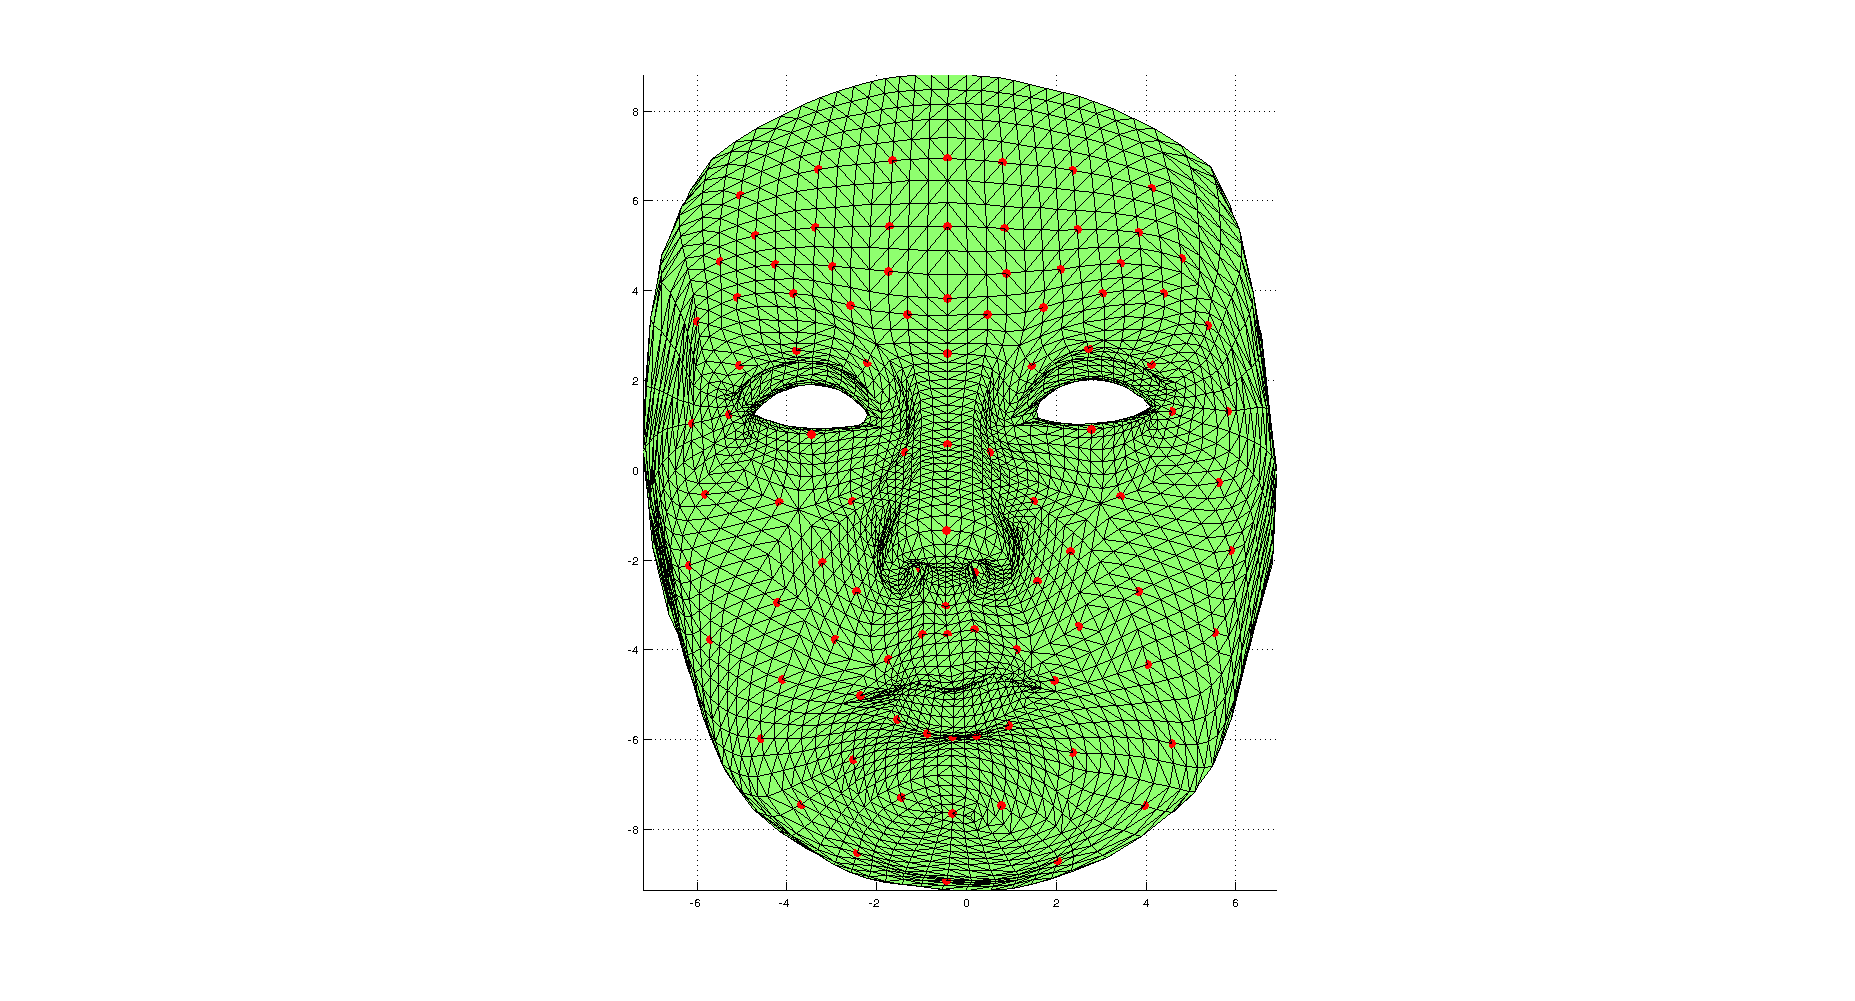
\includegraphics[trim = 160mm 20mm 160mm 10mm, clip,width=0.7\textwidth]{img/weights/3D/Emily_marked/blendshapeE_marked_50.png}
        \end{subfigure}
        ~ %add desired spacing between images, e. g. ~, \quad, \qquad, \hfill etc.
          %(or a blank line to force the subfigure onto a new line)
        \begin{subfigure}[b]{0.25\textwidth}
                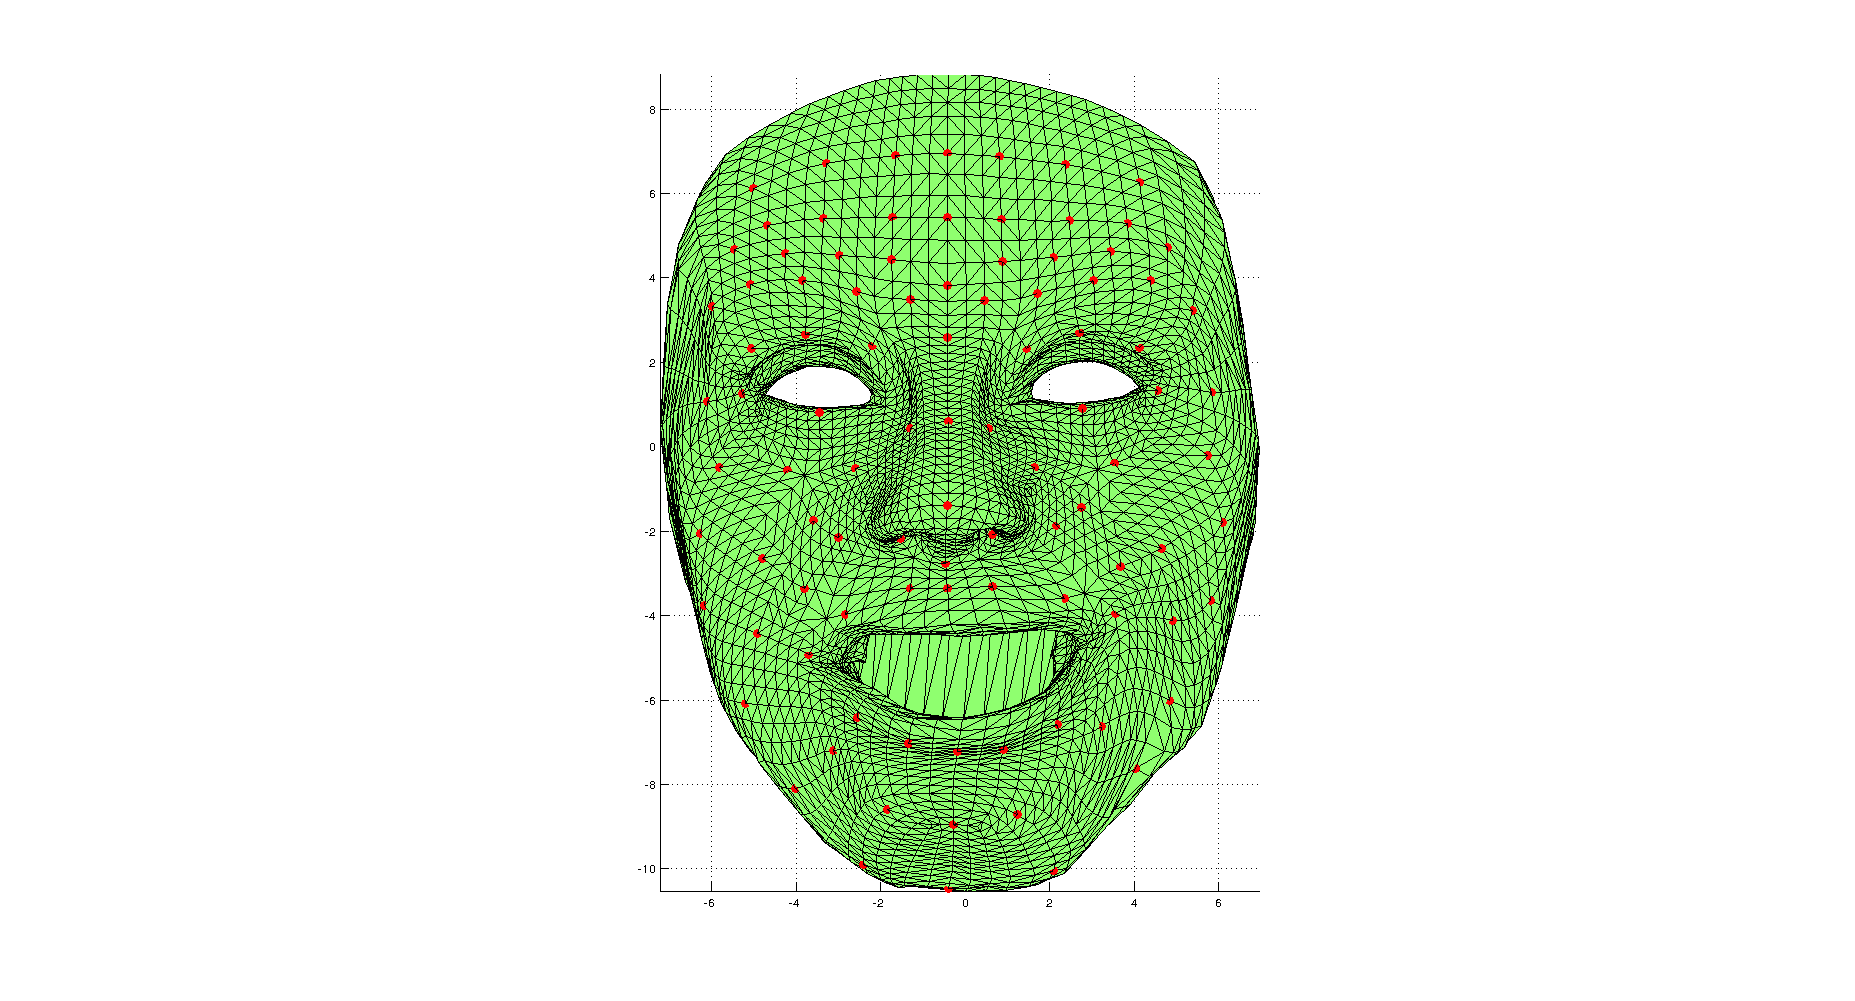
\includegraphics[trim = 160mm 20mm 160mm 10mm,clip,width=0.7\textwidth]{img/weights/3D/Emily_marked/blendshapeE_marked_56.png} 
        \end{subfigure} \\
        \begin{subfigure}[b]{0.25\textwidth}
                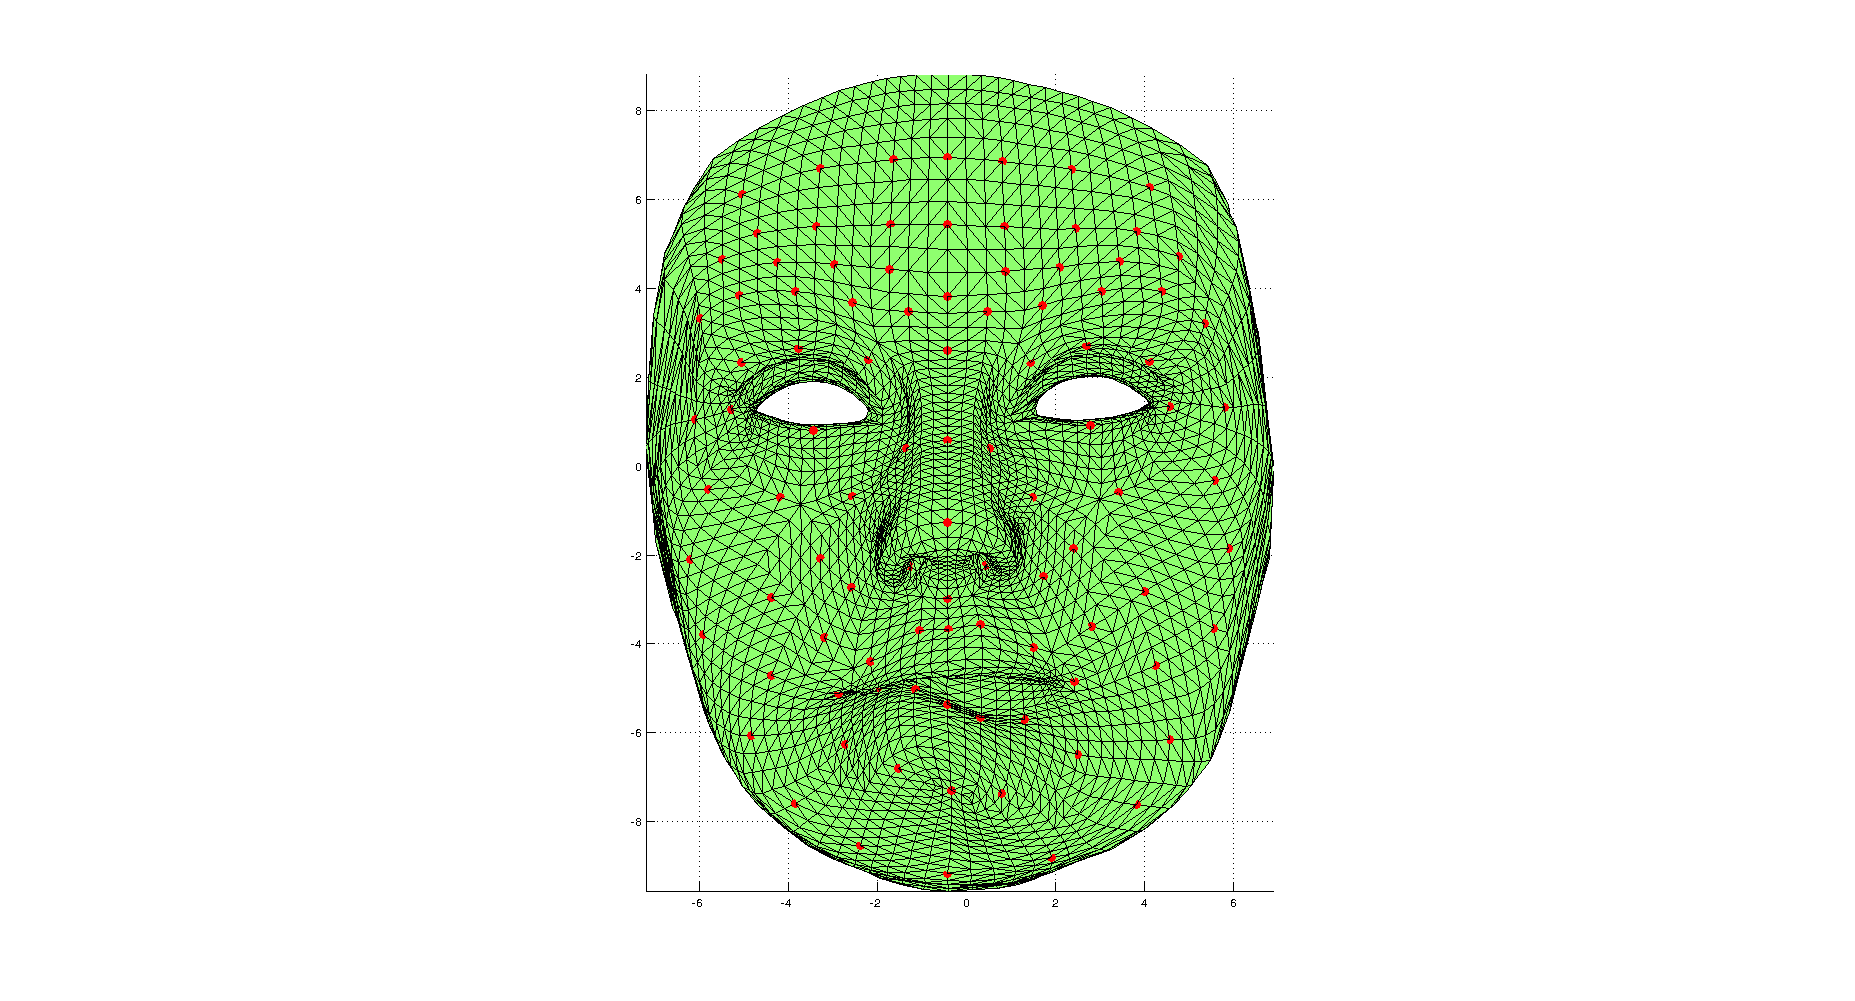
\includegraphics[trim = 160mm 20mm 160mm 10mm,clip,width=0.7\textwidth]{img/weights/3D/Emily_marked/blendshapeE_marked_61.png}
        \end{subfigure}%
        ~ %add desired spacing between images, e. g. ~, \quad, \qquad, \hfill etc.
          %(or a blank line to force the subfigure onto a new line)
        \begin{subfigure}[b]{0.25\textwidth}
                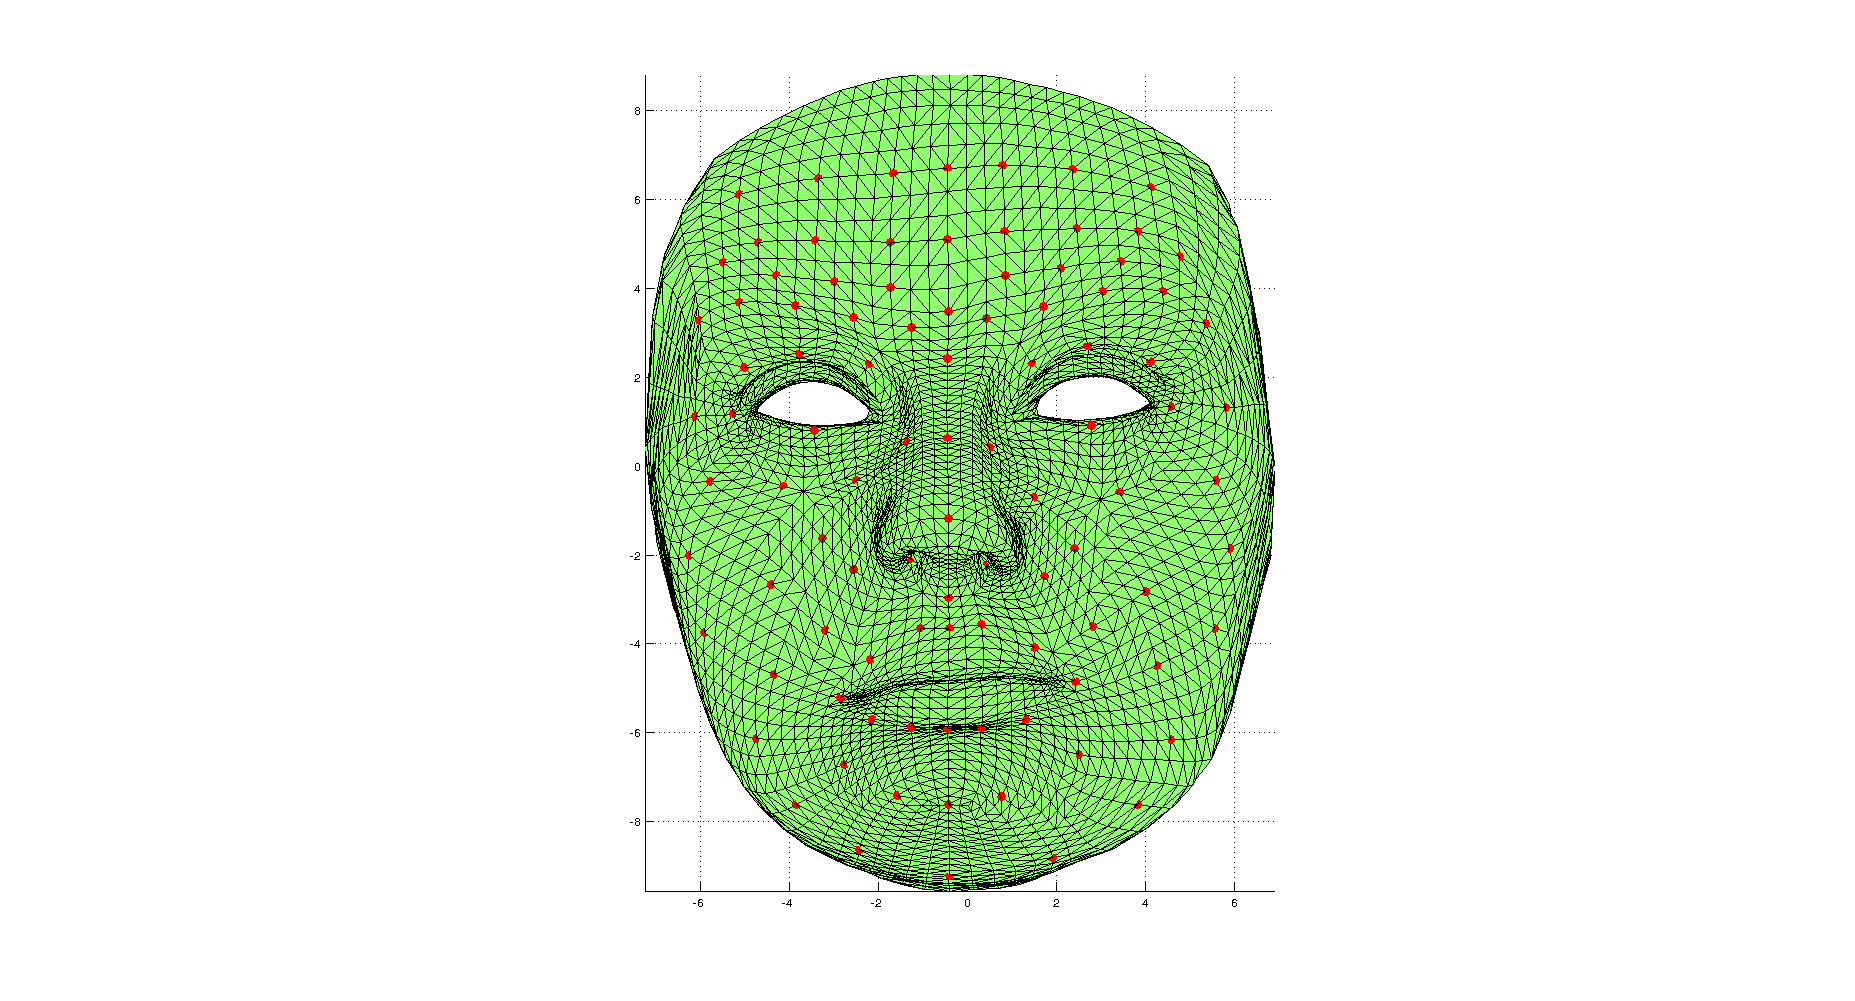
\includegraphics[trim = 160mm 20mm 160mm 10mm,clip,width=0.7\textwidth]{img/weights/3D/Emily_marked/blendshapeE_marked_67.png}
        \end{subfigure}
        ~ %add desired spacing between images, e. g. ~, \quad, \qquad, \hfill etc.
          %(or a blank line to force the subfigure onto a new line)
        \begin{subfigure}[b]{0.25\textwidth}
                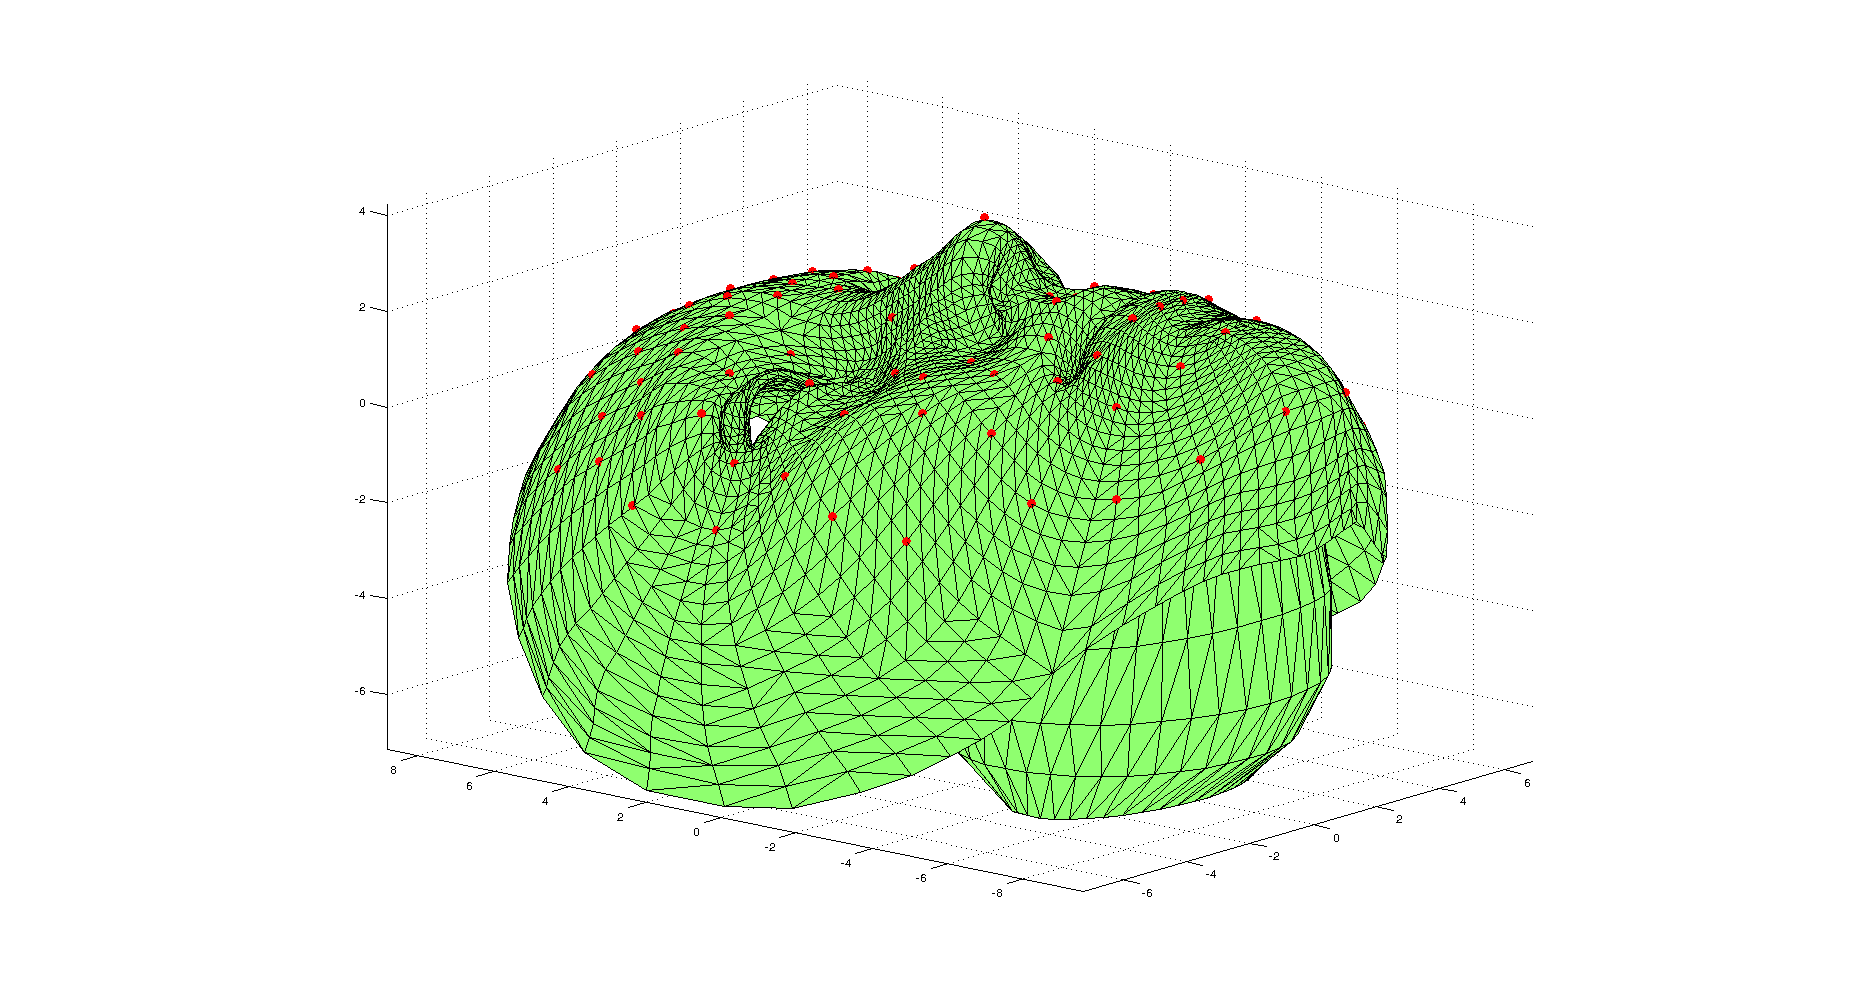
\includegraphics[trim = 120mm 20mm 120mm 10mm, clip, width=0.7\textwidth]{img/weights/3D/Emily_marked/neutralE_marked_rot.png}
        \end{subfigure}
        \caption{Examples of marked blendshapes.}\label{fig:Emarked}
\end{figure}

\begin{figure}[htbp!]
        \centering
        \begin{subfigure}[b]{0.3\textwidth}
                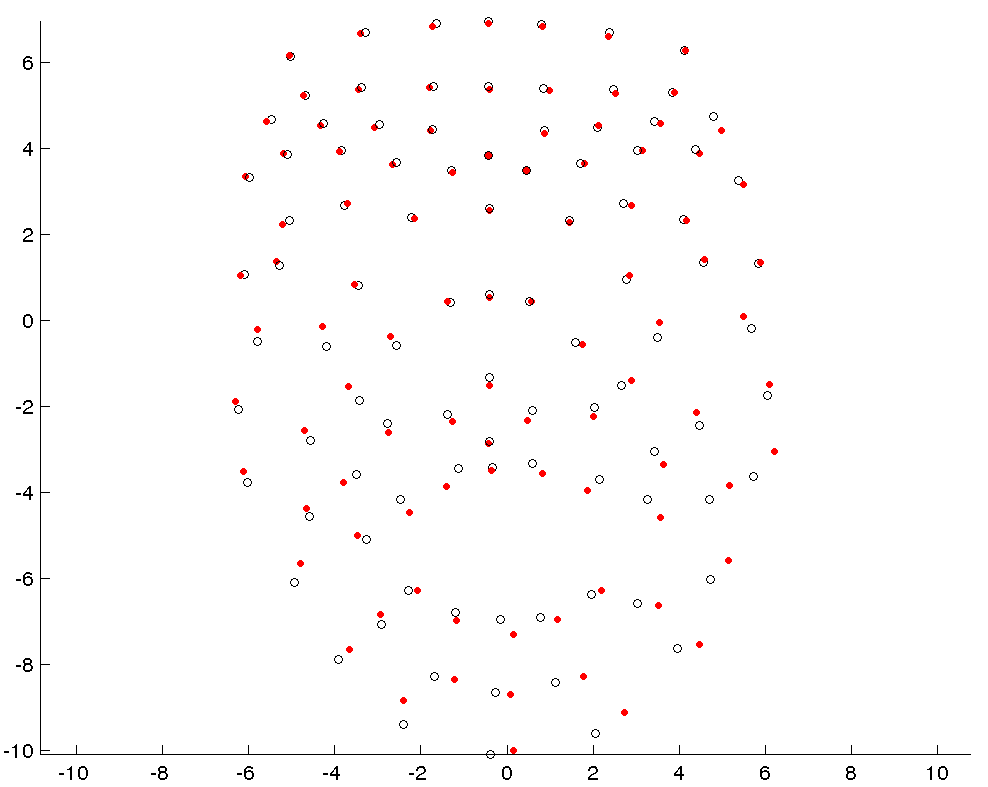
\includegraphics[width=\textwidth]{img/weights/3D/w2/w2_frame200_blends68.png}
        \end{subfigure}%
        ~ %add desired spacing between images, e. g. ~, \quad, \qquad, \hfill etc.
          %(or a blank line to force the subfigure onto a new line)
        \begin{subfigure}[b]{0.3\textwidth}
                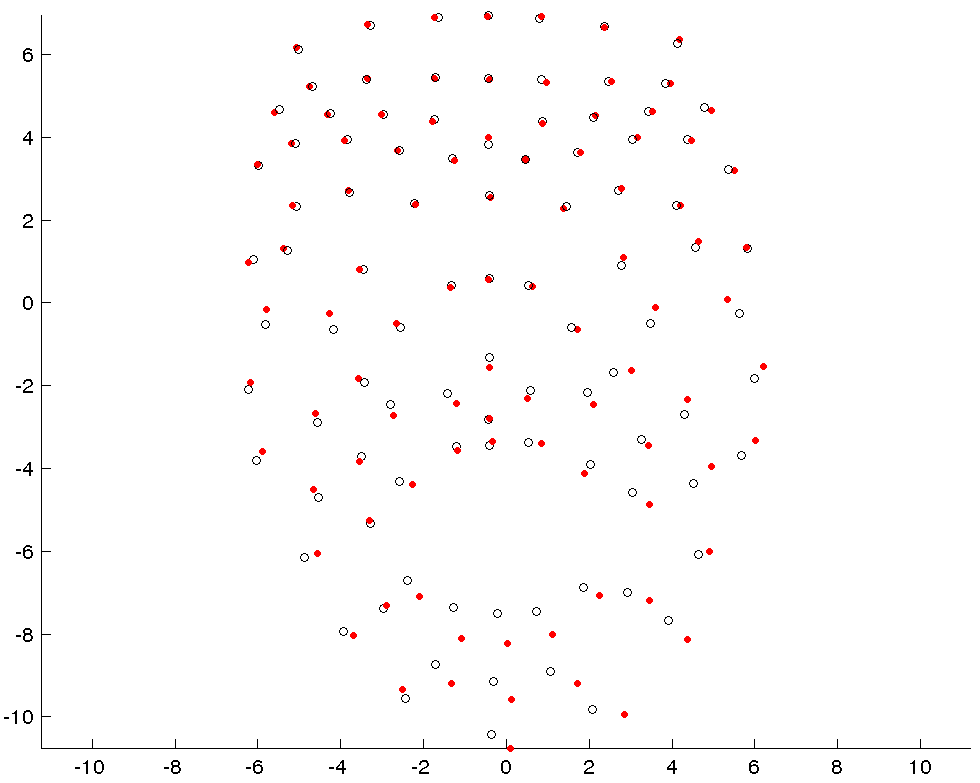
\includegraphics[width=\textwidth]{img/weights/3D/w2/w2_frame400_blends68.png}
        \end{subfigure}
        ~ %add desired spacing between images, e. g. ~, \quad, \qquad, \hfill etc.
          %(or a blank line to force the subfigure onto a new line)
        \begin{subfigure}[b]{0.3\textwidth}
                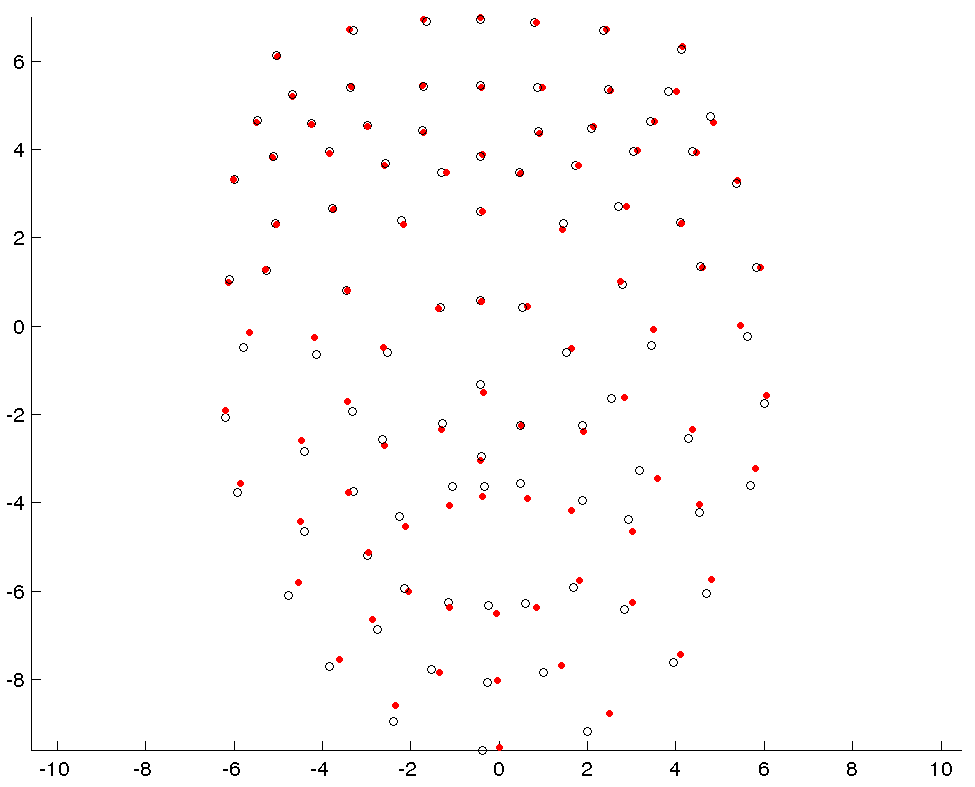
\includegraphics[width=\textwidth]{img/weights/3D/w2/w2_frame600_blends68.png} 
        \end{subfigure} \\
                \begin{subfigure}[b]{0.3\textwidth}
                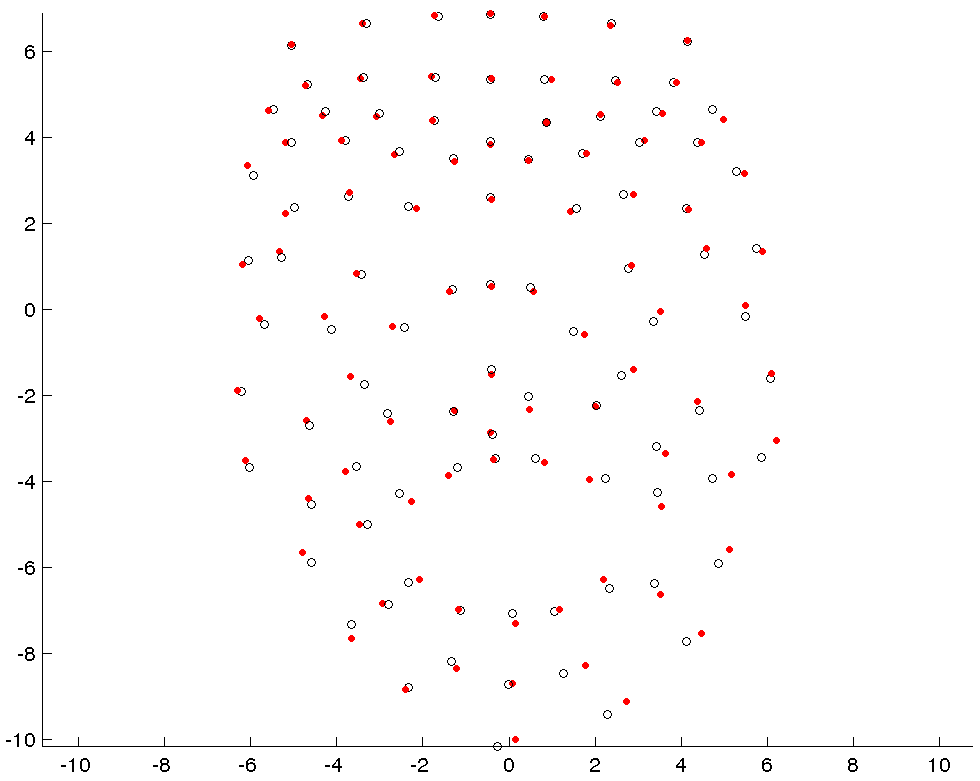
\includegraphics[width=\textwidth]{img/weights/3D/w3/w3_200.png}
        \end{subfigure}%
        ~ %add desired spacing between images, e. g. ~, \quad, \qquad, \hfill etc.
          %(or a blank line to force the subfigure onto a new line)
        \begin{subfigure}[b]{0.3\textwidth}
                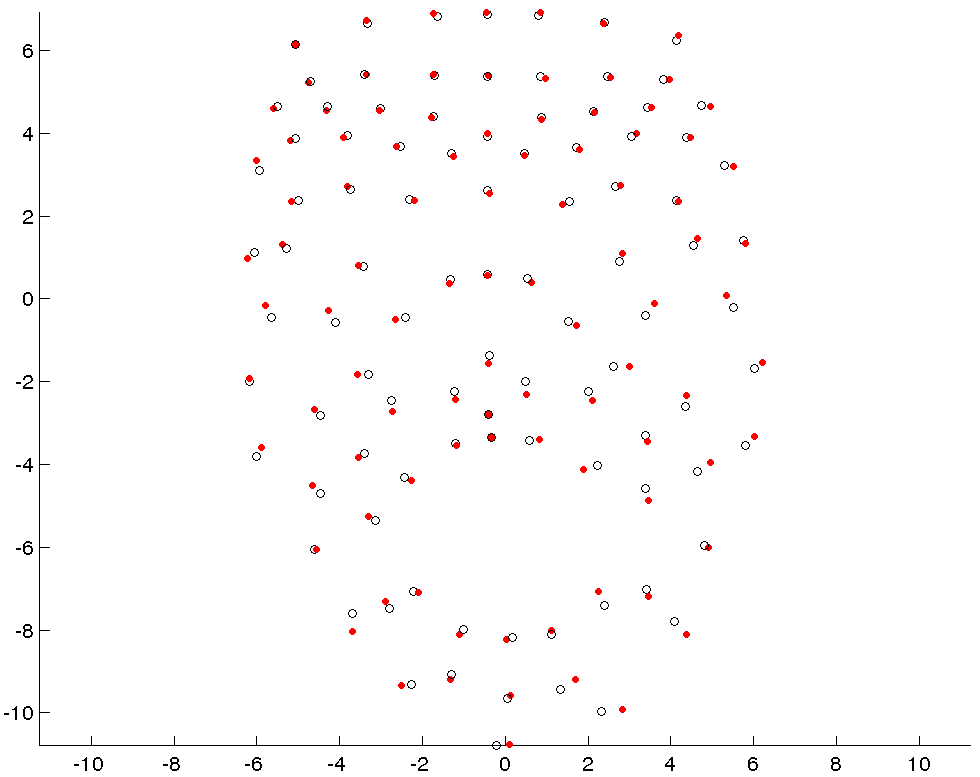
\includegraphics[width=\textwidth]{img/weights/3D/w3/w3_400.png}
        \end{subfigure}
        ~ %add desired spacing between images, e. g. ~, \quad, \qquad, \hfill etc.
          %(or a blank line to force the subfigure onto a new line)
        \begin{subfigure}[b]{0.3\textwidth}
                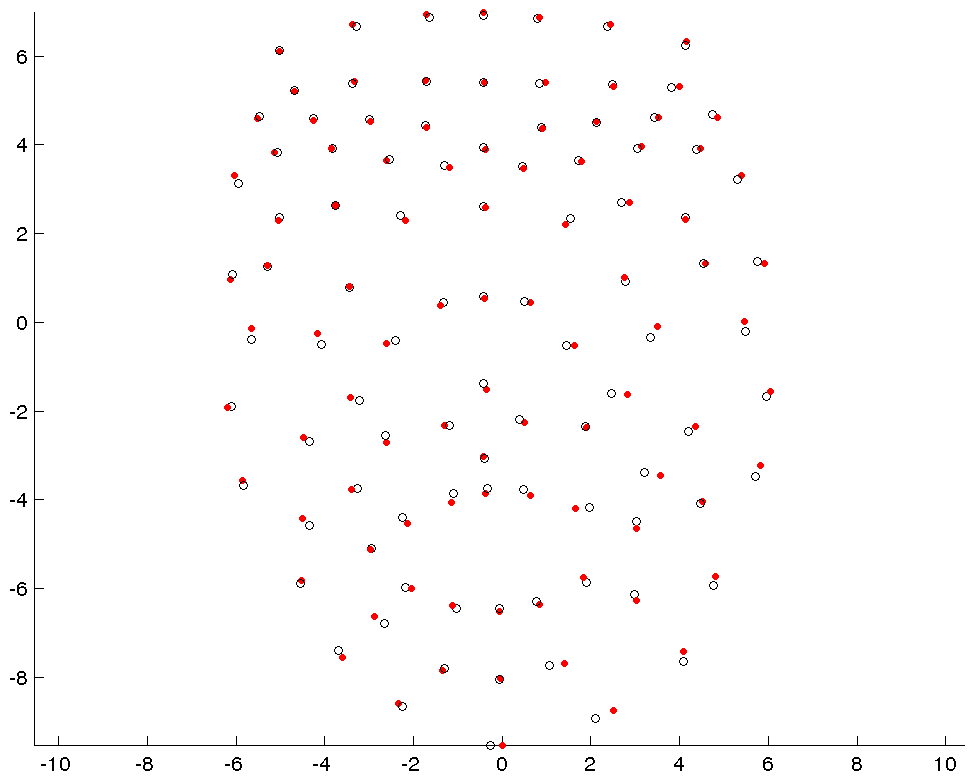
\includegraphics[width=\textwidth]{img/weights/3D/w3/w3_600.png} 
        \end{subfigure}
        \caption{The red dots mark the position of the markers in the motion sequence while the black cirles correspond to the reconstructed position of the markers. The top results were produced using the non-negative least-squares solver while the bottom results were produced by the linear least-squares solver. }\label{fig:errorw2w3}
\end{figure}

The use of blendshapes greatly improves the visual quality of the resulting animation. However, the animation still lacks realism and expressiveness, thus we implement a number of changes to the original model. Firstly, we aim to find a sparse solution, i.e. minimise the number of blendshapes used at any given time. This is done by adding a penalty term on the $L1$-norm of the weights to the original minimisation problem. Then an iterative method is used to find the optimal set of weights; we use a Matlab implementation of the LASSO algorithm~\cite{Schmidt:2005}. After careful adjustment of the scaling parameter, the least squares solver is able to reduce the mean reconstruction error by approximately $0.03$ centimetres. However, the best sparse results were achieved without imposing the upper and lower bound on the weights. We found that in our case it is more import to impose these bounds than to favour sparse solutions. Moreover, the solution produced by the constrained non-negative least squares solver uses on average $21$ blendshapes per frame, which does not seem unreasonable given the complexity of human facial motion.

As noted by Bouaziz et al., a motion capture sequence also has temporal constraints, i.e. each frame is closely related to the previous frames~\cite{Bouaziz:2013}. This constraint may be included in the minimisation problem by adding a smoothness term, $||\w^{t-2} - 2 \w^{t-1} + \w^t||^2_2$, where $\w$ is the vector of weights, and $t$ is the frame number. The resulting problem is generally hard to solve, but there exist a number of algorithms that minimise the sum of Euclidean norms. Beside the one mention in the paper by Bouaziz et al., we have considered the algorithms proposed by Andersen et al., and Xue and Ye~\cite{Andersen:2000}, ~\cite{Xue:1997}. However, after examining the solution produced by our current methods, we noticed that it automatically obeys this smoothness constraint; this may be explained by the fact that the input sequence was filmed at a relatively high frame rate ($60$ frames per second). Specifically, we compared the change in blendshape weights from frame to frame; the average difference is $0.007$, which, when reconstructed, is hardy noticeable. The highest differences (of around $0.3$) appear during the opening and closing of the mouth; these transitions look natural at the original frame rate. We note that if the motion capture data was recorded at a low frame rate, then the implementation of the temporal constraints might improve the quality of the resulting animation.

Next, we examined the effect of using a reduced set of key expressions in the solver; this leads to a smaller system of equations to be optimised. The reduced set contains $19$ shapes included in the visual set of controls in the original blendshape model. The smaller set of shapes leads to a slight increase (of approximately $0.03$ centimetres) in reconstruction error. There is no noticeable effect on the visual quality of the resulting animation, see Fig.~\ref{fig:19blends}. Thus the only notable advantage of using fewer blendshapes is the acceleration of the  optimisation step. However, if the performance of the algorithm is the main objective, then a PCA basis is a better choice than a reduced non-orthogonal set of shapes.

\begin{figure}[htbp!]
        \centering
        \begin{subfigure}[b]{0.3\textwidth}
                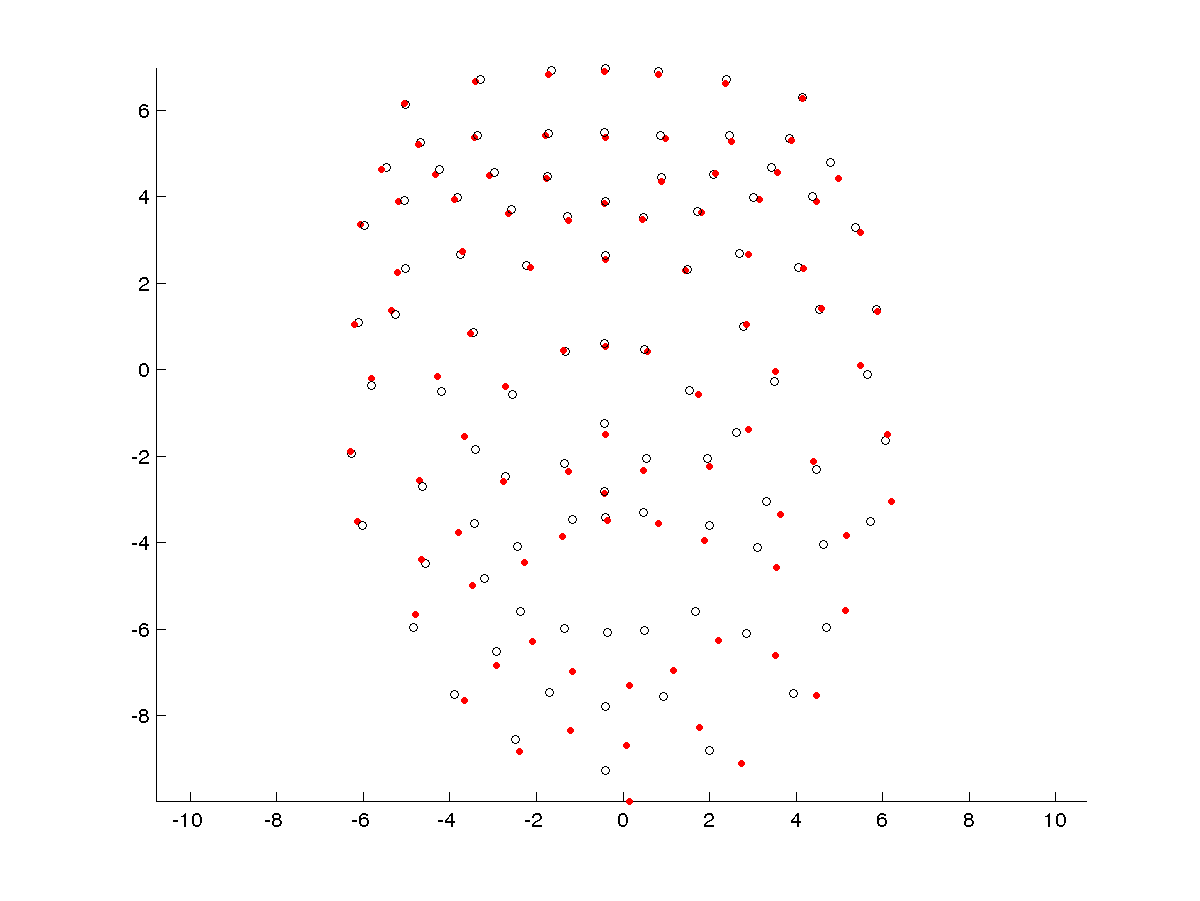
\includegraphics[trim = 10mm 0mm 10mm 0mm,clip,width=\textwidth]{img/weights/3D/19blends/w2_frame200_blends19.png}
        \end{subfigure}%
        ~ %add desired spacing between images, e. g. ~, \quad, \qquad, \hfill etc.
          %(or a blank line to force the subfigure onto a new line)
        \begin{subfigure}[b]{0.3\textwidth}
                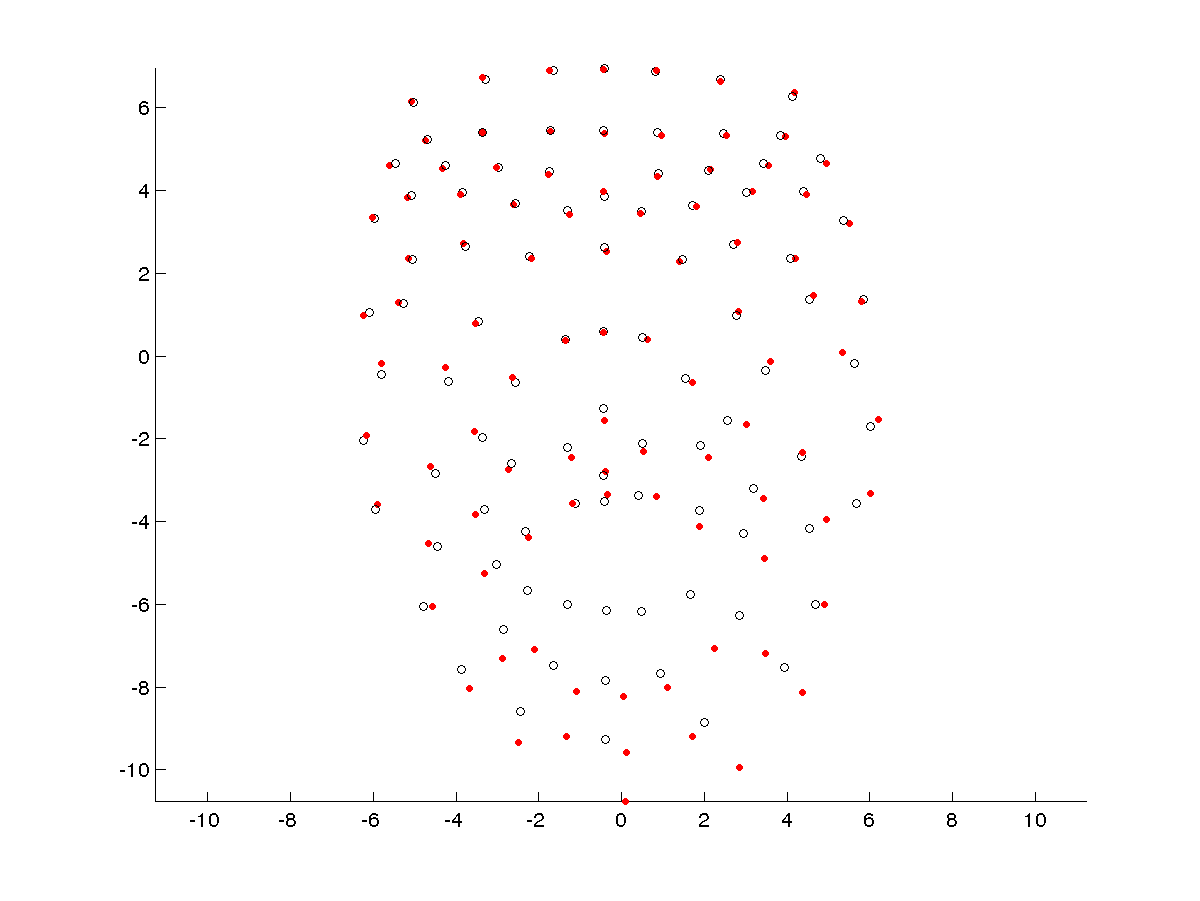
\includegraphics[trim = 10mm 0mm 10mm 0mm,clip,width=\textwidth]{img/weights/3D/19blends/w2_frame400_blends19.png}
        \end{subfigure}
        ~ %add desired spacing between images, e. g. ~, \quad, \qquad, \hfill etc.
          %(or a blank line to force the subfigure onto a new line)
        \begin{subfigure}[b]{0.3\textwidth}
                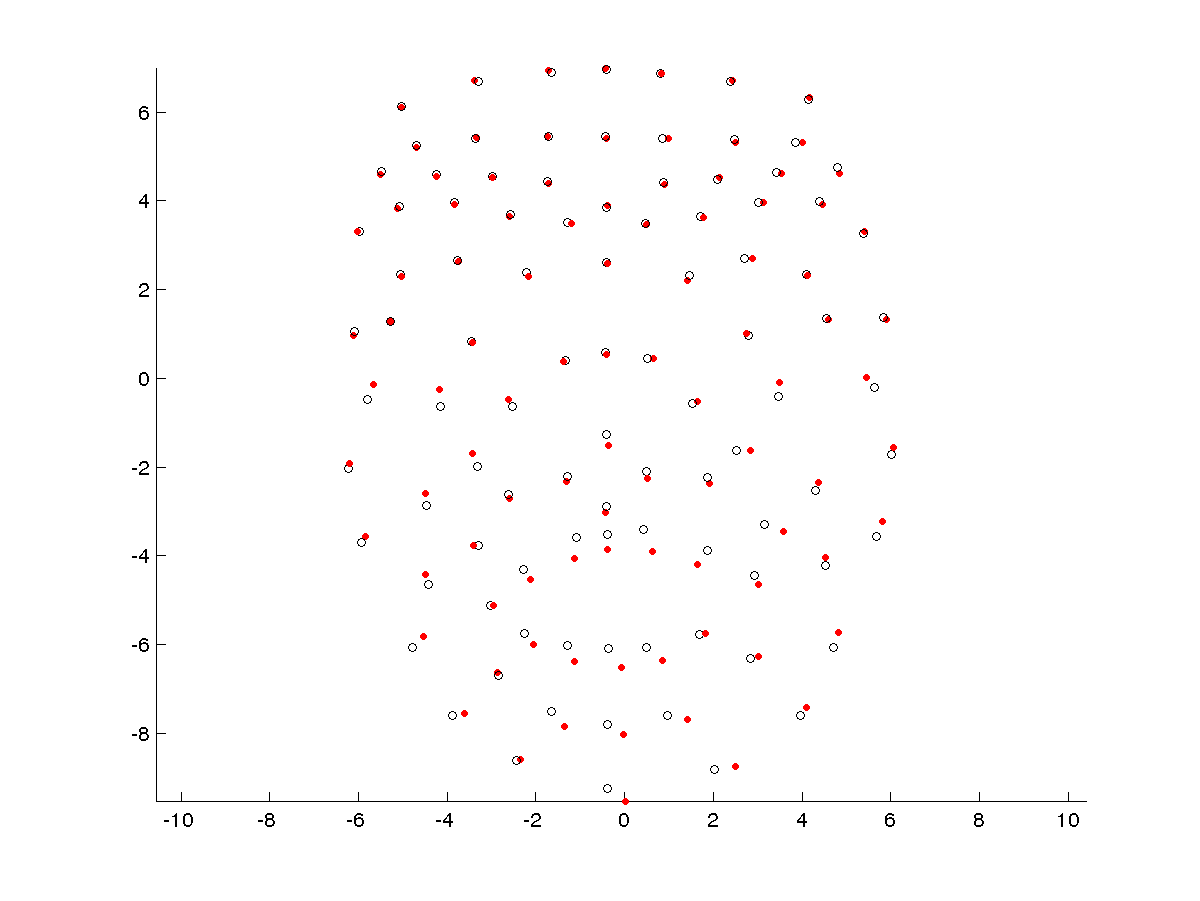
\includegraphics[trim = 10mm 0mm 10mm 0mm,clip,width=\textwidth]{img/weights/3D/19blends/w2_frame600_blends19.png} 
        \end{subfigure} \\
        \begin{subfigure}[b]{0.3\textwidth}
                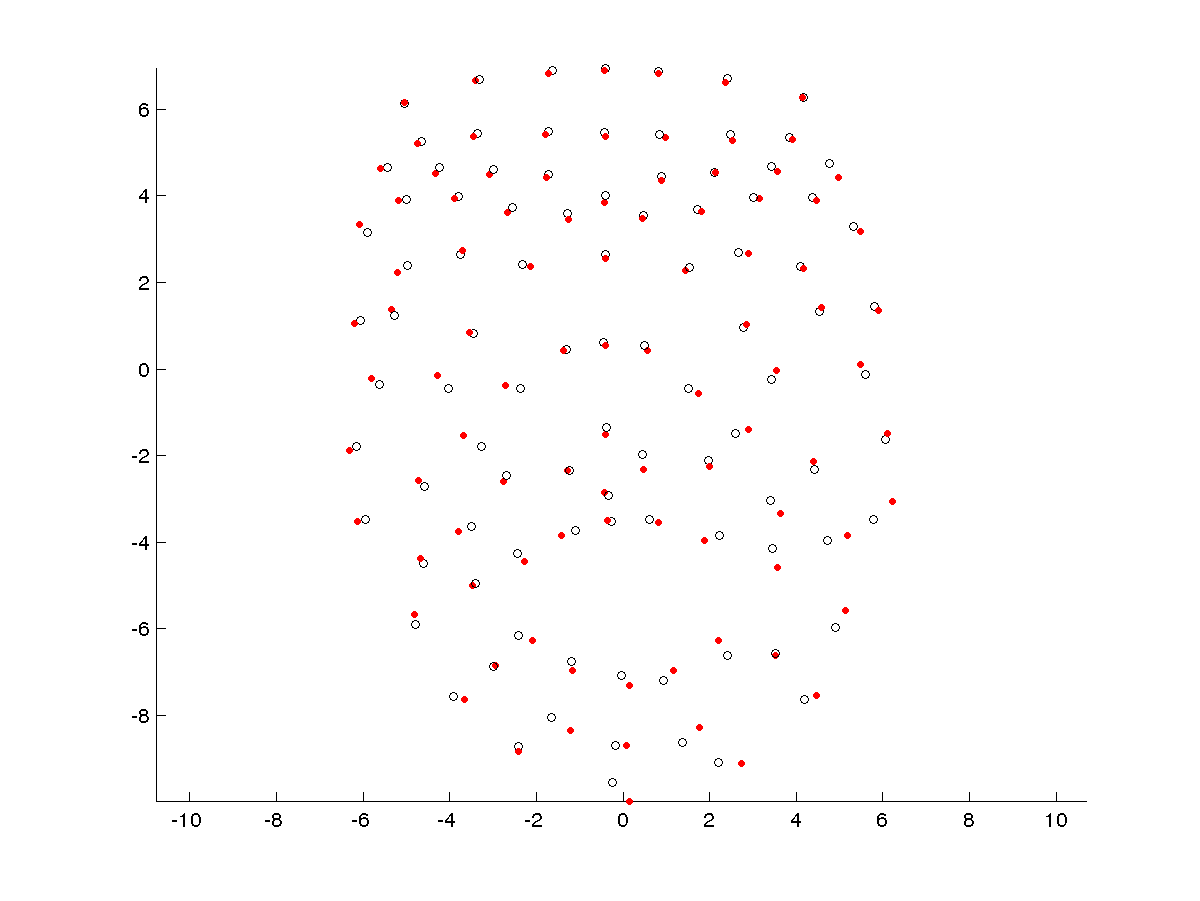
\includegraphics[trim = 10mm 0mm 10mm 0mm,clip,width=\textwidth]{img/weights/3D/19blends/w3_frame200_blends19.png}
        \end{subfigure}%
        ~ %add desired spacing between images, e. g. ~, \quad, \qquad, \hfill etc.
          %(or a blank line to force the subfigure onto a new line)
        \begin{subfigure}[b]{0.3\textwidth}
                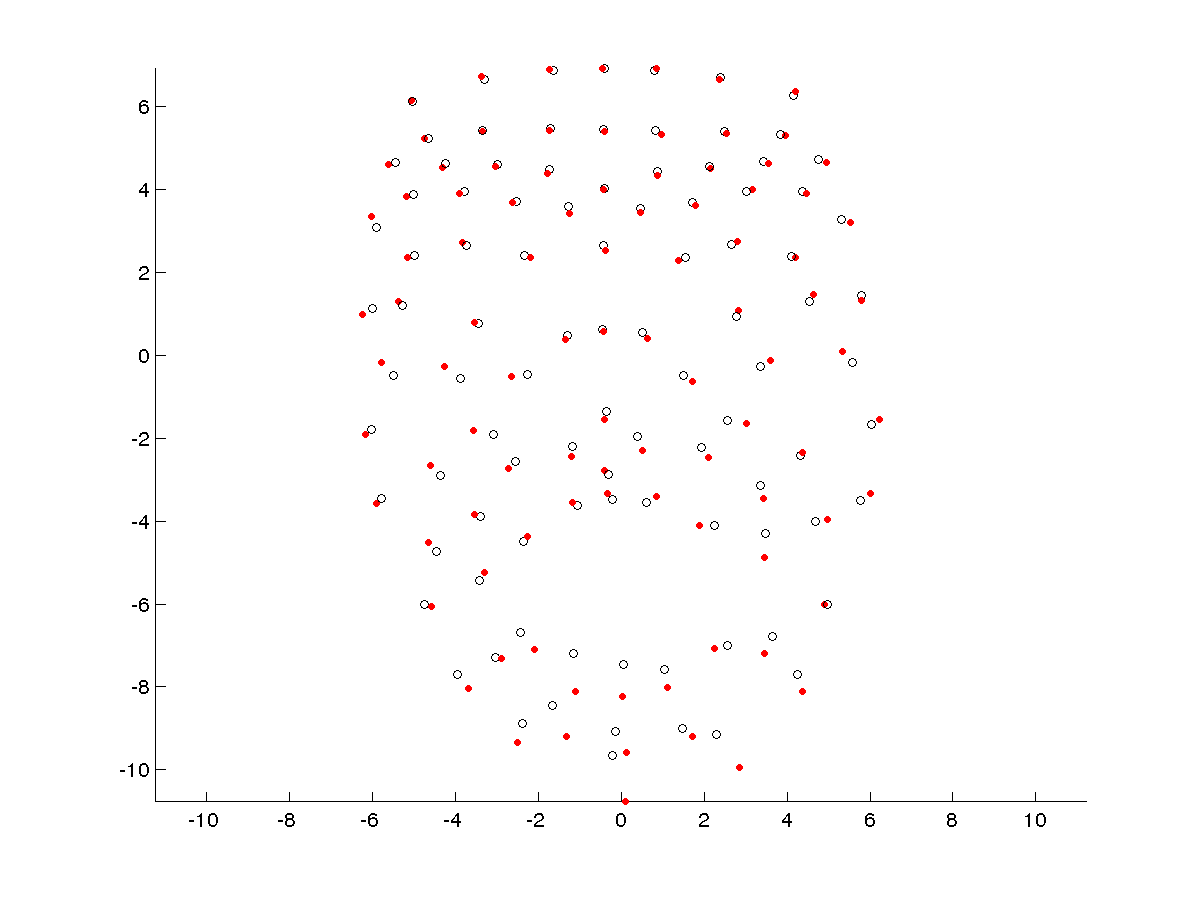
\includegraphics[trim = 10mm 0mm 10mm 0mm,clip,width=\textwidth]{img/weights/3D/19blends/w3_frame400_blends19.png}
        \end{subfigure}
        ~ %add desired spacing between images, e. g. ~, \quad, \qquad, \hfill etc.
          %(or a blank line to force the subfigure onto a new line)
        \begin{subfigure}[b]{0.3\textwidth}
                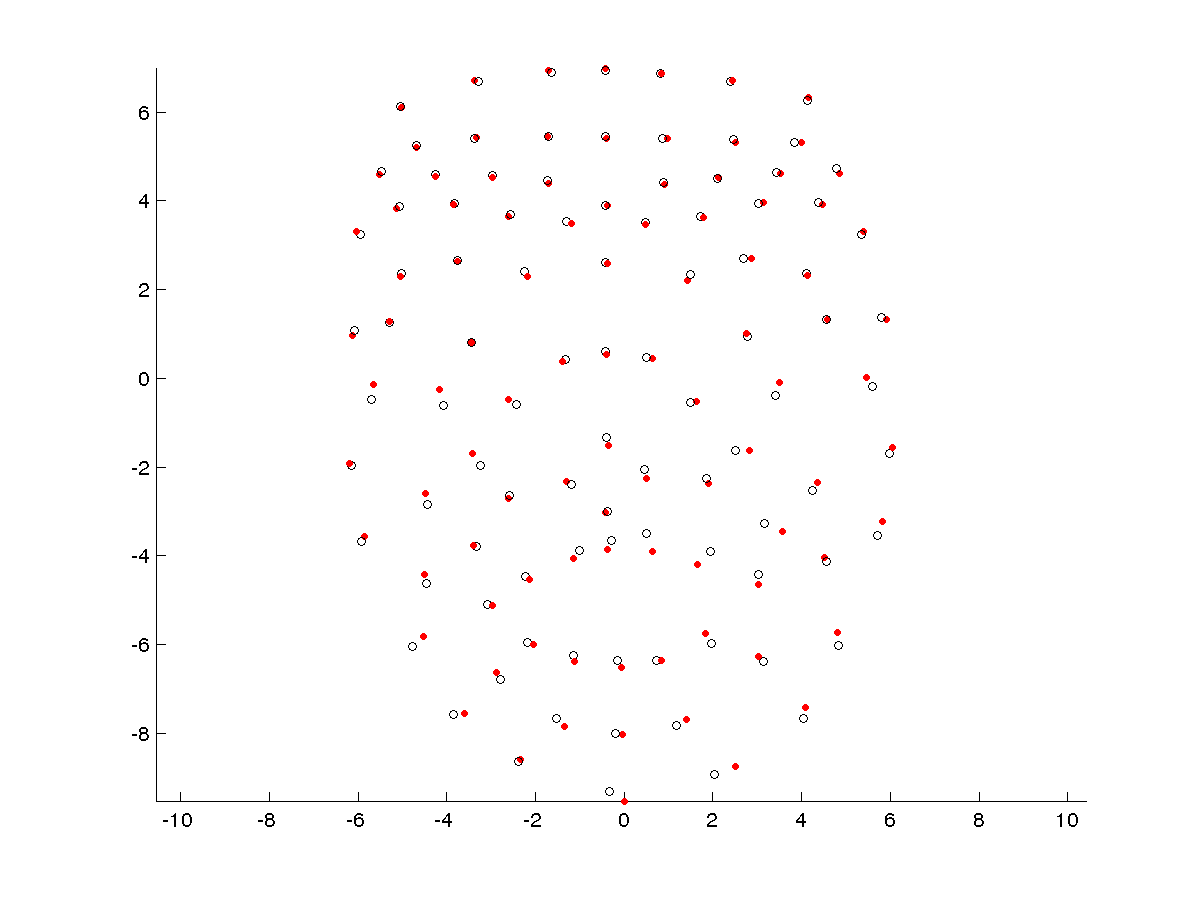
\includegraphics[trim = 10mm 0mm 10mm 0mm,clip,width=\textwidth]{img/weights/3D/19blends/w3_frame600_blends19.png} 
        \end{subfigure}
        \caption{The reconstruction error for a model with $19$ blendshapes. The top results were produced using the non-negative least-squares solver while the bottom results were produced by the linear least-squares solver. Colours as in Fig.~\ref{fig:errorw2w3}.}\label{fig:19blends}
\end{figure}

For comparison, we attempt the opposite approach; we include extra blendshapes to account for the features that are not present in the original set. This approach was inspired by the research of Li et al., who introduced corrective shapes to systematically extend the initial set of shapes~\cite{Li:2013}. The authors start by using linear combinations of PCA principal components to construct new facial expressions. They then extract a number of samples that cannot be explained by the original set of principal components. An iterative procedure is used to produce corrective shapes that are orthogonal to the members of the original set, and that improve the fitting accuracy. Unfortunately, such corrective method cannot be applied to a manually constructed set of blendshapes since it relies on vector orthogonality. Instead, we manually construct a set of new shapes that are more extreme than our original blendshapes; we then include these new shapes in the solver. The criteria for choosing the new expressions are, (a) the likelihood of that or similar expressions, and (b) the dissimilarity of the new expressions in comparison to the existing ones. The four extra blendshapes are shown in Fig.~\ref{fig:extrafaces}; they were constructed by increasing the weights on the original blendshapes beyond the predefined limit. 
\begin{figure}[htbp!]
        \centering
        \begin{subfigure}[b]{0.23\textwidth}
                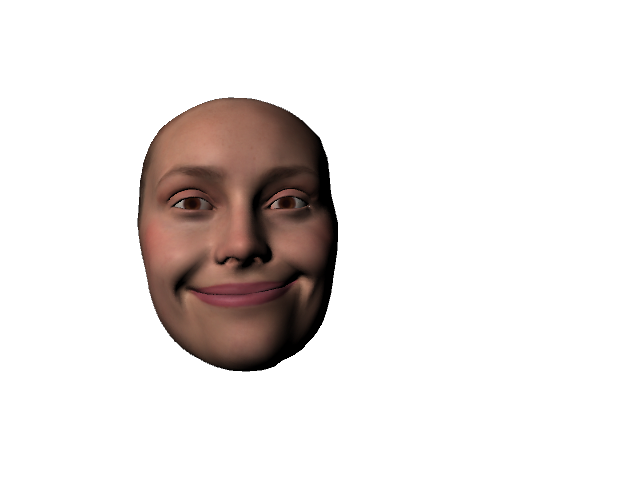
\includegraphics[trim = 50mm 30mm 80mm 30mm,clip,width=\textwidth]{img/weights/3D/Extrafaces/lipcorners15.png}
        \end{subfigure}
        ~ %add desired spacing between images, e. g. ~, \quad, \qquad, \hfill etc.
          %(or a blank line to force the subfigure onto a new line)
        \begin{subfigure}[b]{0.23\textwidth}
                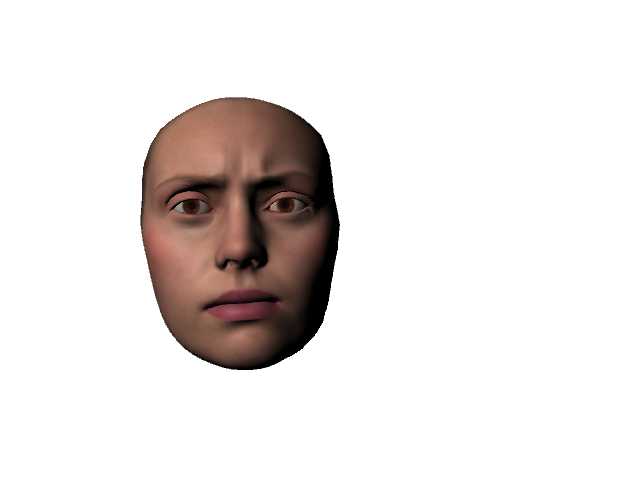
\includegraphics[trim = 50mm 30mm 80mm 30mm,clip,width=\textwidth]{img/weights/3D/Extrafaces/eyebrowsin2.png}
        \end{subfigure} 
        \begin{subfigure}[b]{0.23\textwidth}
                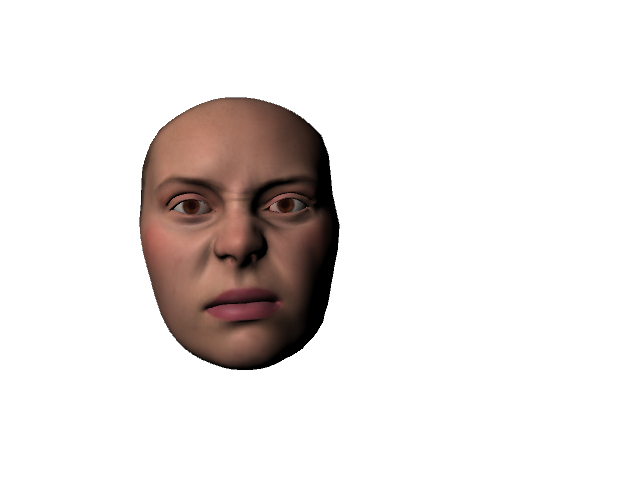
\includegraphics[trim = 50mm 30mm 80mm 30mm,clip,width=\textwidth]{img/weights/3D/Extrafaces/nosewrinkle2.png}
        \end{subfigure}
        ~ %add desired spacing between images, e. g. ~, \quad, \qquad, \hfill etc.
          %(or a blank line to force the subfigure onto a new line)
        \begin{subfigure}[b]{0.23\textwidth}
                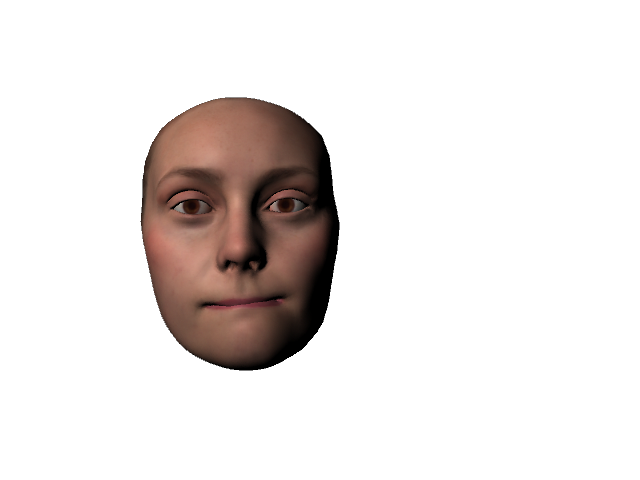
\includegraphics[trim = 50mm 30mm 80mm 30mm,clip,width=\textwidth]{img/weights/3D/Extrafaces/mouthsuck.png}
        \end{subfigure}
        \caption{Additional blendshapes. }\label{fig:extrafaces}
\end{figure}
\begin{figure}[htbp!]
        \centering
        \begin{subfigure}[b]{0.47\textwidth}
                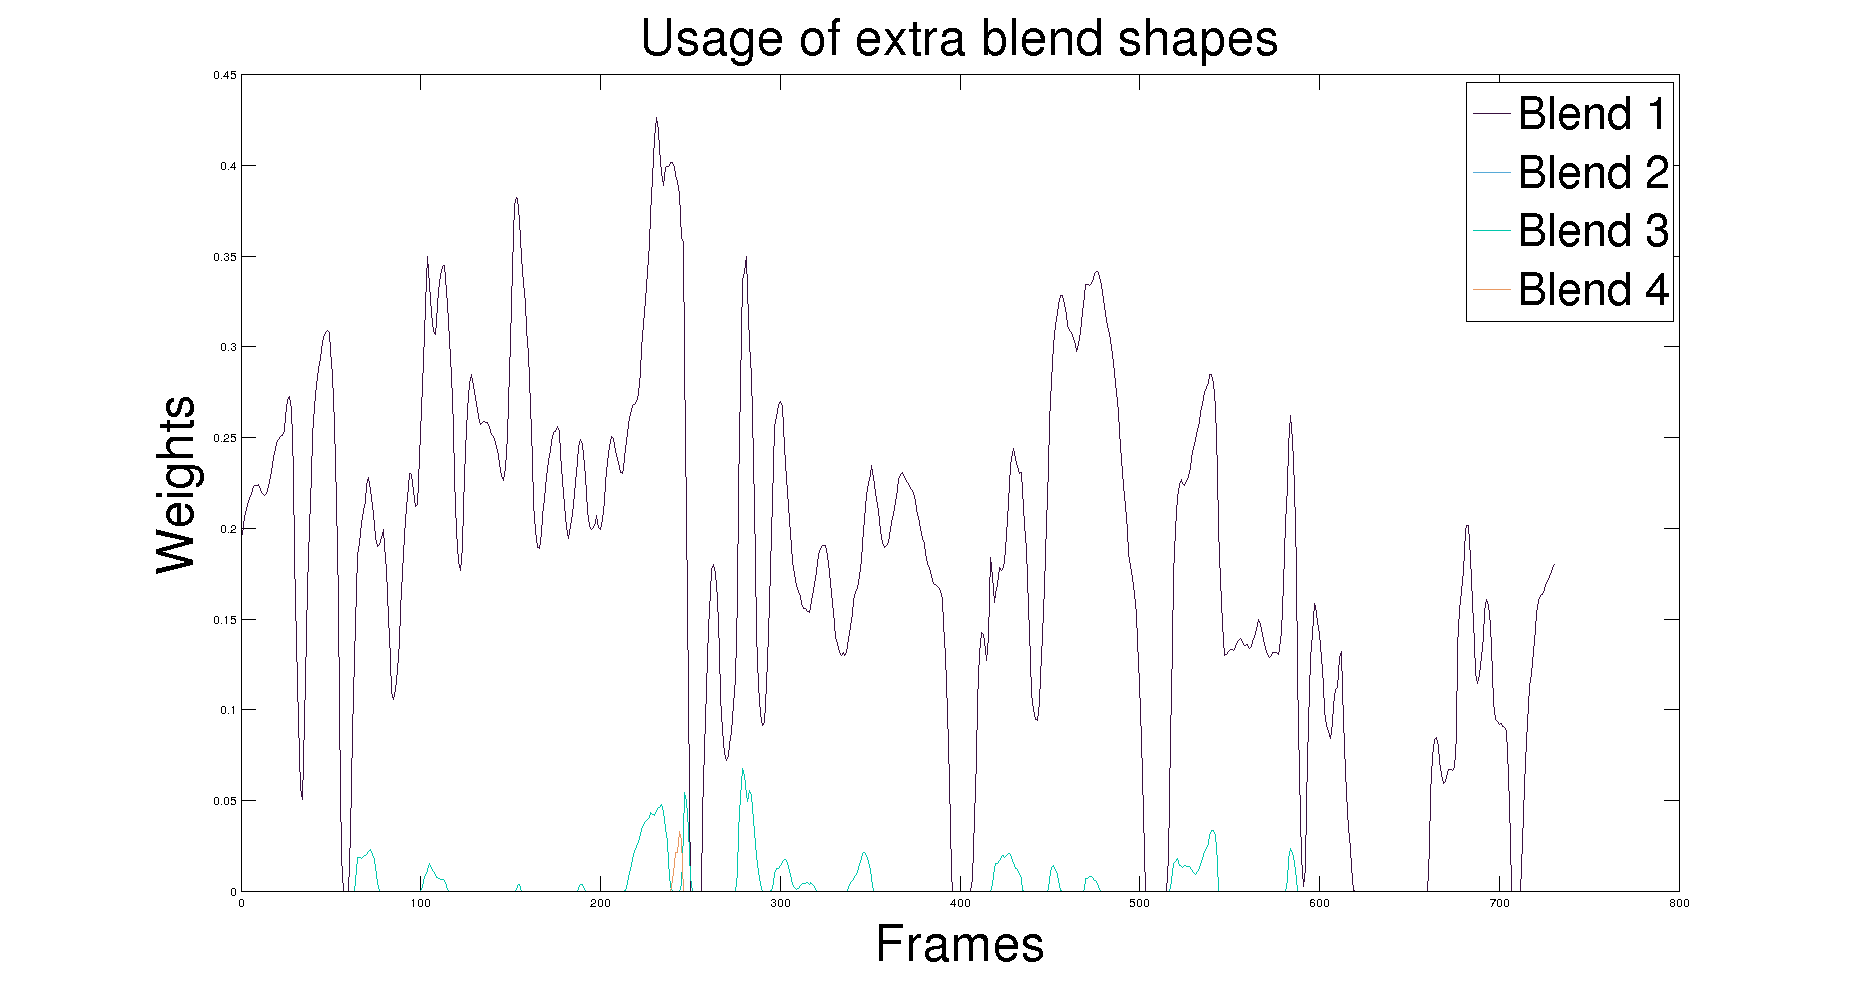
\includegraphics[trim = 10mm 0mm 10mm 0mm,clip,width=\textwidth]{img/weights/3D/Extrafaces/w2_72_usage.png}
        \end{subfigure}
        ~ %add desired spacing between images, e. g. ~, \quad, \qquad, \hfill etc.
          %(or a blank line to force the subfigure onto a new line)
        \begin{subfigure}[b]{0.47\textwidth}
                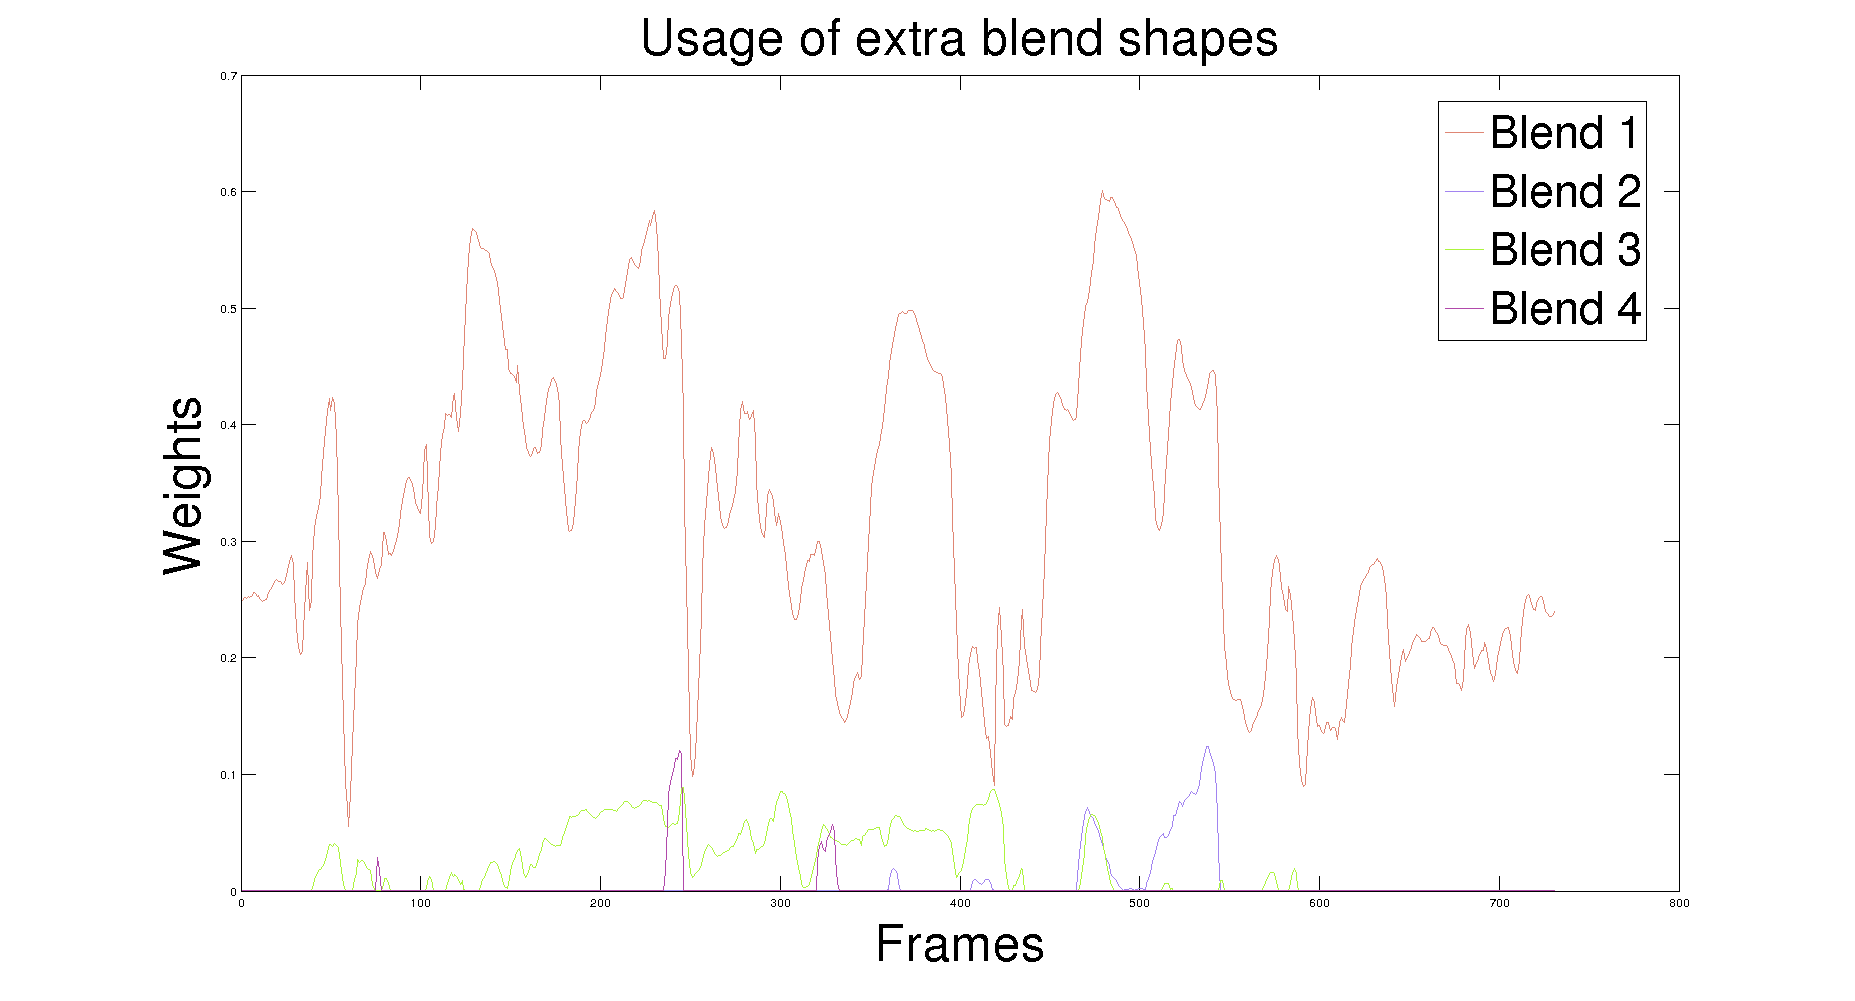
\includegraphics[trim = 10mm 0mm 10mm 0mm,clip,width=\textwidth]{img/weights/3D/Extrafaces/w3_72_usage.png}
        \end{subfigure}
        \caption{The weights associated with the extra blendshapes as a function of frames in the sequence. The left diagram corresponds to the constrained non-negative least-squares solver while the right one gives he results for the linear least-squares solver.}\label{fig:usage}
\end{figure}
Fig.~\ref{fig:usage} shows the activation of the extra blendshapes throughout the motion sequence. Both of the optimisation methods favour the first additional blendshape that corresponds to the smile in Fig.~\ref{fig:extrafaces} while the other shapes are only used with low weights. Despite the extension to the set of shapes, the reconstruction error decreased by less then $0.01$ centimetres for both methods. This is explained by the fact that the extra blenshapes are closely related to the original ones, as they are in fact a linear combination of the original blendshapes. A more systematic approach needs to be used to produce more diverse shapes. For example, an additional optimisation step may be included that randomly alters the existing blendshapes, and uses a small subset of the altered shapes to find the extension of the blendshape set that minimises the reconstruction error. In particular, we choose a set of new shapes that are constructed by adding a small random quantity to the average of the existing set. Then these shapes are included in the optimisation algorithm. The new shapes are stored if they reduce the reconstruction error, and new blendshapes are suggested until the error decreases below a chosen threshold. Using this iterative procedure, we are able to reduce the reconstruction error by about $10 \%$; however, this approach is very computationally intensive, and the new shapes cannot be easily included in the existing model. 

\subsubsection{Estimation of Weights in Actor's Domain}

At this stage our best results still lack expressiveness and visual appeal. In the current pipeline, we first transform the motion sequence from the actor to Emily, and then solve for the blendshapes in the Emily domain. This approach relies on the transformation to produce valid motion in the Emily domain; however, the transformation is geometrical, and it does not guarantee to produce a realistic and natural-looking animation. Therefore, we test the opposite approach. We first find the thin plate spline transformation $\mathbf{T}$ from the actor's neutral expression to Emily's neutral expression. Then the inverse transformation $\mathbf{T^{-1}}$ is used to map the Emily blendshapes to the actor's domain. We thus have matching sets of sparse blendshapes in both domains, see Fig~\ref{fig:EtoR}. The weights are calculated at each frame using the original captured sequence and the newly designed blendshapes in the actor's domain; these weights are then applied directly in the Emily domain. 

\begin{figure}[htbp!]
        \centering
        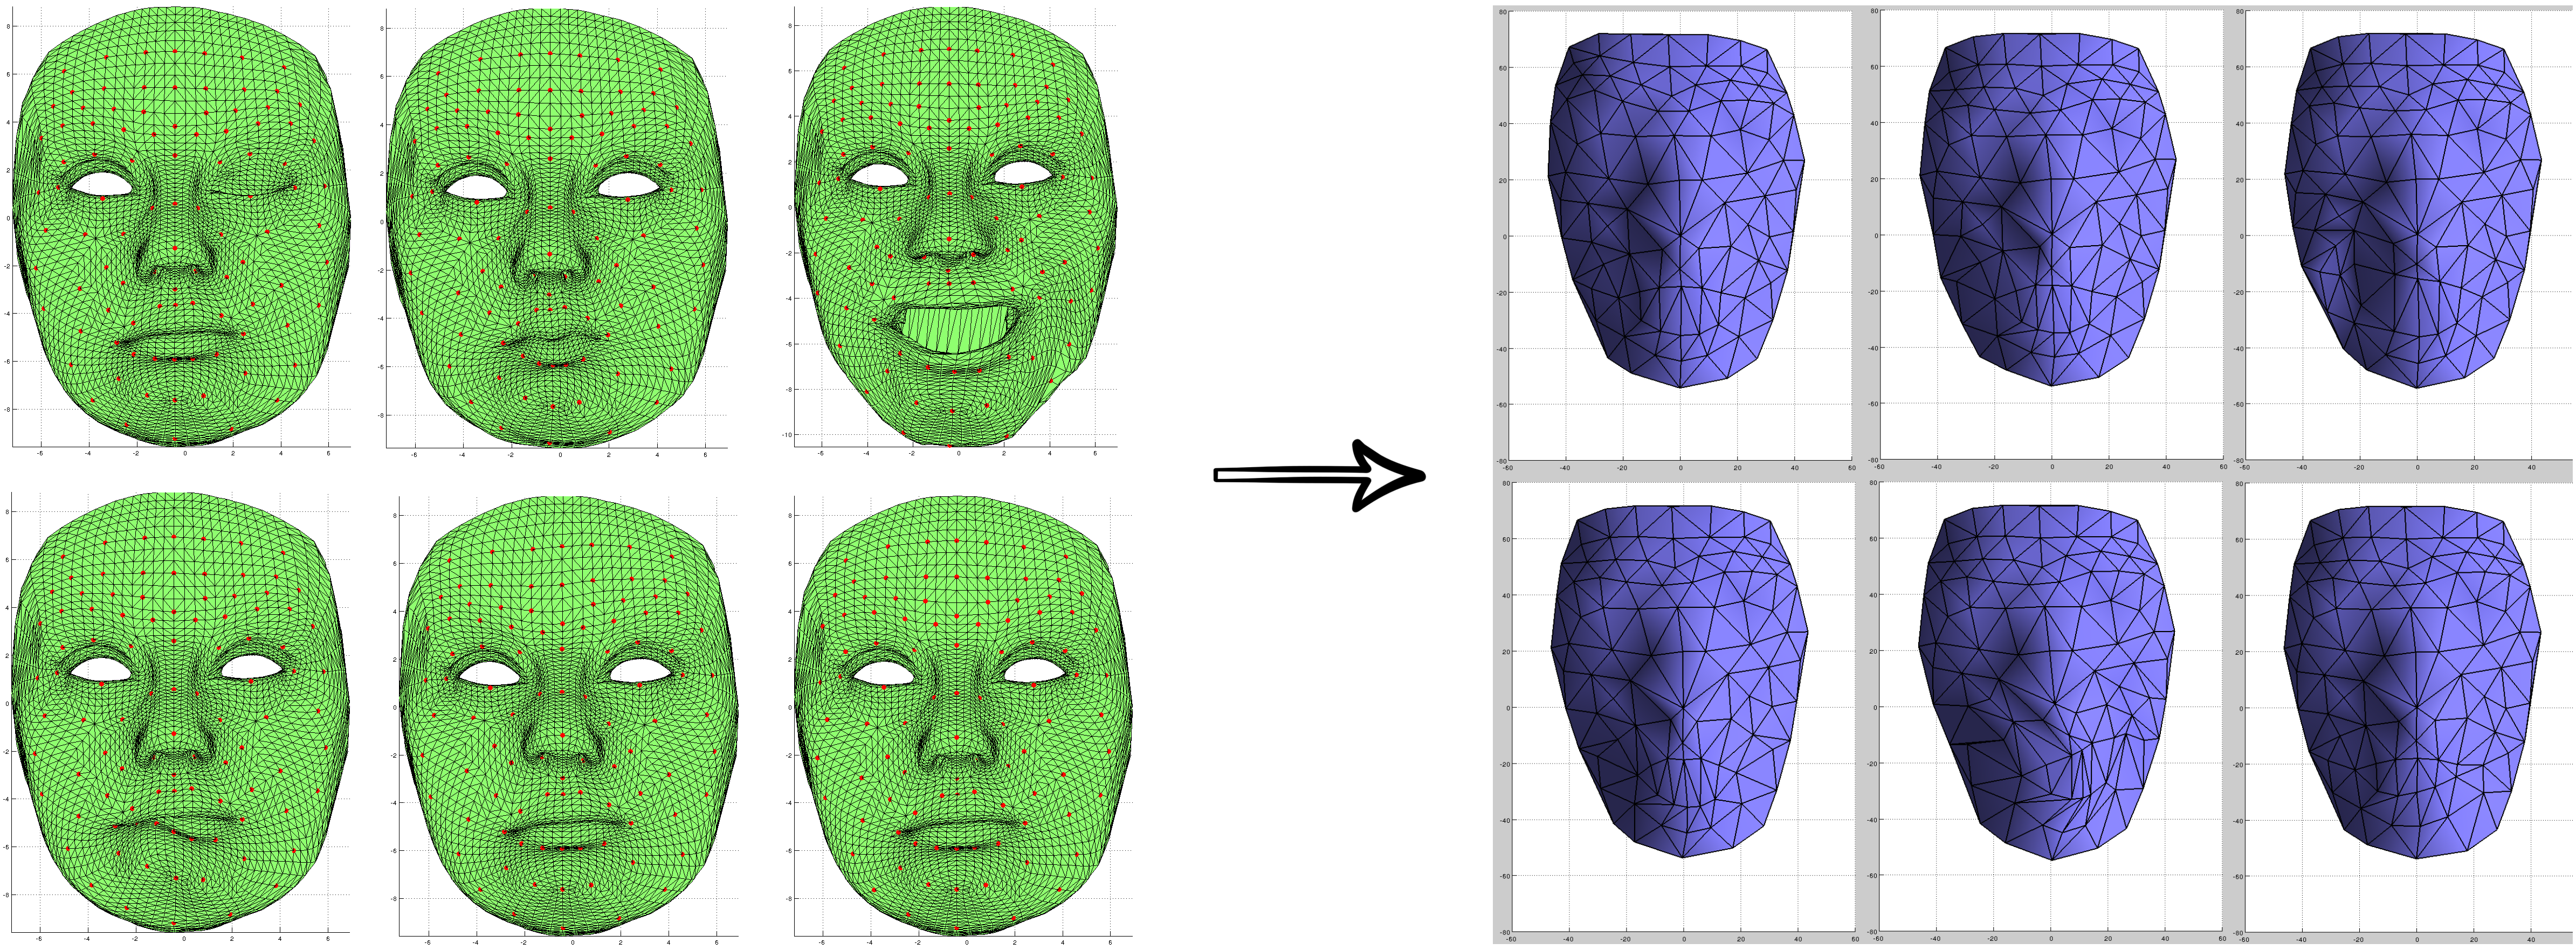
\includegraphics[width=0.8\textwidth]{img/EtoRblends}
        \caption{Use the inverse thin plate spline transform $\mathbf{T^{-1}}$ to produce a set of blendshapes in the actor's domain. The left images are the sparse Emily blendshapes (red dots) while the right images are the sparse actor's blendshapes (vertices of the mesh)}\label{fig:EtoR}
\end{figure}

Fig.~\ref{fig:resultcomp} compares the results produced using the two antipode approaches. The new approach is able to better mimic the motion of the actor, and it improves the appearance of the digital model, i.e. the new animation appears more natural and realistic. Note that the original method tries to reproduce the actor's performance using the transformed geometrical data while the new method relies more on the semantics associated with the blendshapes. In particular, we do not expect the actor and Emily expressions to match identically, for example one of them might be able to raise the eye-brows higher than the other. The new approach is better at respecting and enhancing the different features of the two faces. The mean reconstruction error is smaller than $0.01$ centimeters which is an improvement over the previous methods. We test our new approach using another motion capture sequence; in the new sequence the actor pulls the expressions listed in the Facial Action Coding System~\cite{FACS}. This sequence is more challenging as the expressions are diverse and intricate as opposed to the rather monotonous motion in the talking sequence.
\begin{figure}[htbp!]
        \centering
        \begin{subfigure}[b]{0.6\textwidth}
                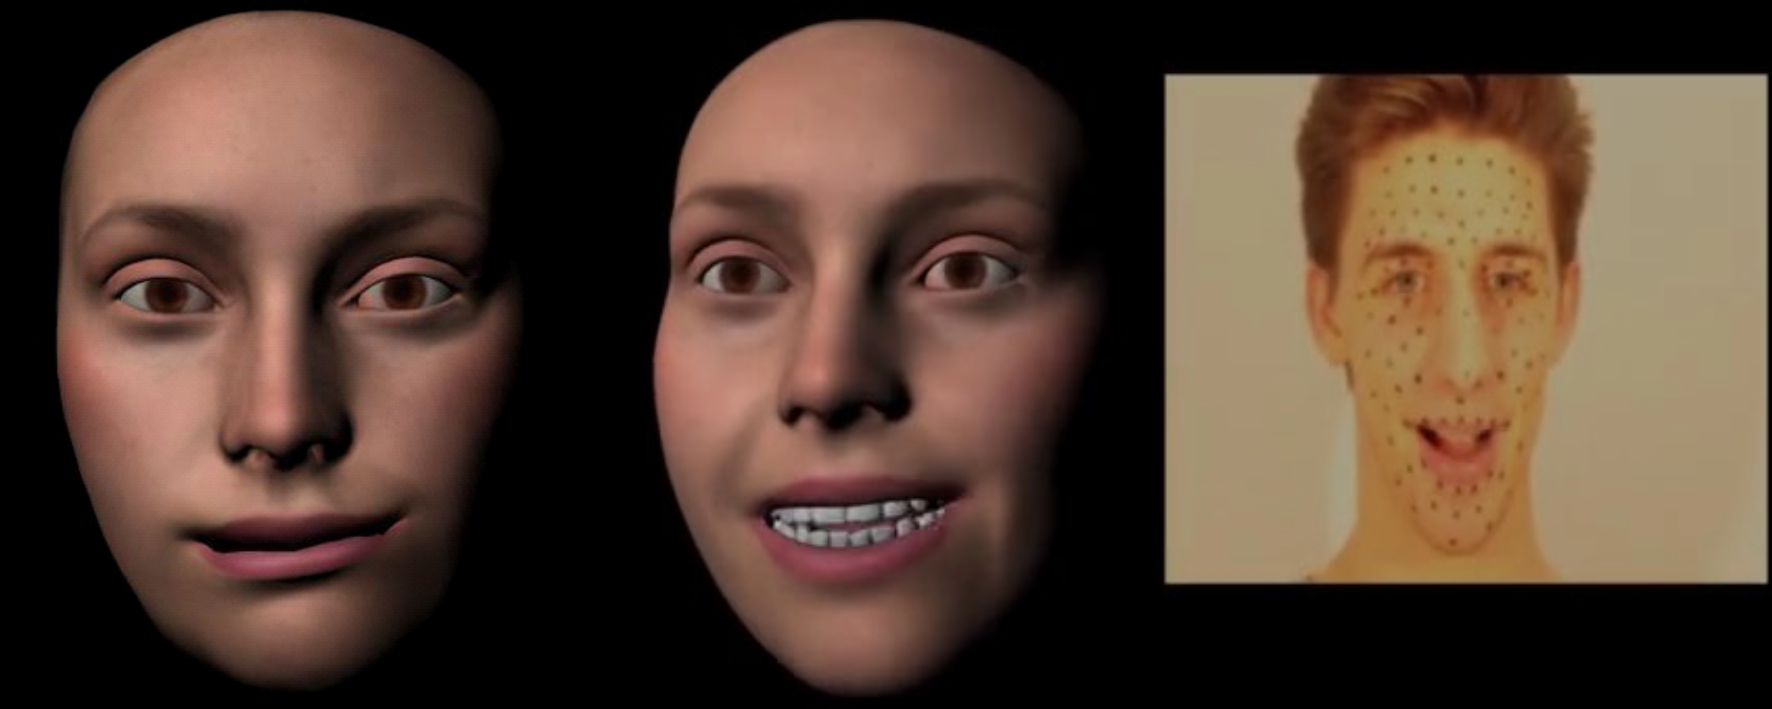
\includegraphics[width=\textwidth]{img/comp4s.png}
        \end{subfigure} \\
        \begin{subfigure}[b]{0.6\textwidth}
                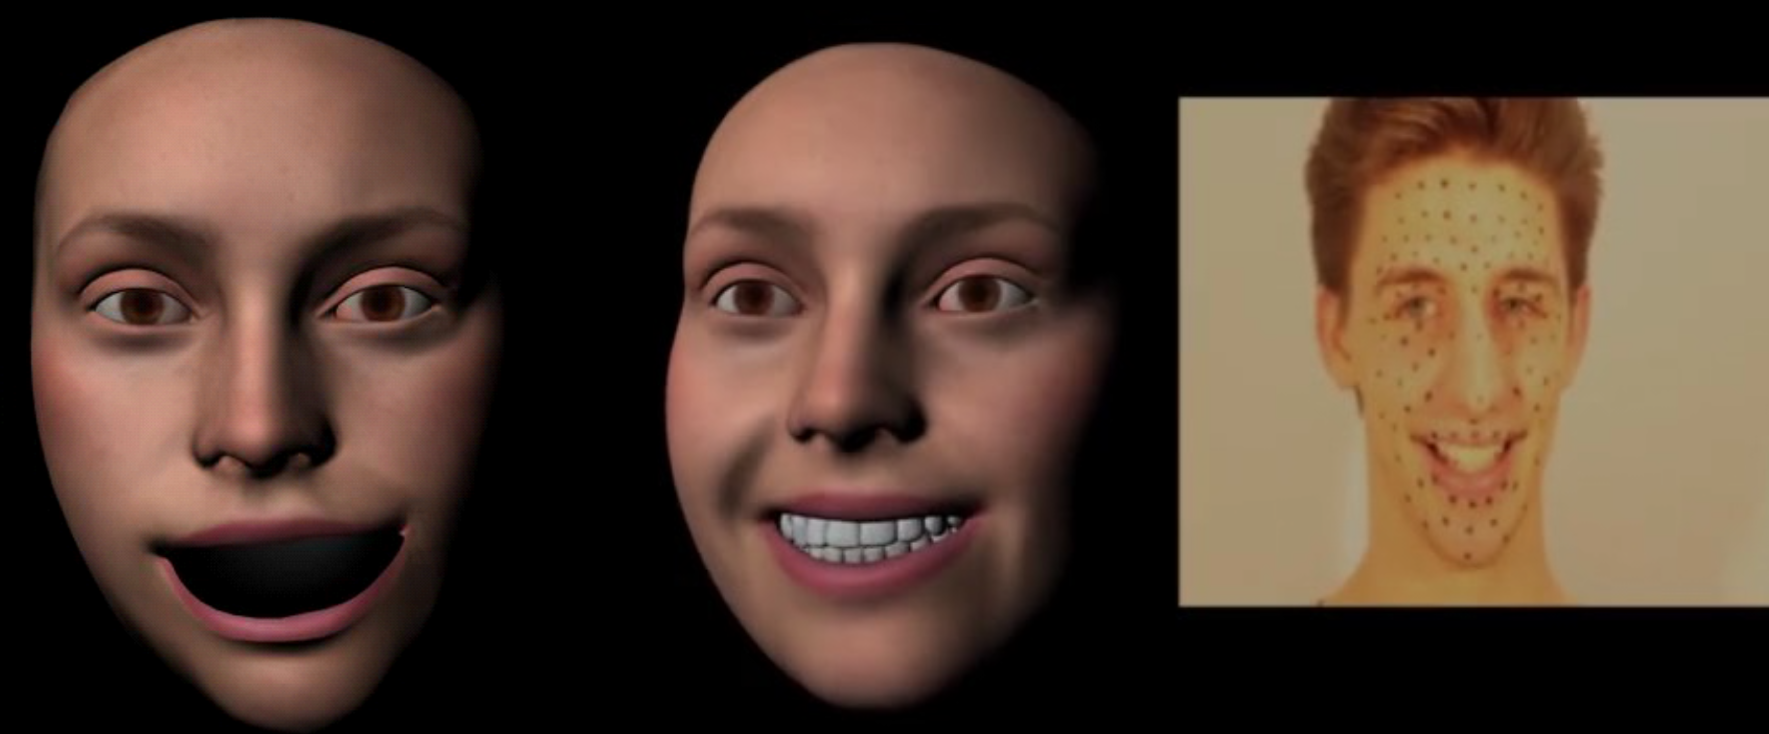
\includegraphics[width=\textwidth]{img/comp6s.png}
        \end{subfigure}
        \caption{The expressions on the left were produced using our original approach while the expressions in the middle use the weights that were calculated in the actor's domain. }\label{fig:resultcomp}
\end{figure}

We note that our final animation was not always able to capture the slight smiles that are noticeable in the recorded sequence. This may be explained by the poor match of neutral expressions. Specifically, all of the methods that we used rely on the transformation between the neutral faces. However, the actor's neutral expression is more positive (i.e. the corners of the lips are raised) than that of Emily, see Fig.~\ref{fig:neutrals}. This may be fixed by choosing a better matching neutral face from the actor's sequence, or by mimicking the actor's expression on Emily, and using that as her neutral. In our final results we use the second approach, and apply an additional small positive weight to the blendshapes that correspond to a smiling face, see Sec.~\ref{sec:implementation_details}.
\begin{figure}
        \centering
        \begin{subfigure}[b]{0.3\textwidth}
                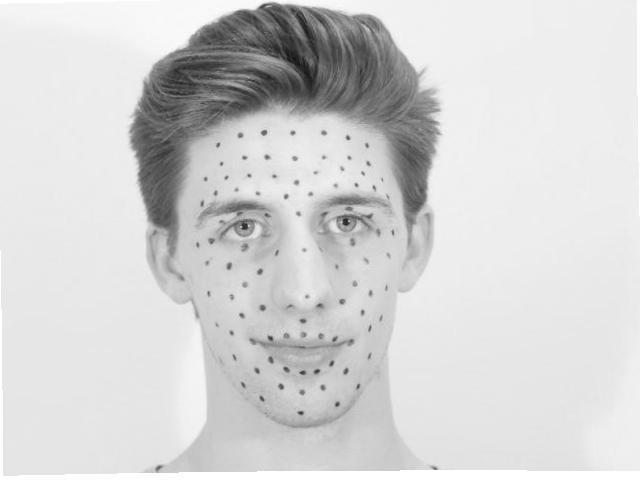
\includegraphics[width=\textwidth]{img/Richard2neutral}
        \end{subfigure}
        \begin{subfigure}[b]{0.4\textwidth}
                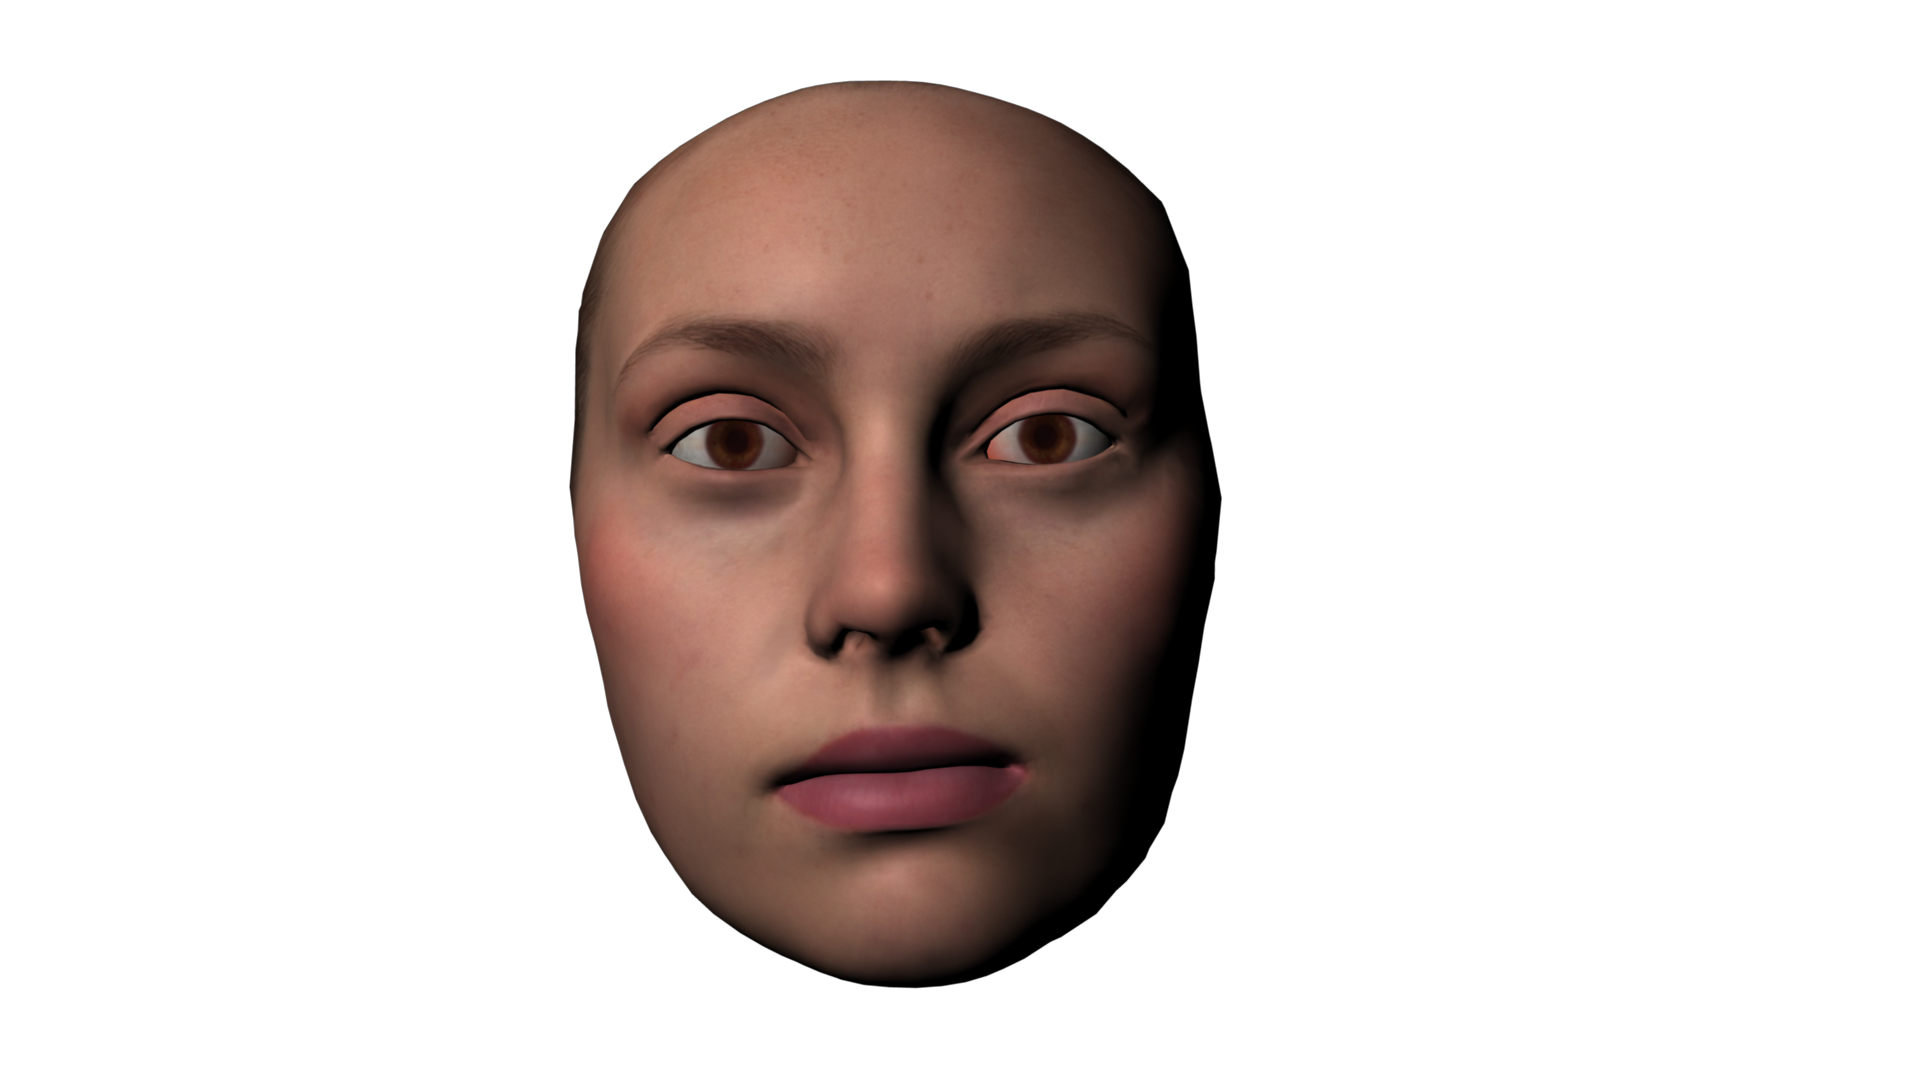
\includegraphics[width=\textwidth]{img/emily_neutral}
        \end{subfigure}
        \caption{The comparison of neutral expressions.}\label{fig:neutrals}
\end{figure}

\section{Skin Rendering}
\label{sec:metho_skin_rendering}

Our objective in skin rendering is to generate a face that would be indistinguishable from a real one.
In our case, we have have taken a 3D scan of a subject and our aim is to improve the realism when rendering it.
For this task we will mainly look at the techniques presented by Hertzmann et al~\cite{Hertzmann2001} and Graham et al~\cite{Graham2013}.

\begin{algorithm}[htbp!] 
	\caption{Image Analogies}
	\label{alg:image_analogies}
	\KwData{$A$ unfiltered example, $A'$ filtered example, $B$ unfiltered source, $L$ number of levels, $k$ coherence parameter, $t$ neighbourhood size.}
	\KwResult{$B'$ filtered source image.}
	
	Compute Gaussian pyramids for $A$, $A'$ and $B$\;
	Compute features for $A$, $A'$ and $B$\;
	Build k-d tree for $\left\lbrace A, A' \right\rbrace$\;

	\For{$l$ = 0 to $L$}{
		\For{each pixel $q \in B'_l$}{
			$p_{app} =$ ANN search of $q$ neighbourhood from $\left\lbrace B, B' \right\rbrace$\;
			$r^* = \mbox{arg}\min\limits_{r \in N(q)} \left \| F_l(s(r) + q - r) - F_l(q) \right \|^2$\;
			$p_{coh} = s(r^*) + (q - r^*)$\;
			$d_{app} = \left \| F_l(p_{app}) - F_l(q) \right \|^2$\;
			$d_{coh} = \left \| F_l(p_{coh}) - F_l(q) \right \|^2$\;
			\eIf{$d_{coh} < d_{app}(1 + k2^{l-L})$}{
				$p = p_{coh}$
			}{
				$p = p_{app}$
			}
			$B'_l(q) = A'_l(p)$\;
			$s_l(q) = p$\;
		 }
	}
	\KwRet{$B'_L$}
\end{algorithm}

Before we begin, lets explain the Image Analogies framework~\cite{Hertzmann2001} in more detail.
Given three images $A$, $A'$ and $B$, where $A$ is an unfiltered example, $A'$ is a filtered example, and $B$ is an input image, the algorithm will generate an output image $B'$ such that $B'$ relates in the same way to $B$, as $A'$ does to $A$.
A k-d tree for an Approximate Nearest-Neighbour Search (ANN) is built using a feature vector from a neighbour pixel $p$ in $A$ and $A'$.
The closest match for a neighbourhood in pixel $q$ in $B$ and $B'$ is located in the tree.
A detailed description of the algorithm in pseudo code is shown in Algorithm~\ref{alg:image_analogies}, where $F$ is computed a weighted distance over the feature vectors using a Gaussian kernel and $s$ is a data structure such that $s(q) = p$.
Based on Ashikhmin's work, a match that is coherent to what has been already synthesized is computed.
These two candidates are weighted and the best one is chosen.
The whole process is carried in a multiresolution pyramid, as shown in Figure~\ref{fig:ia_diagram}, where $l$ indicates the current level, in essence this means that the neighbourhoods also include the previous level in the search.
We found three Image Analogies implementations available \cite{ImAnSingleThreadWeb, ImAnCudaWeb, ImAnHertzmannWeb}.
The first one is a simple single threaded implementation, the second one was done with CUDA, however the author's single threaded code produced overall better results.

\begin{figure}[htbp!]
\begin{minipage}[b]{.55\textwidth}
\centering
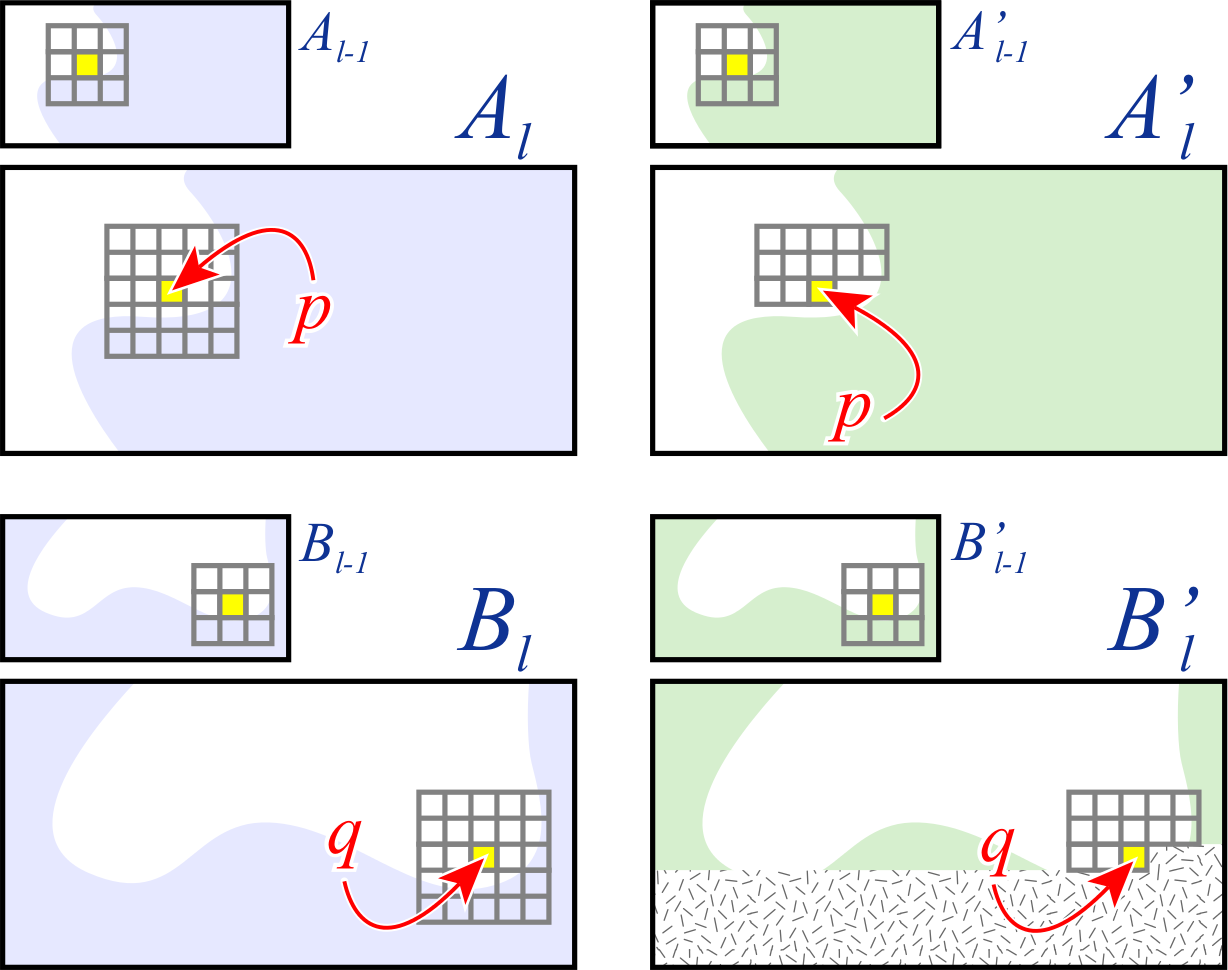
\includegraphics[width=\textwidth]{img/ia_diagram}
	\caption{ Neighbourhood matching for the Image Analogies framework, image taken from~\cite{Ashikhmin2001}.}
	\label{fig:ia_diagram}
\end{minipage}
\hfill
\begin{minipage}[b]{.4\textwidth}
\centering
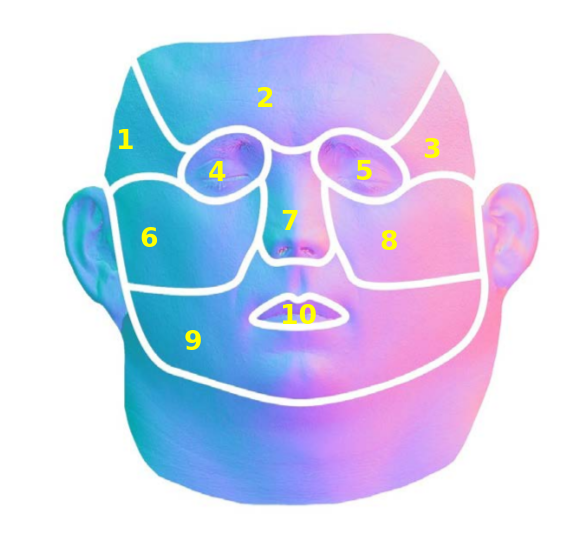
\includegraphics[width=\textwidth]{img/texture_synthesis_parts}
	\caption{ Texture segmentation in common coloured areas, image taken from~\cite{Graham2013}.}
	\label{fig:texture_synthesis_parts}	
\end{minipage}
\end{figure}

As a first step, we tried to reproduce the results for bump mapping quality increase by Graham et al~\cite{Graham2013}, results are shown in Figure~\ref{fig:bump_maps}.
The authors add an extra parameter $\alpha \in \left\lbrace 0, \ldots, 1 \right\rbrace$ to control Hertzmann's image synthesis process.
To be more precise, a match between $A$ and $\left\lbrace B,B' \right\rbrace$ will be weighted by $1 - \alpha$, and a match between $A'$ and $\left\lbrace B,B' \right\rbrace$ will be weighted by $\alpha$.
The logic behind this addition is to encourage more details of $A'$ to be included in $B'$.
The modifications required to include this addition begin by building two separated k-d trees for $A$ and $A'$, when choosing the best match both distances will be weighted as explained above and the smaller one will be chosen.
Also in the coherence match two searches will be done and weighted accordingly, and the final pixel will be chosen without further adjustments.

\begin{figure}[htbp!]
\centering
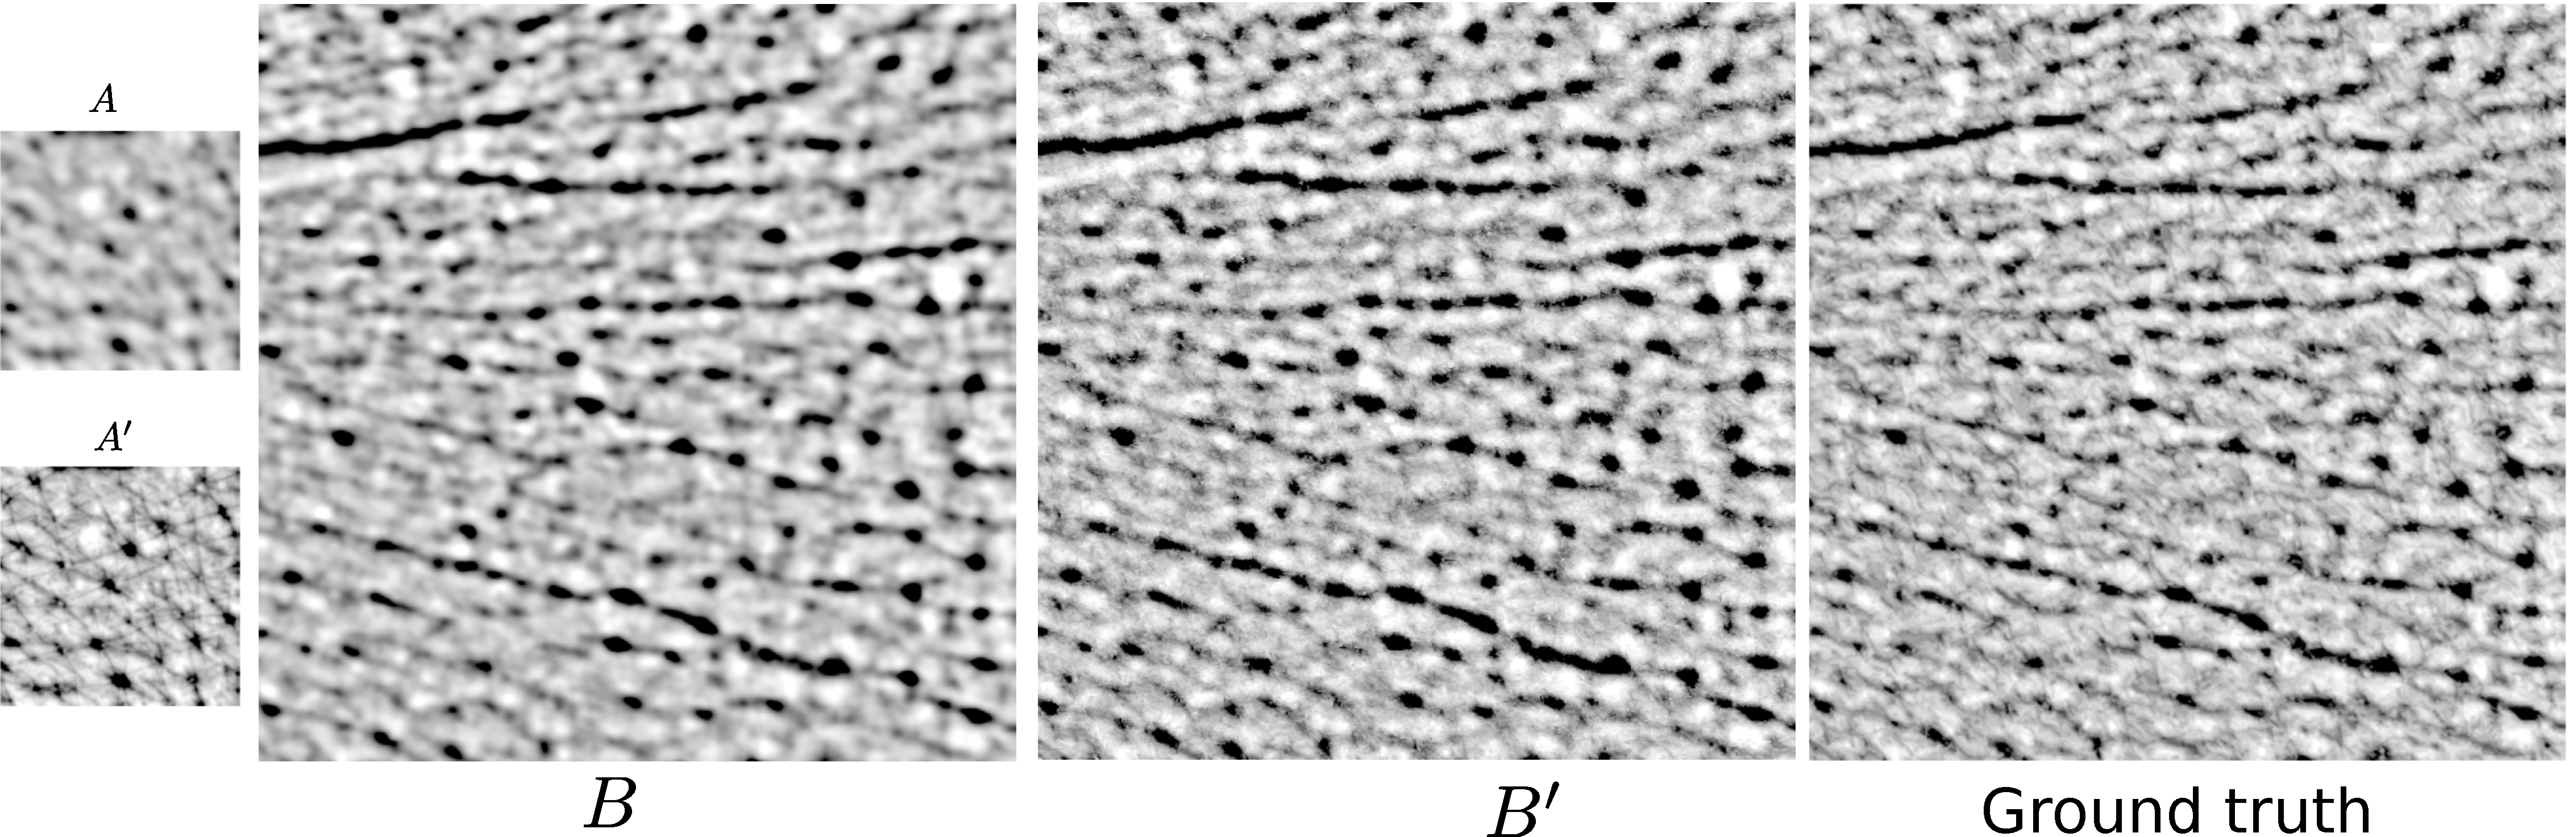
\includegraphics[width=\textwidth]{img/bump_maps}
	\caption{ Bum map deblurring, $A$, $A'$, $B$ and ground truth images images taken from~\cite{Graham2013}.}
	\label{fig:bump_maps}
\end{figure}

We also tried applying the Image Analogies filter to generate increased quality textures, which is in essence a deblurring filter.
The idea is to improve a low quality texture from a 3D scan using pictures of the texture taken at a closer range.
To achieve this we took a close up high quality sample $A'$, to generate $A$, the sample $A'$ was blurred using a Gaussian kernel until it look qualitative similar to the 3D scan texture $B$, with this three inputs we generated a picture $B'$ of higher quality.
Since faces have differentiated areas, this process was done separately for each relevant section in the face texture image, the generated patches are stitched together using linear interpolation.
The texture segmentation is shown in Figure~\ref{fig:texture_synthesis_parts} and results are shown in Figure~\ref{fig:texture_synthesis}.

\begin{figure}[htbp!]
\centering
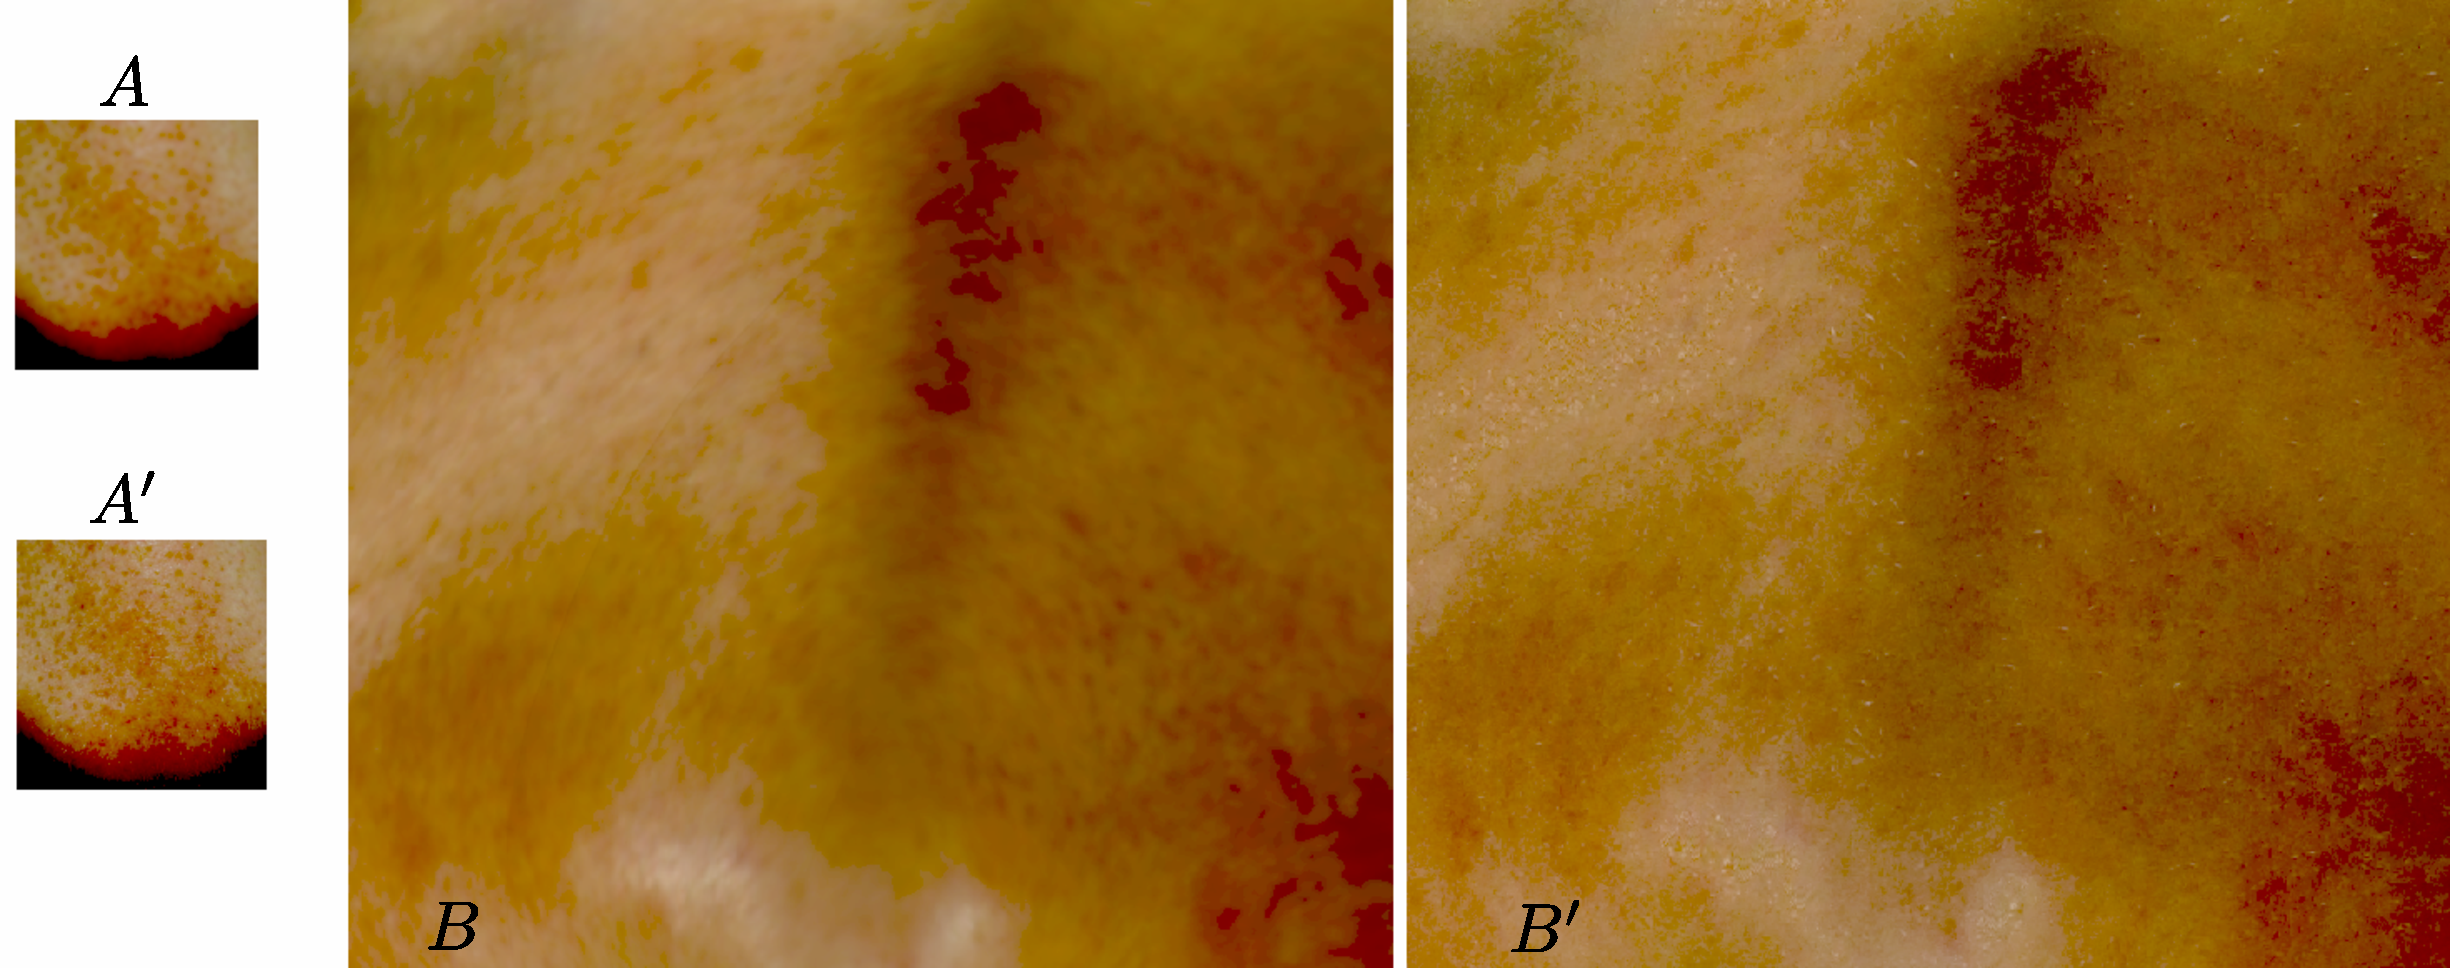
\includegraphics[width=\textwidth]{img/texture_synthesis}
	\caption{ Texture quality increase using image analogies, the texture is false-coloured to highlight the differences.}
	\label{fig:texture_synthesis}
\end{figure}

Another option for increasing the quality of the texture is to apply image super-resolution techniques, we used Jianchao et al~\cite{Jianchao2010} work for this purpose.
The idea is that by doubling the resolution of the original texture, yet avoiding blur by adding information from a dictionary of high resolution images, the final rendering quality of the face will increase.
Results for this approach are shown in Figure~\ref{fig:emily_super_resolution}.

\begin{figure}[htbp!]
\centering
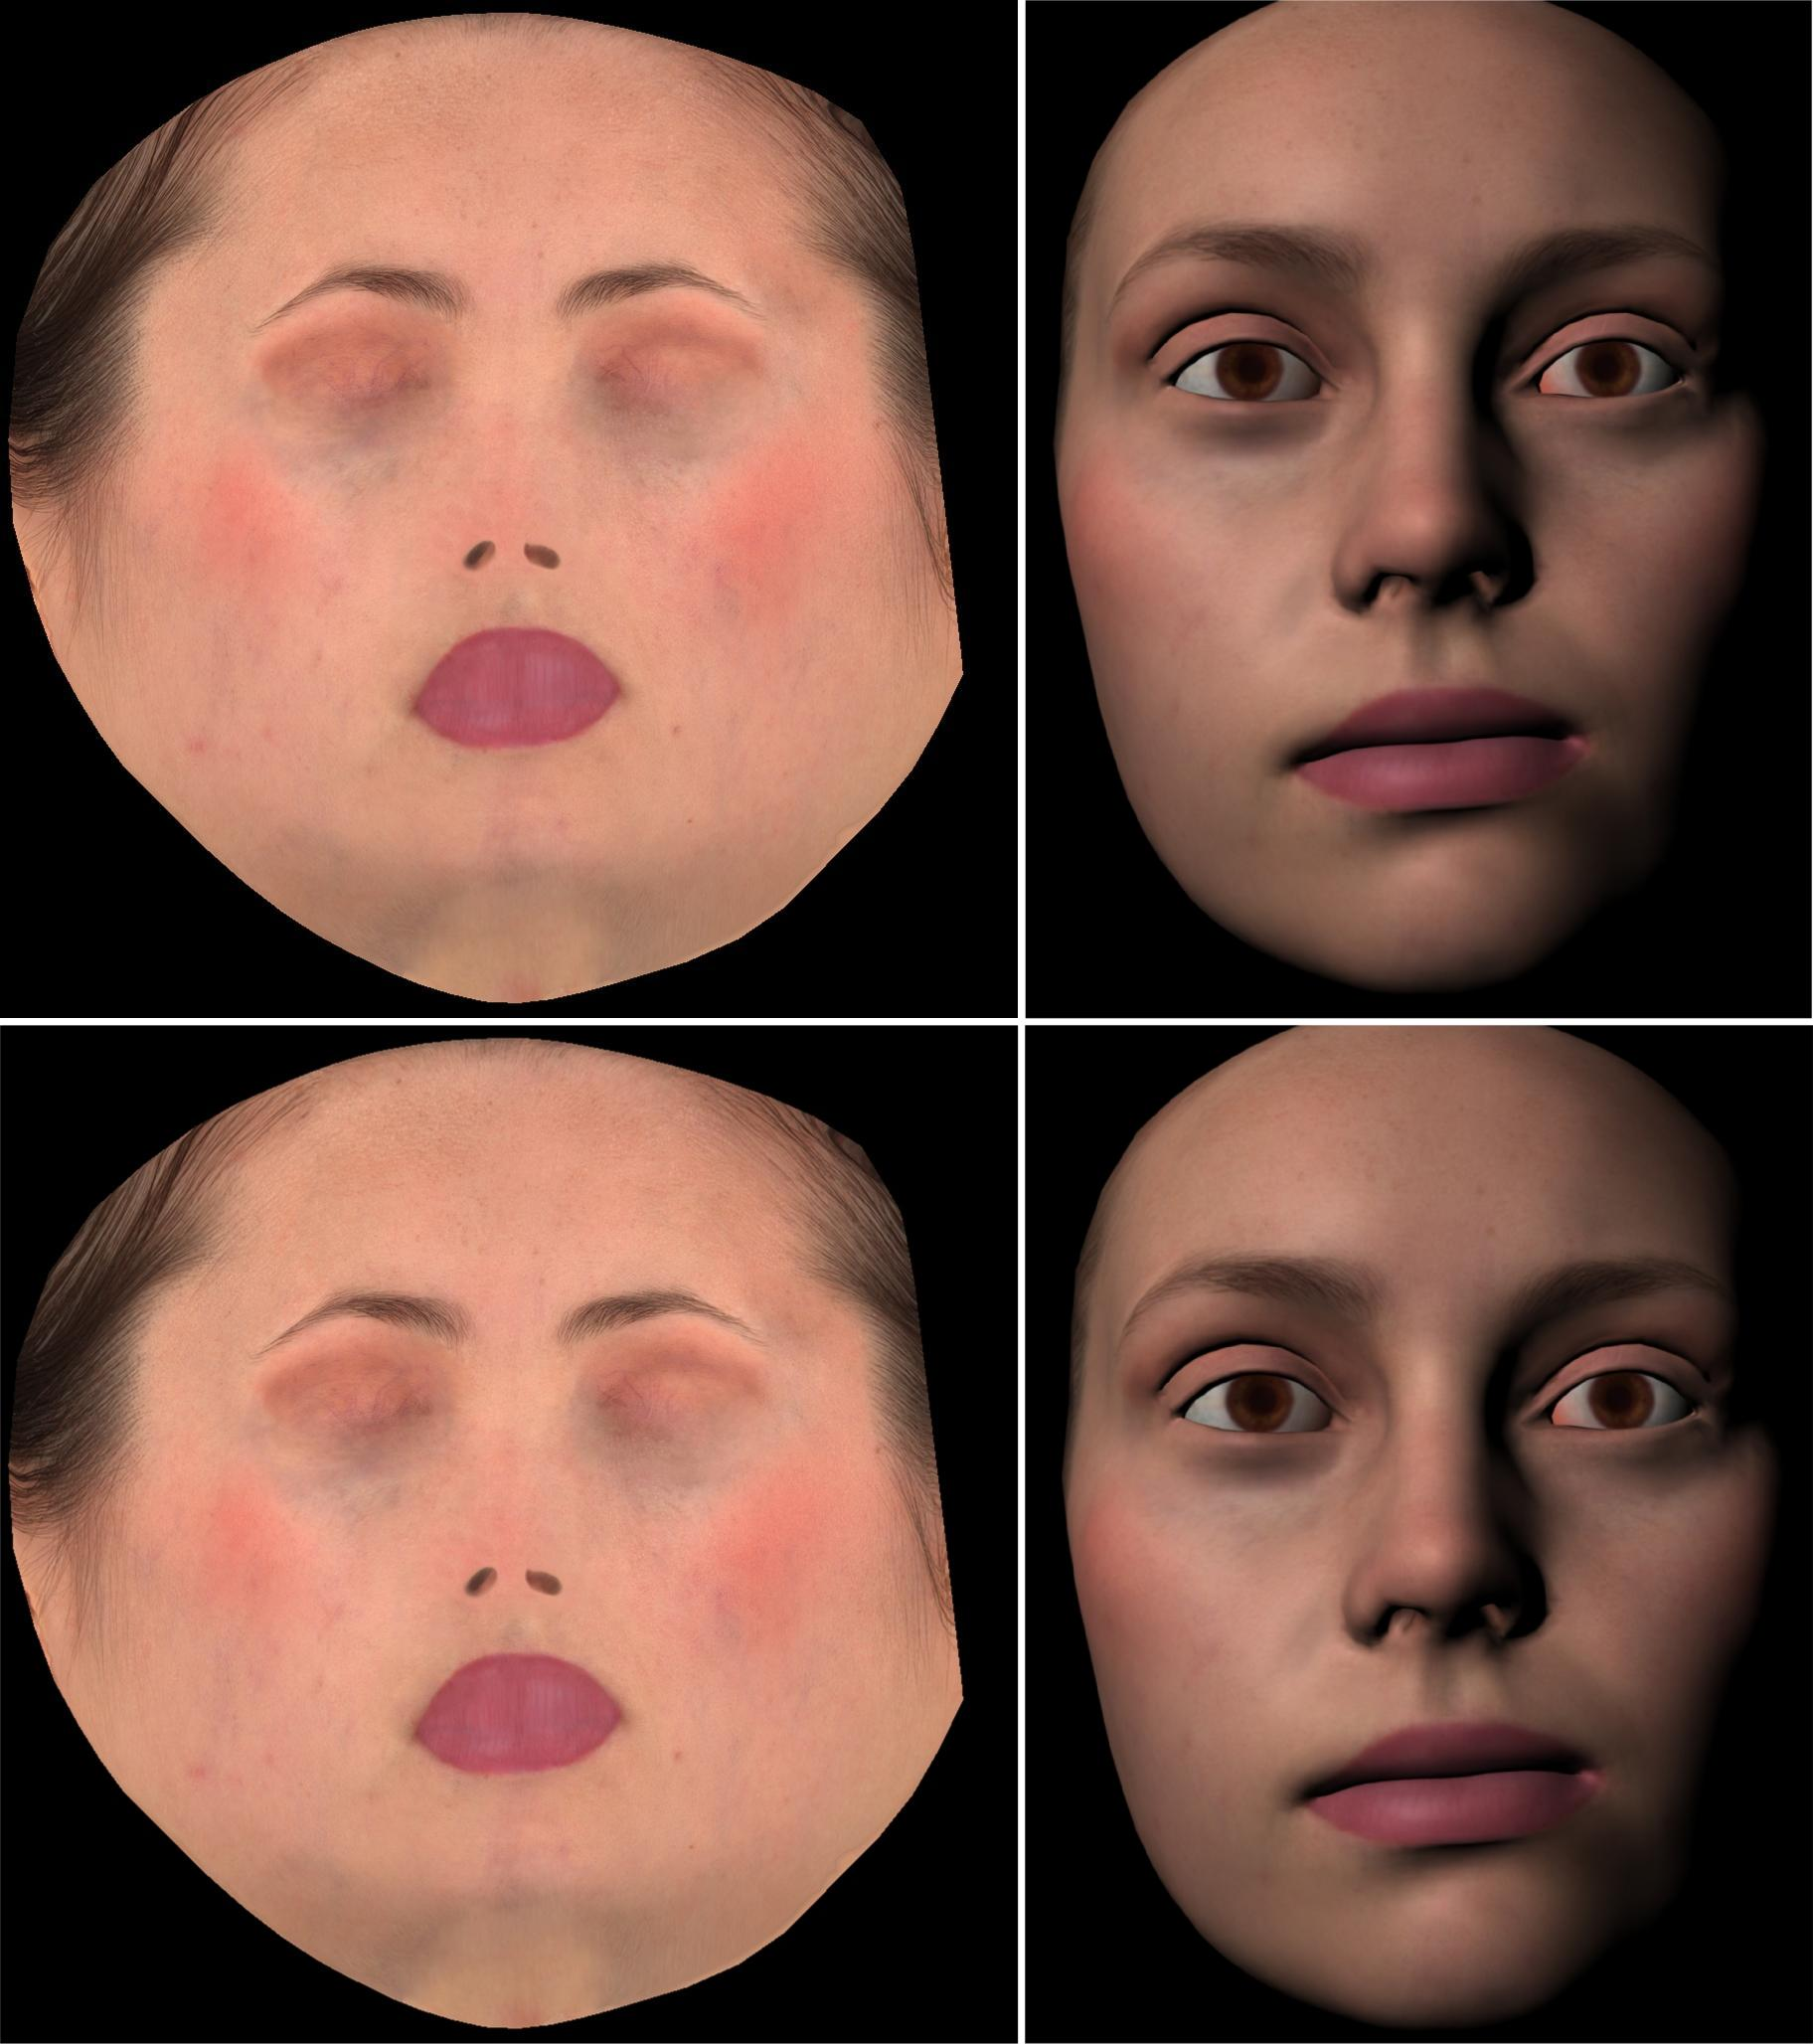
\includegraphics[width=\textwidth]{img/emily_super_resolution}
	\caption{ Super resolution example, left original texture, left-centre face rendered with original texture, right-centre super-resolution texture, right face rendered with super-resolution texture, original data from \cite{FaceWareWeb}.}
	\label{fig:emily_super_resolution}
\end{figure}

\begin{figure}
        \centering
        \begin{subfigure}[b]{0.48\textwidth}
                \includegraphics[width=\textwidth]{img/emily_close_original}
        \end{subfigure}
        \begin{subfigure}[b]{0.48\textwidth}
                \includegraphics[width=\textwidth]{img/emily_close_sr}
        \end{subfigure}
        \caption{Close up of texture super-resolution for Emily, (left) original texture, (right) synthesized texture with higher resolution.}
\end{figure}

Generating normals maps using Image Analogies is another interesting area, as it could provide an alternative to the costly standard capture methods.
For this we tried to generate a normal maps from albedo images and from bump maps generated from the previous 3D scan texture, results are shown in Figure~\ref{fig:normal_synthesis}. 
To create the bump maps, the textures were transformed to gray scale and a histogram equalization was applied.
In order to improve the quality of the bump maps, we also applied the Image Analogies filter to them using a known good bump map as a filtered example, results are shown in Figure~\ref{fig:bump_map_quality_increase}.

\begin{figure}[htbp!]
\centering
\includegraphics[width=\textwidth]{img/normal_generation}
	\caption{ Normal synthesis from albedo image.}
	\label{fig:normal_synthesis}
\end{figure}

\begin{figure}[htbp!]
\centering
\includegraphics[width=\textwidth]{img/bump_map_quality_increase}
	\caption{ Improving the quality of a bump map from a gray scale texture.}
	\label{fig:bump_map_quality_increase}
\end{figure}

The advantages of using a bump mapping are shown in Figure~\ref{fig:bump_mapping_richard}.
In this example, a render with the original texture is shown in Figure~\ref{fig:richard_original}.
The original RGB texture was converted to a gray scale image and applied directly as a bump map texture,
results are shown in Figure~\ref{fig:richard_disp_impr}, note how the addition of high frequency imperfections adds extra realism to the image.

\begin{figure}
        \centering
        \begin{subfigure}[t]{0.48\textwidth}
                \includegraphics[width=\textwidth]{img/richard_original}
                \caption{Render with the original texture.}
                \label{fig:richard_original}
        \end{subfigure}
        \begin{subfigure}[t]{0.48\textwidth}
                \includegraphics[width=\textwidth]{img/richard_disp_impr}
                \caption{Render with the original texture and bump mapping.}
                \label{fig:richard_disp_impr}
        \end{subfigure}
        \caption{The advantages of using a bump map..}
        \label{fig:bump_mapping_richard}
\end{figure}